\section{Chapter introduction}

Considering its impacts on the energy budget at the surface, the effects of irrigation follow a marked diurnal cycle, with distinct nighttime and daytime effects and varying amplitude depending on insolation. 
%option:could reuse refs from Intro
Average monthly or seasonal studies (like the work presented in Chapter \ref{chap:monthly}) cannot allow a detailed analysis of these impacts, and higher-frequency simulation outputs must be used.

Using the same simulation setup as Chapter \ref{chap:monthly}, this chapter focuses on the month on July 2021, and on part of the Ebro Valley. This study area and period were selected to include the measurement sites and special observation period (SOP) of the LIAISE field campaign. This enables direct comparison to local observations of temperature, humidity, wind and turbulent fluxes on irrigated and rainfed sites, at the surface and in the boundary layer. Furthermore, mesoscale modelling experiments were conducted over this area and period, in particular one with the Meso-NH model at 2-kilometer resolution that accounts for irrigation \citep{lunel_irrigation_2024}. This simulation served as an intermediate between point-based observations and the regional climate model, bringing new perspective on the following questions:

\begin{itemize}
    \item How does the ICOLMDZOR-LAM perform over the LIAISE study area, relative to observations and mesoscale simulation?
    \item To what extent does simulated irrigation improve the performance of the LAM? What limits its ability to reproduce observations on irrigated and rainfed sites at the diurnal scale?
    \item Are the effects of simulated irrigation limited to surface variables or do they propagate to the vertical structure of the ABL? 
    \item Are the effects of simulated irrigation only visible over the irrigated areas or do they also affect neighbouring rainfed areas?
    \item Over such a heterogeneous terrain, how can representativity of the LAM be defined and to what extent is it achieved for surface variables and the ABL?
    \item How does the heterogeneity of surface conditions affect the ABL structure and can these heterogeneities be accounted for by ICOLMDZOR?
\end{itemize}

This chapter first presents the LIAISE field campaign with details on the measurements and mesoscale simulation used, and relevant results of this project.
Then, the ICOLMDZOR LAM simulations used for comparison over LIAISE sites are described, before presenting results on land-atmosphere coupling variables and the vertical structure of the ABL.

\clearpage

\section{The LIAISE field campaign}
I would like to start by acknowledging that this description of the Land Surface Interactions with the Atmosphere over the Iberian Semi-Arid Environment (LIAISE) project is largely based on the various articles which presented the campaign : \citet{boone_land_2019,boone_updates_2021,boone_land_2025}, as well as on the dedicated section in Tanguy Lunel's PhD thesis \citep{lunel_interactions_2024}.

%objectives
LIAISE is an international research campaign aimed at improving the understanding of land-atmosphere-hydrology interactions in a semi-arid region characterized by strong surface heterogeneity owing to contrasts between the natural landscape and irrigation-dependent agriculture, and the limitations of models to represent all aspects of the terrestrial water cycle.

\subsection{Study area and meteorological conditions}

%period
Although the campaign included a longer monitoring of surface variables, this work focuses on the special observation period (SOP) which occurred from 15 to 29 July 2021. This SOP has been selected since it is the period where contrasts between irrigated and natural surfaces are generally at or near their maximum. At this time, synoptic scale winds are typically light and from the west, and a  thermal low pressure area generally forms over the region with daily maximum temperatures between 30 and 40°C.
Within this SOP, Intensive Observation Periods (IOPs) were selected, aiming for relatively clear days characterized by a well-mixed  atmospheric boundary layer with weak synoptic scale forcing, so that surface-induced local to regional scale circulations were most likely to be present and detectable. 

%area
The study domain for LIAISE is located within the Ebro basin in northern Spain, which is bound to the north by the Pyrenees, to the south by the Iberian System, and to the East by the less elevated Catalan Pre-coastal Range (Fig. \ref{fig:liaise_area_both}a). More precisely, it is within the Segre river sub-basin, which presents a semi-arid hot, dry  Mediterranean climate, with a very sharp delineation between a vast, nearly continuous irrigated region and the generally drier rainfed zone to the east of the study domain. The canal d'Urgell is a major irrigation infrastructure in the Segre basin that enables gravitational flooding of the irrigated area and effectively separates the irrigated and rainfed zones.
More recently, the Segarra-Garrigues canal was been built to the east of the Urgell canal, with the objective of providing water for irrigation in the eastern part of the Segre sub-basin.

\begin{figure}[hbtp]
    \centering
    \begin{subfigure}{\textwidth}
        \centering
        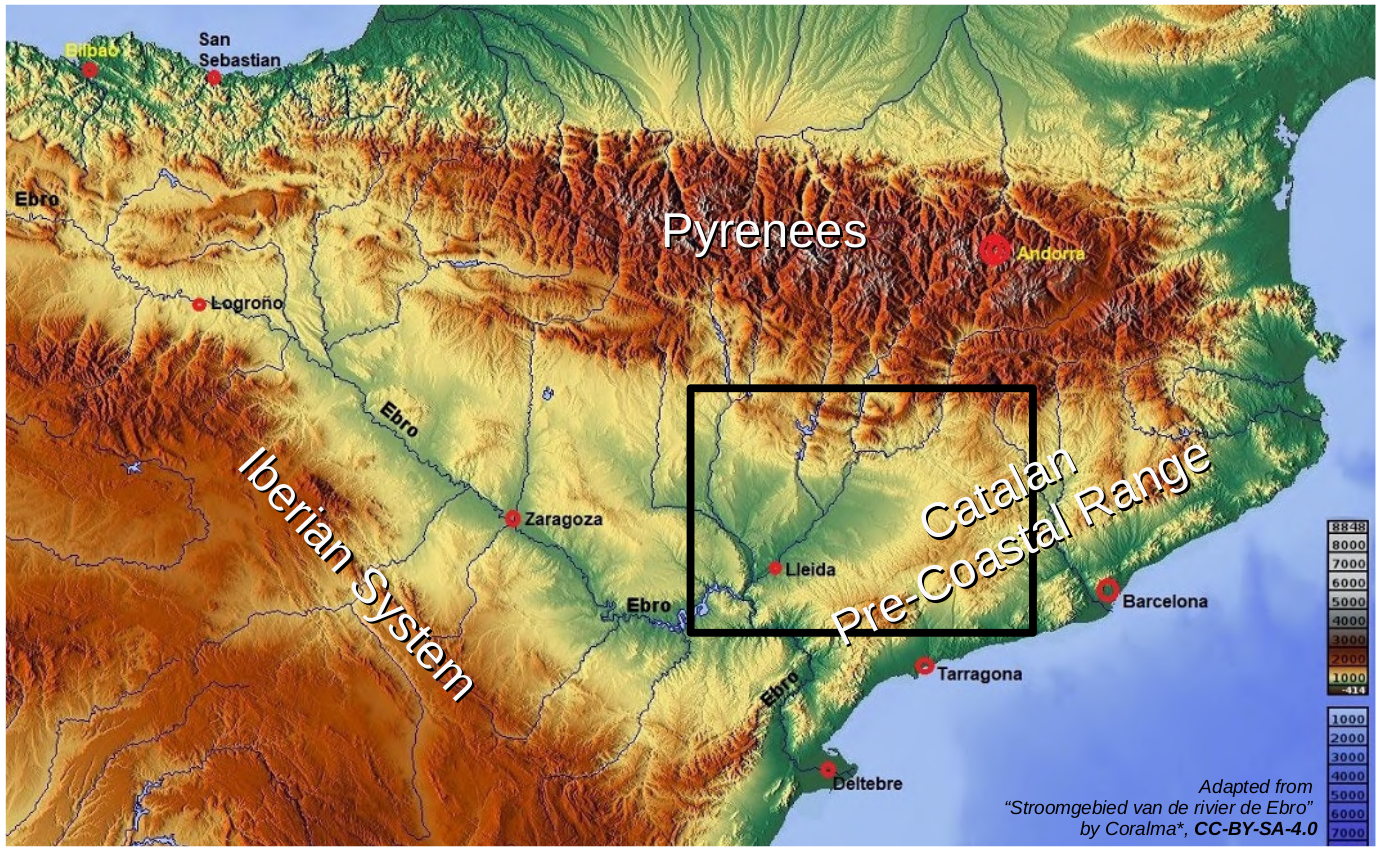
\includegraphics[width=0.8\linewidth]{images/chap6/liaise_area_ebro_lunel.png}
        \caption{Orography of the Ebro basin region. The three mountain ranges are indicated in white, and the black box corresponds to the zoom of (b)}
    \end{subfigure}
    %
    \begin{subfigure}{\textwidth}
        \centering
        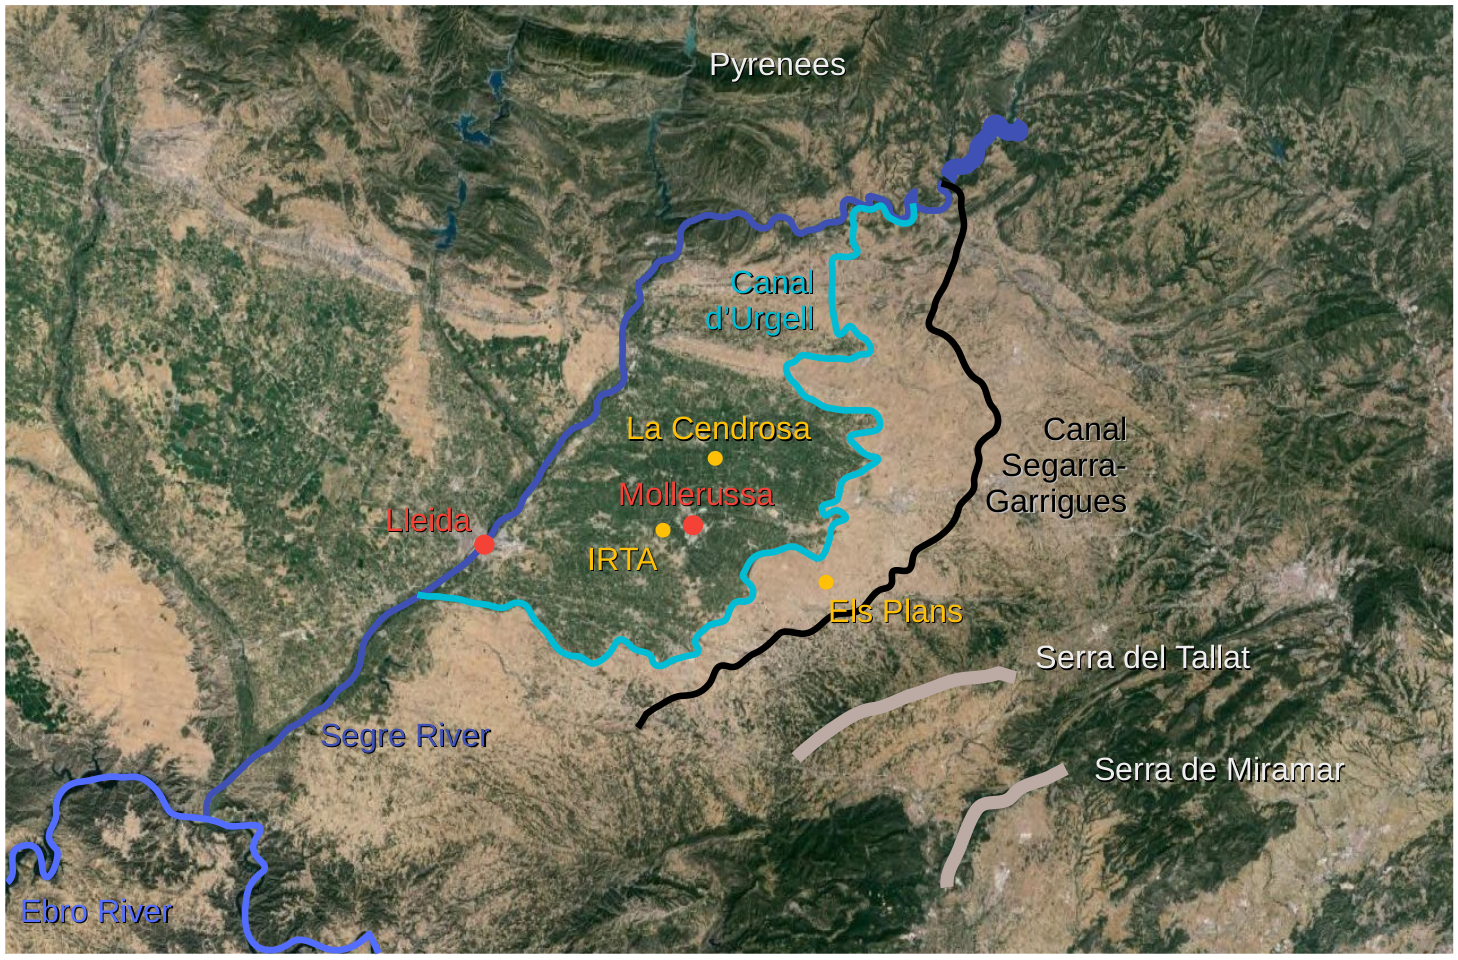
\includegraphics[width=0.7\linewidth]{images/chap6/liaise_area_zoom_lunel.png}
        \caption{Satellite visible image of the Segre river basin and its main topographic features taken by LandSat 7 in July 2021. The Segre and Ebro rivers are shown in dark blue, the Urgell canal in cyan and the recently built Segarra-Garrigues canal in black. The mountain ranges are in light brown. In red are the two main cities of the area and in yellow are the main instrumented sites of the LIAISE campaign.}
    \end{subfigure}
    \caption{Overview of the LIAISE study area. Both figures were taken from \citet{lunel_interactions_2024}.}
    \label{fig:liaise_area_both}
\end{figure}

%sites
Two supersites were defined at La Cendrosa, within the irrigated zone, and Els Plans, within the rainfed zone. Each was equipped with a 50-meter mast to measure temperature, humidity, wind speed and direction, radiative and turbulent fluxes (using eddy-covariance) at various heights.
Here are excerpts from the description of both sites given in \citet{lunel_interactions_2024}:
\begin{quote}
    ``La Cendrosa is one of the two sites along with Els Plans, which was equipped with numerous instruments to allow an in-depth study of its ecophysiological, soil and meteorological conditions. It is located well inside the heavily irrigated area [...], at an altitude of 240 m a.s.l., and on an almost flat area, with a slope of about 0.5\% towards the west.
    The alfalfa field where the instruments were installed is approximately 300 m x 200 m. Alfalfa is a perennial plant used to feed livestock and can be mown several times (including multiple growth cycles in a single summer). The alfalfa in the field was mown on 5 July 2021 and it regrew progressively over the rest of the month. [...] At the beginning of the two week period, the low LAI of the field affected the Bowen ratio measured above the field. It was observed that the Bowen ratio gradually decreased until it became constant around 21 July (not shown). La Cendrosa was flood irrigated twice in July, on the nights between 10 and 11 and between 23 and 24."
\end{quote}
\begin{quote}
    ``The site of Els Plans is a rainfed fallow land. It contains very little vegetation, and this vegetation was mainly dry during the SOP. It is located at the foothills of the Catalonian Pre-coastal Range, on a very gentle slope of about 1\% facing north-northwest, at an altitude of 334 m a.s.l. Els Plans is located about 3 km southeast of the irrigated-dry boundary."
\end{quote}

This work used 2-meter measurements of land-atmosphere coupling variables and 10-m wind (Section \ref{sec:sop}).
On IOP days, hourly radiosondes were launched, roughly from  sunrise through early evening, probing the ABL up to about 3 km. These measurements are used in Section \ref{sec:iop} to analyse the vertical structure of the atmosphere on 15 and 20 July.
Over the SOP, meteorological conditions were described as dry and hot, and only one precipitation event occurred, on 26 July. It was due to a thunderstorm which brought more than 25 mm to La Cendrosa but then propagated northeast and didn't affect the Els Plans site.
%option: wind regimes ? dominant, details on sea breeze...

\begin{figure}[hbtp]
    \centering
    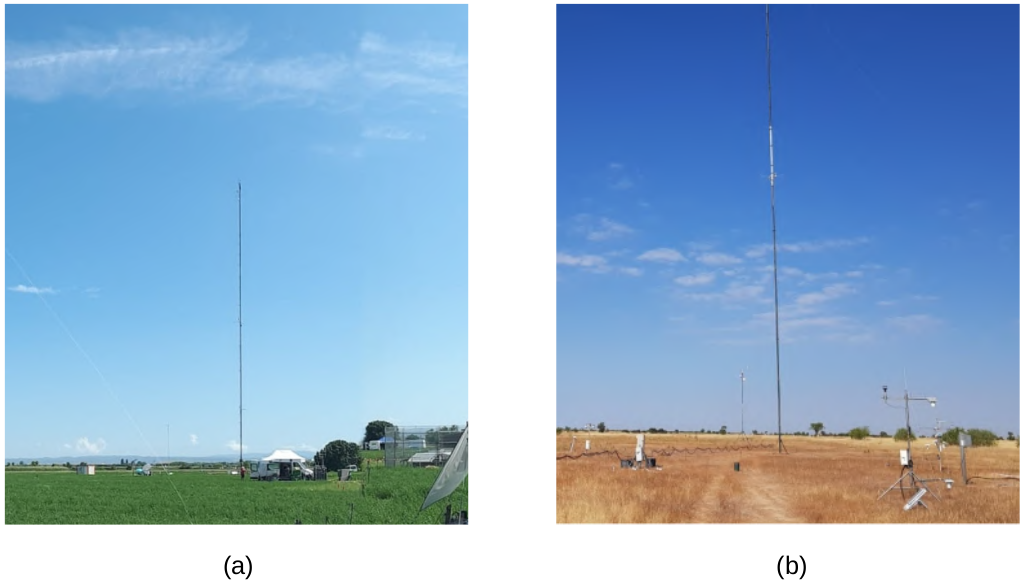
\includegraphics[width=\textwidth]{images/chap6/liaise_sites_picture.png}
    \caption{Instrumented sites of La Cendrosa (a) and Els Plans (b) in July 2021 \citep[taken from ][]{lunel_interactions_2024}.}
    \label{fig:liaise_sites_photos}
\end{figure}

%option: more details on choice of IOP days, synoptic conditions
%  This thermal situation has  a strong impact on surface winds. Formation of some shallow cumulus is possible, but moist convection, if present, is  generally confined to the surrounding mountain ranges. Owing to the proximity to the Mediterranean Sea to the east, sea  breeze (SB) formation is quite frequent, but its inland progression is slowed by the presence of the Catalan pre-coastal and  coastal ranges that separate the Ebro basin from the sea. The  intensity of the westerlies and strength of the heat low are also  contributing factors to the SB front propagation and intensity. Generally speaking, the SB front usually arrived sometime  between 16:00 and 19:00 local time over the study zone with  the dry zone sites impacted earliest. The SB passage was seen  in the observations as a low level wind shift (to winds with a  significant easterly component) over the entire region, while in  the east, horizontally-scanning lidar observations also revealed  a significant increase in low-level moisture with its arrival. The  sea breeze generally coincided with a collapsing ABL in the late  afternoon. Days with a predicted early arrival of the SB were  not designated as IOPs during the daily briefings. Finally, one  rain event did occur on July 26, which was associated with the  passage of a synoptic scale trough: local precipitation totals of  around 30 mm were recorded over the irrigated zone; however,  the convective cells propagated to the northeast and the dry zone received relatively little rainfall, thereby reinforcing the  wet-dry zone contrast during the subsequent days of the SOP.

\subsection{First results from observations and modelling}

The observations data from the LIAISE project has already been used in comparisons to mesoscale models to assess the relevance of simulating irrigation. 

The multi-model comparison presented in \citet{jimenez_land-surface_2025}, analysed simulations with Meso-NH  \citep{lac_overview_2018}, the Unified Model \citep{bush_second_2023,walters_met_2017} and WRF \citep{skamarock2021description} over the region. This study was initiated before the campaign took place and simulations were conducted without irrigation. It identified limitations of all models over the irrigated portions of the study area and concluded ``that it is important to take this process into account in order to capture land-atmosphere interactions properly".

Later, \citet{lunel_irrigation_2024} conducted simulations with and without irrigation, with the Meso-NH model at 400-meter resolution, nested into a larger Meso-NH simulation at 2-kilometer resolution. 
In these simulations, irrigation is represented in ISBA module of the SURFEX LSM \citep[Surface Externalisée,][]{masson_surfexv72_2013} by identifying irrigated areas in the land cover input map to associate them to a higher LAI, and maintain soil moisture at field capacity throughout the simulation.
On 20 and 22 July, it showed very significant improvement of simulated near-surface conditions at La Cendrosa when using irrigation, with a 4.7°C decrease in 2-meter temperature and a 50\% increase in 2-meter specific humidity during the day. The impacts of irrigation were not confined to surface variables but also influenced the structure of the ABL, achieving more stable profiles over La Cendrosa which matched the radiosoundings at 12UTC on both days. 
Tanguy Lunel kindly provided the outputs from the 2-kilometer simulation with irrigation, which were used as a gridded reference to complement the point-based observations of the campaign and allowed for the exploration of sub-grid heterogeneities in ICOLMDZOR, as presented in the following sections.

In a similar setup with the WRF model, \citet{udina_irrigation_2024} also found better model performance for near-surface air temperature, humidity, and wind speed and direction when the model included the irrigation parametrization. They noted lowering of the ABL around irrigated areas and a weakening of the existing sea breeze circulation, which is also described in \citet{lunel_marinada_2024}.
However, irrigation was not associated with a better representation of precipitation over the SOP (mainly the thunderstorm on 26 July) which was mostly driven by large-scale processes.

LIAISE data was also used to study the evolution of the ABL, \citet{brooke_irrigation_2023} highlighted the high impact of the contrasts induced by irrigation through the morning transition. 
\citet{mangan_evapotranspiration_2023} studied three scales of heterogeneity (10 km, 1 km, 100 m), to characterize their impact on surface energy partitioning and evapotranspiration, using the atmospheric mixed layer, slab model Chemistry Land-surface Atmosphere Soil Slab model \citep[\href{https://classmodel.github.io/}{CLASS},][]{arellano_atmospheric_2015}. They found surface-driven processes (radiation, surface layer) to be more important drivers of ET at the local scale ($\sim$100 m) than at the regional one  ($\sim$10 km), compared to boundary layer feedbacks. 
Combining this conceptual framework with additional LIAISE observation data, \citet{mangan_surface-boundary_2023} concluded that the observed ABL height was mostly determined by surface fluxes at the regional scale rather than local one, and that non-local boundary layer feedbacks also impacted local surface fluxes.

\hfill

All these results raised interest and questions on the ability of a regional climate model such as the ICOLMDZOR LAM to capture the impacts of irrigation on land-atmopshere coupling processes over the LIAISE study area, particularly considering the very limited representation of sub-grid heterogeneity in LMDZ and ORCHIDEE.

\clearpage

\section{Simulation experiments with ICOLMDZOR}

Several simulations are compared to analyse the diurnal cycle of land-atmosphere coupling variables in the Ebro Valley.
First, the two simulations studied in Section \ref{sec:article1} (\noirr and \irr) were analysed and compared to LIAISE observations using hourly outputs over the month of July 2021. However, irrigation volumes in the \irr simulation were quickly found to be overly constrained by water supply over the grid cell corresponding to the irrigated site of La Cendrosa. Sensitivity experiments were therefore conducted to increase irrigation, leading to the simulation referred to as \irrboost. This simulation was only run over the month of July, starting from the same state as \irr on 1 July 2021, and involved significant changes in both irrigation demand and water availability.

Regarding demand, the irrigated fraction was slightly increased to make sure that all of the soiltile dedicated to low vegetation and crops was considered as irrigated land. This soiltile represents 83.5\% of the grid cell, the rest being occupied by trees (12.4\%) and bare soil (4.1\%) which cannot be irrigated in ORCHIDEE. This fraction was also reduced to 0\% on the Els Plans site to make sure there would be no irrigation demand computed in this grid cell. This enables a better comparison to observations on this site but not the analysis of heterogeneity in this grid cell.
More importantly, the \betairrig parameter, which had been set to 0.6 after the offline calibration in Chapter \ref{chap:routing} to avoid excessive depletion of the groundwater and river reservoirs over the Peninsula, was increased to 1. This means that the irrigation scheme is aiming to maintain soil moisture in the root zone (first 64 cm of soil) to field capacity, making sure that plants would not be limited in their growth by available soil moisture. This assumption was found by \citet{lunel_interactions_2024} to best represent flood irrigation on the LIAISE study area.

%fig:irrigation in irr and irr_boost
\begin{figure}[hbtp]
    \centering
    \begin{tabular}{cc}
        \begin{subfigure}[t]{0.5\textwidth}
            \caption{}
            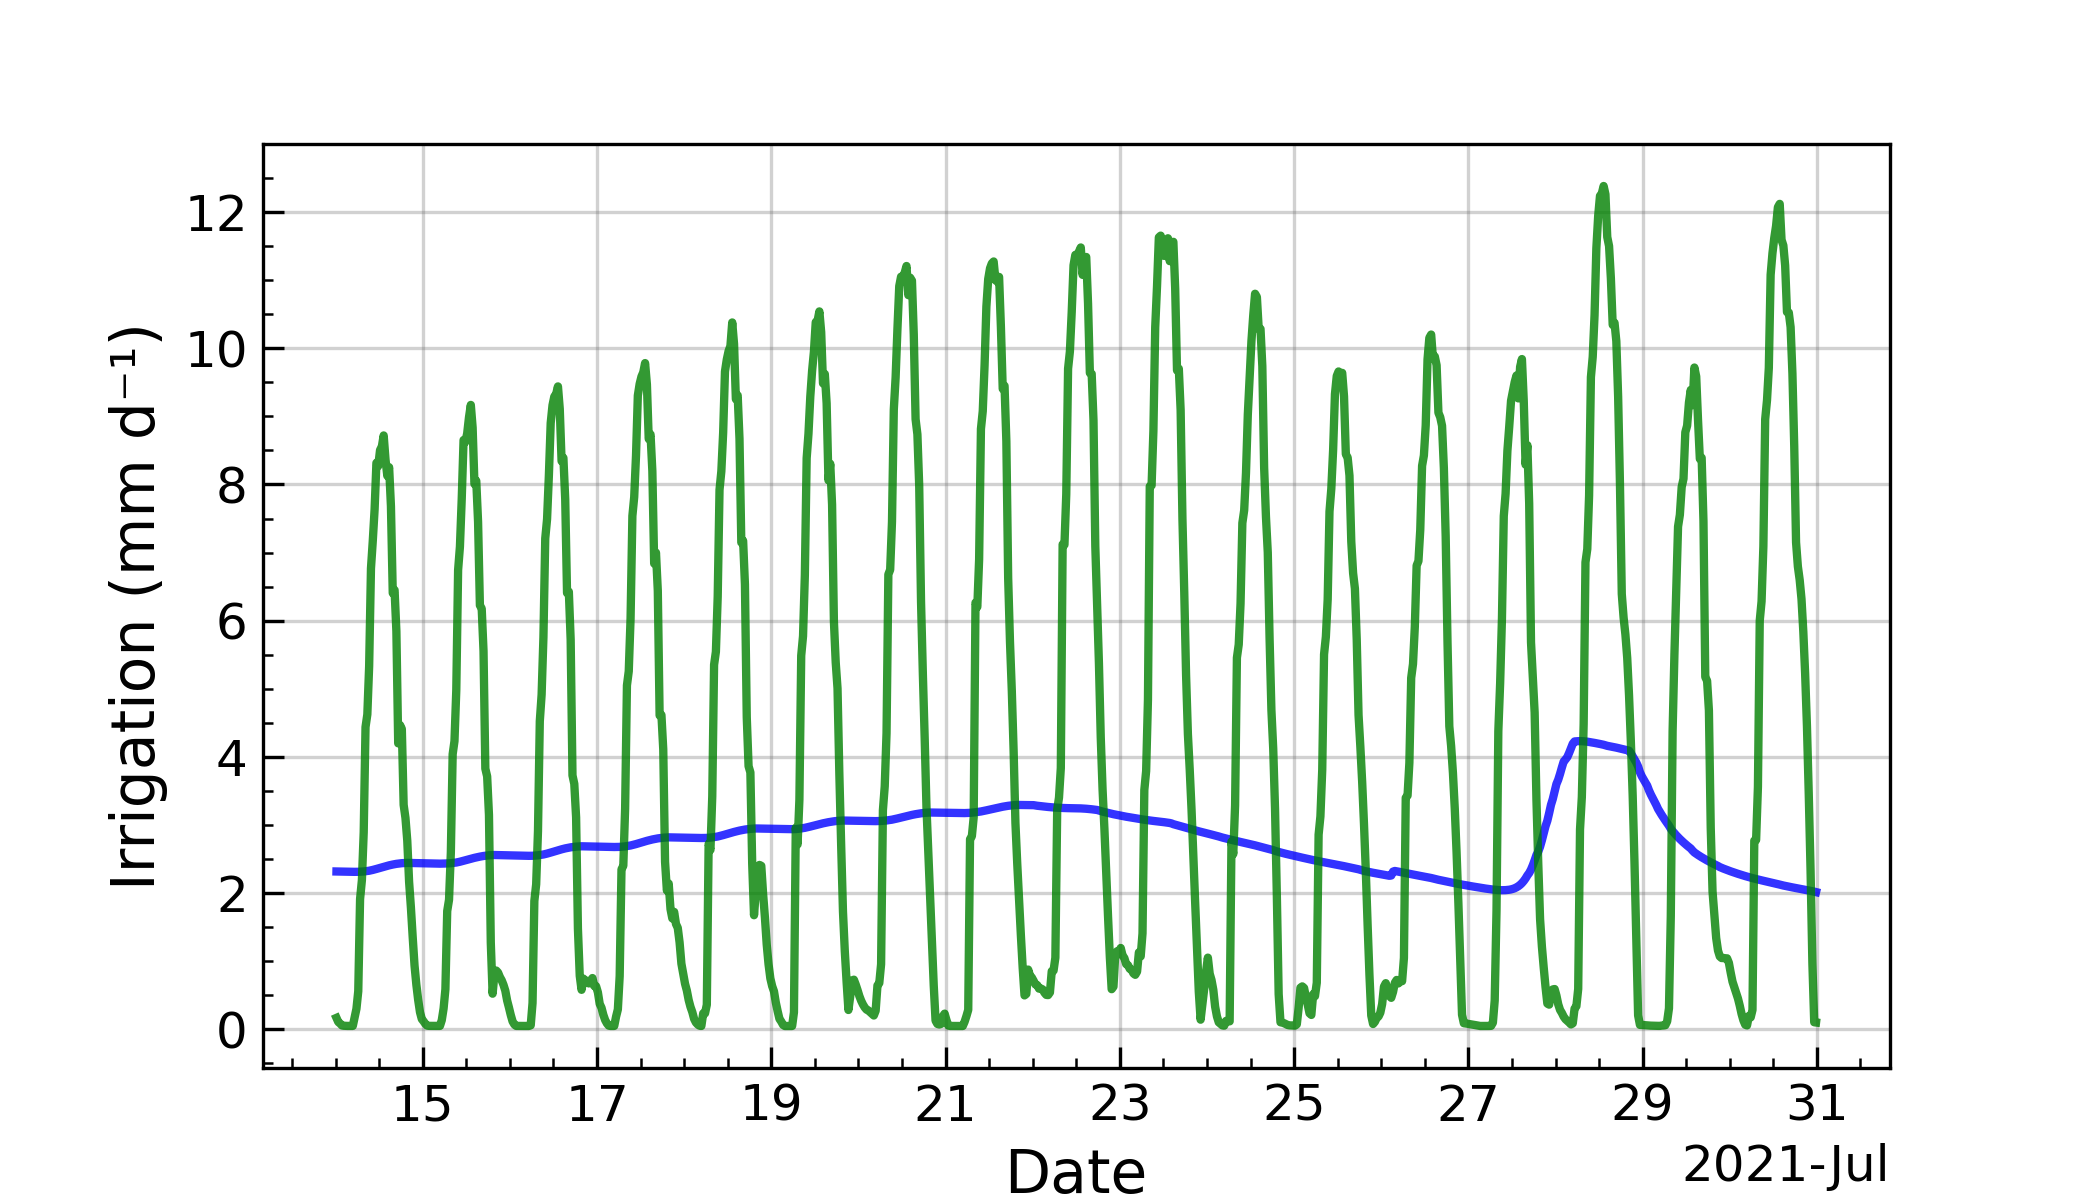
\includegraphics[width=\textwidth]{images/chap6/SOP_TS_DC/time_series_cendrosa_irrigation.png}
        \end{subfigure} &
        \begin{subfigure}[t]{0.5\textwidth}
            \caption{}
            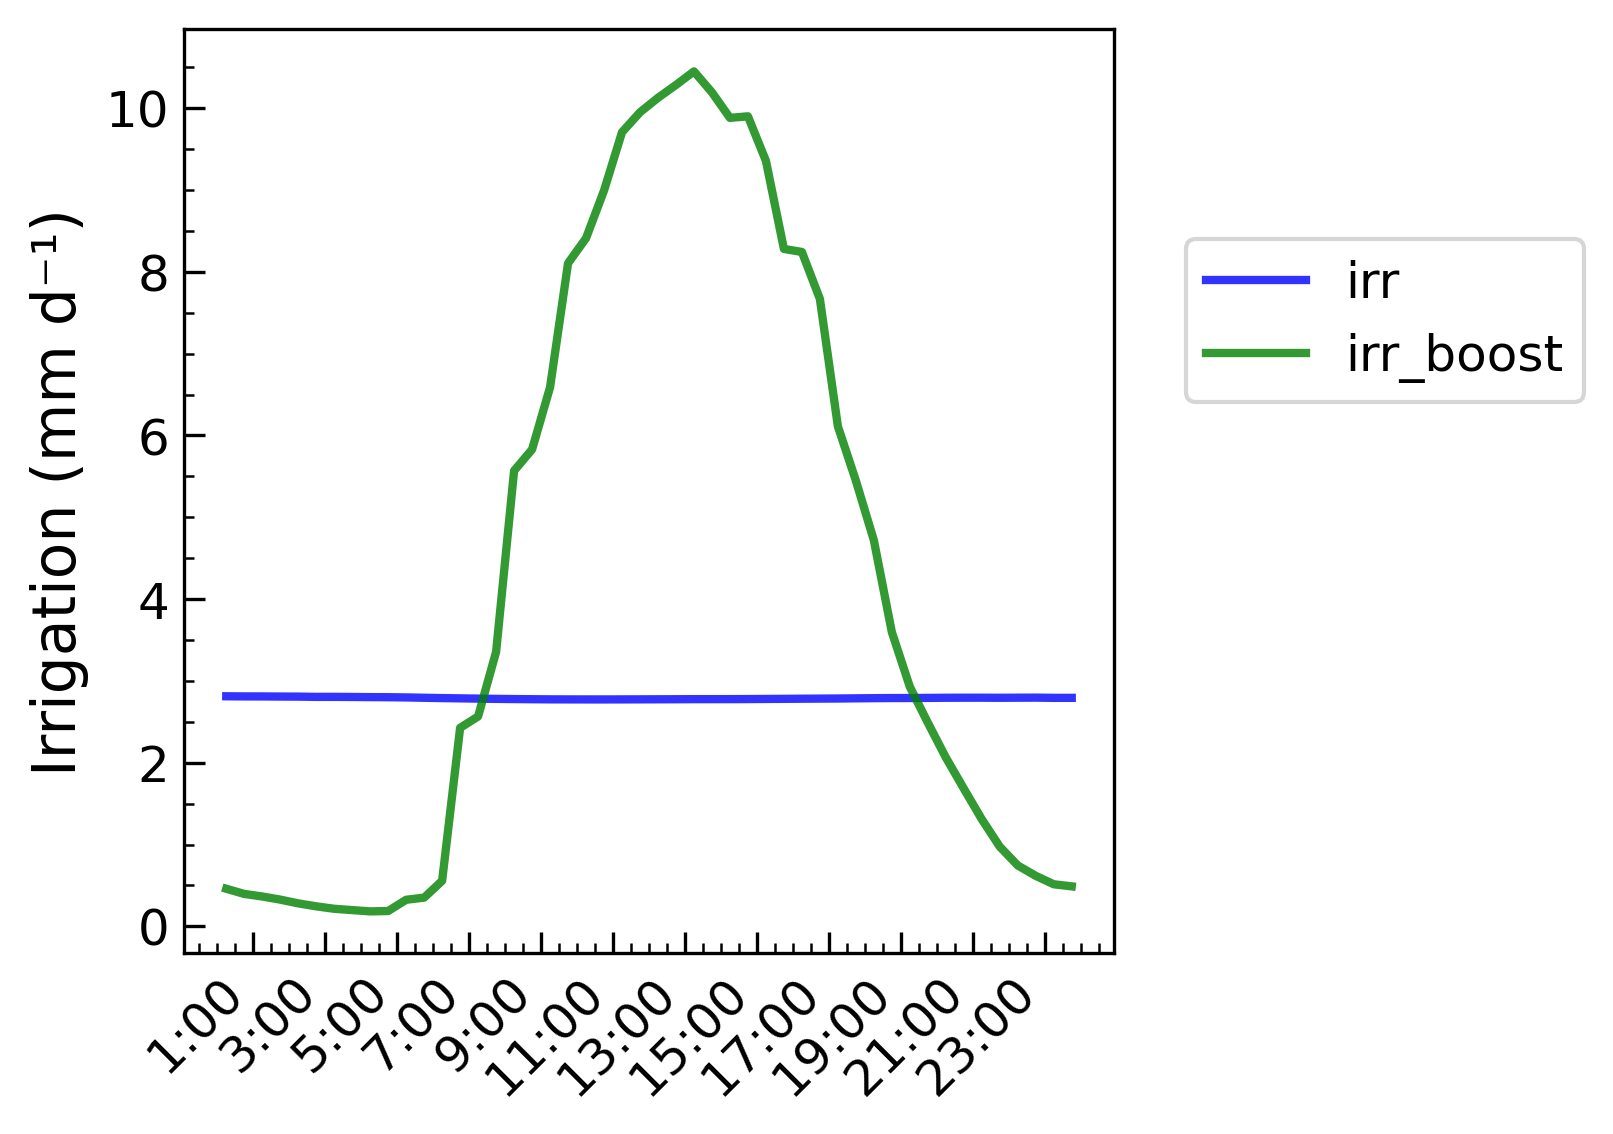
\includegraphics[width=\textwidth]{images/chap6/SOP_TS_DC/diurnal_cycle_cendrosa_irrigation.png}
        \end{subfigure}
    \end{tabular} 
    \caption{Time series and mean diurnal cycle  of irrigation simulated by ICOLMDZOR at La Cendrosa in \irr and \irrboost simulations, 14-30 July.}
    \label{fig:sop_irrigation_orchidee}
\end{figure}

Regarding available water, since this was a short simulation run (one month), very large qunatities of water were added in the three routing reservoirs at the initial state of the simulation, making a virtually inifinite volume of water available for irrigation in the LIAISE region. Obviously, this method is not realistic, nor applicable to longer climate runs, and was only used to test the limits of the irrigation scheme and explore the sensitivities of land-atmosphere interactions in a context where irrigation would be driven by the water demand rather than the supply. 
Compared to reality, this can also be seen as a way to compensate for the absence of water adduction in the ICOLMDZOR LAM simulations, a practice that is determinant in the actual supply of irrigated water in the area. 
The differences in simulated irrigation between \irr and \noirr are shown on Fig. \ref{fig:sop_irrigation_orchidee} and will later be discussed in Section \ref{sec:sop}.

\hfill

The three ICOLMDZOR LAM simulations (\noirr, \irr, \irrboost) are compared to observations and to the Meso-NH simulation from 14 to 30 July. This covers all the LIAISE SOP and allows for the stabilization of irrigation volumes in the \irrboost simulation, since no long-term spinup was conducted with this setup.
For each site, an ICOLMDZOR grid cell was selected for the comparison to observations. At Els Plans, the grid cell containing the exact site location seemd appropriate since it was a very lightly irrigated cell. however, the exact position of the La Cendrosa site was not in an intensely irrigated cell, which is why the neighbouring grid cell was selected.

%fig:sites and corresponding grid cells
\begin{figure}[hbtp]
    \centering
    \begin{tabular}{cc}
        \begin{subfigure}[t]{0.44\textwidth}
            \caption{Visible image of the LIAISE study area as seen by \textit{Sentinel-2} on 22 July 2021.}
            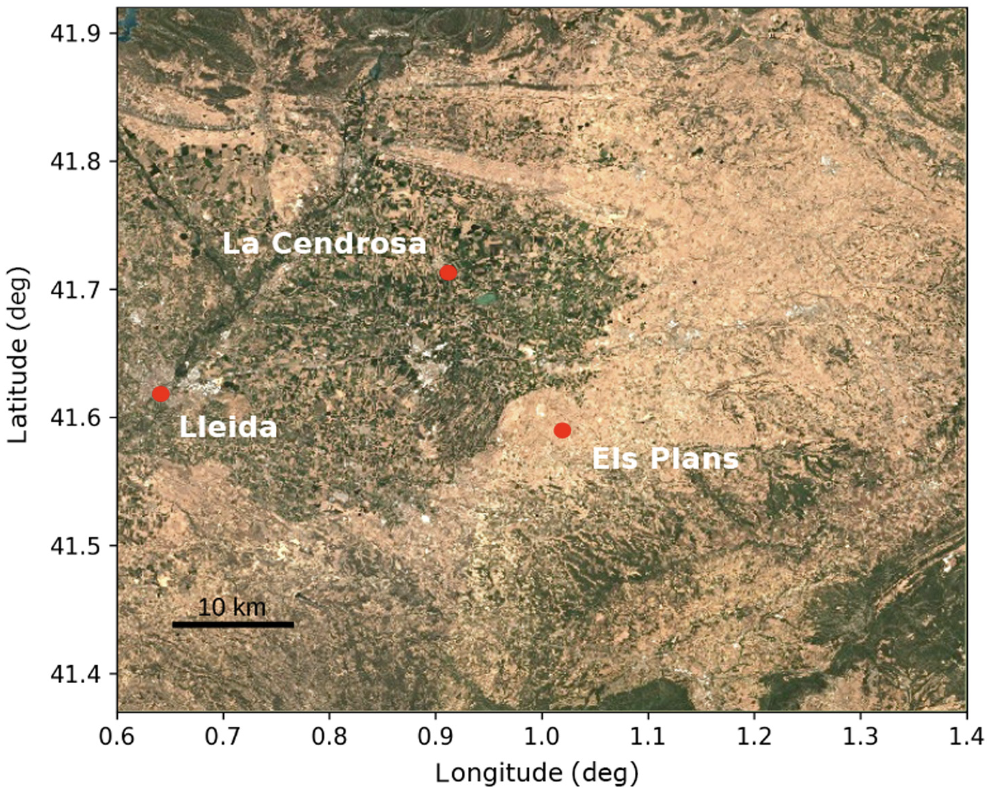
\includegraphics[width=\textwidth]{images/chap6/liaise_overview_lunel.png}
        \end{subfigure} &

        \begin{subfigure}[t]{0.5\textwidth}
            \caption{Monthly average irrigation simulated by ORCHIDEE (July 2021, \irr simulation).}
            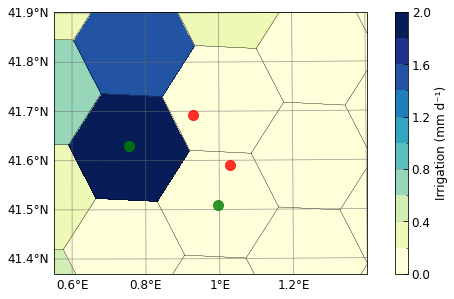
\includegraphics[width=\textwidth]{images/chap6/liaise_sites_irrig_ORC.png}
        \end{subfigure} 
    \end{tabular} 

    \begin{subfigure}[t]{0.75\textwidth}
            \caption{Average latent heat flux simulated by Meso-NH (14-30 July 2021, with irrigation). Red hexagons show the ICOLMDZOR grid cells for each site.}
            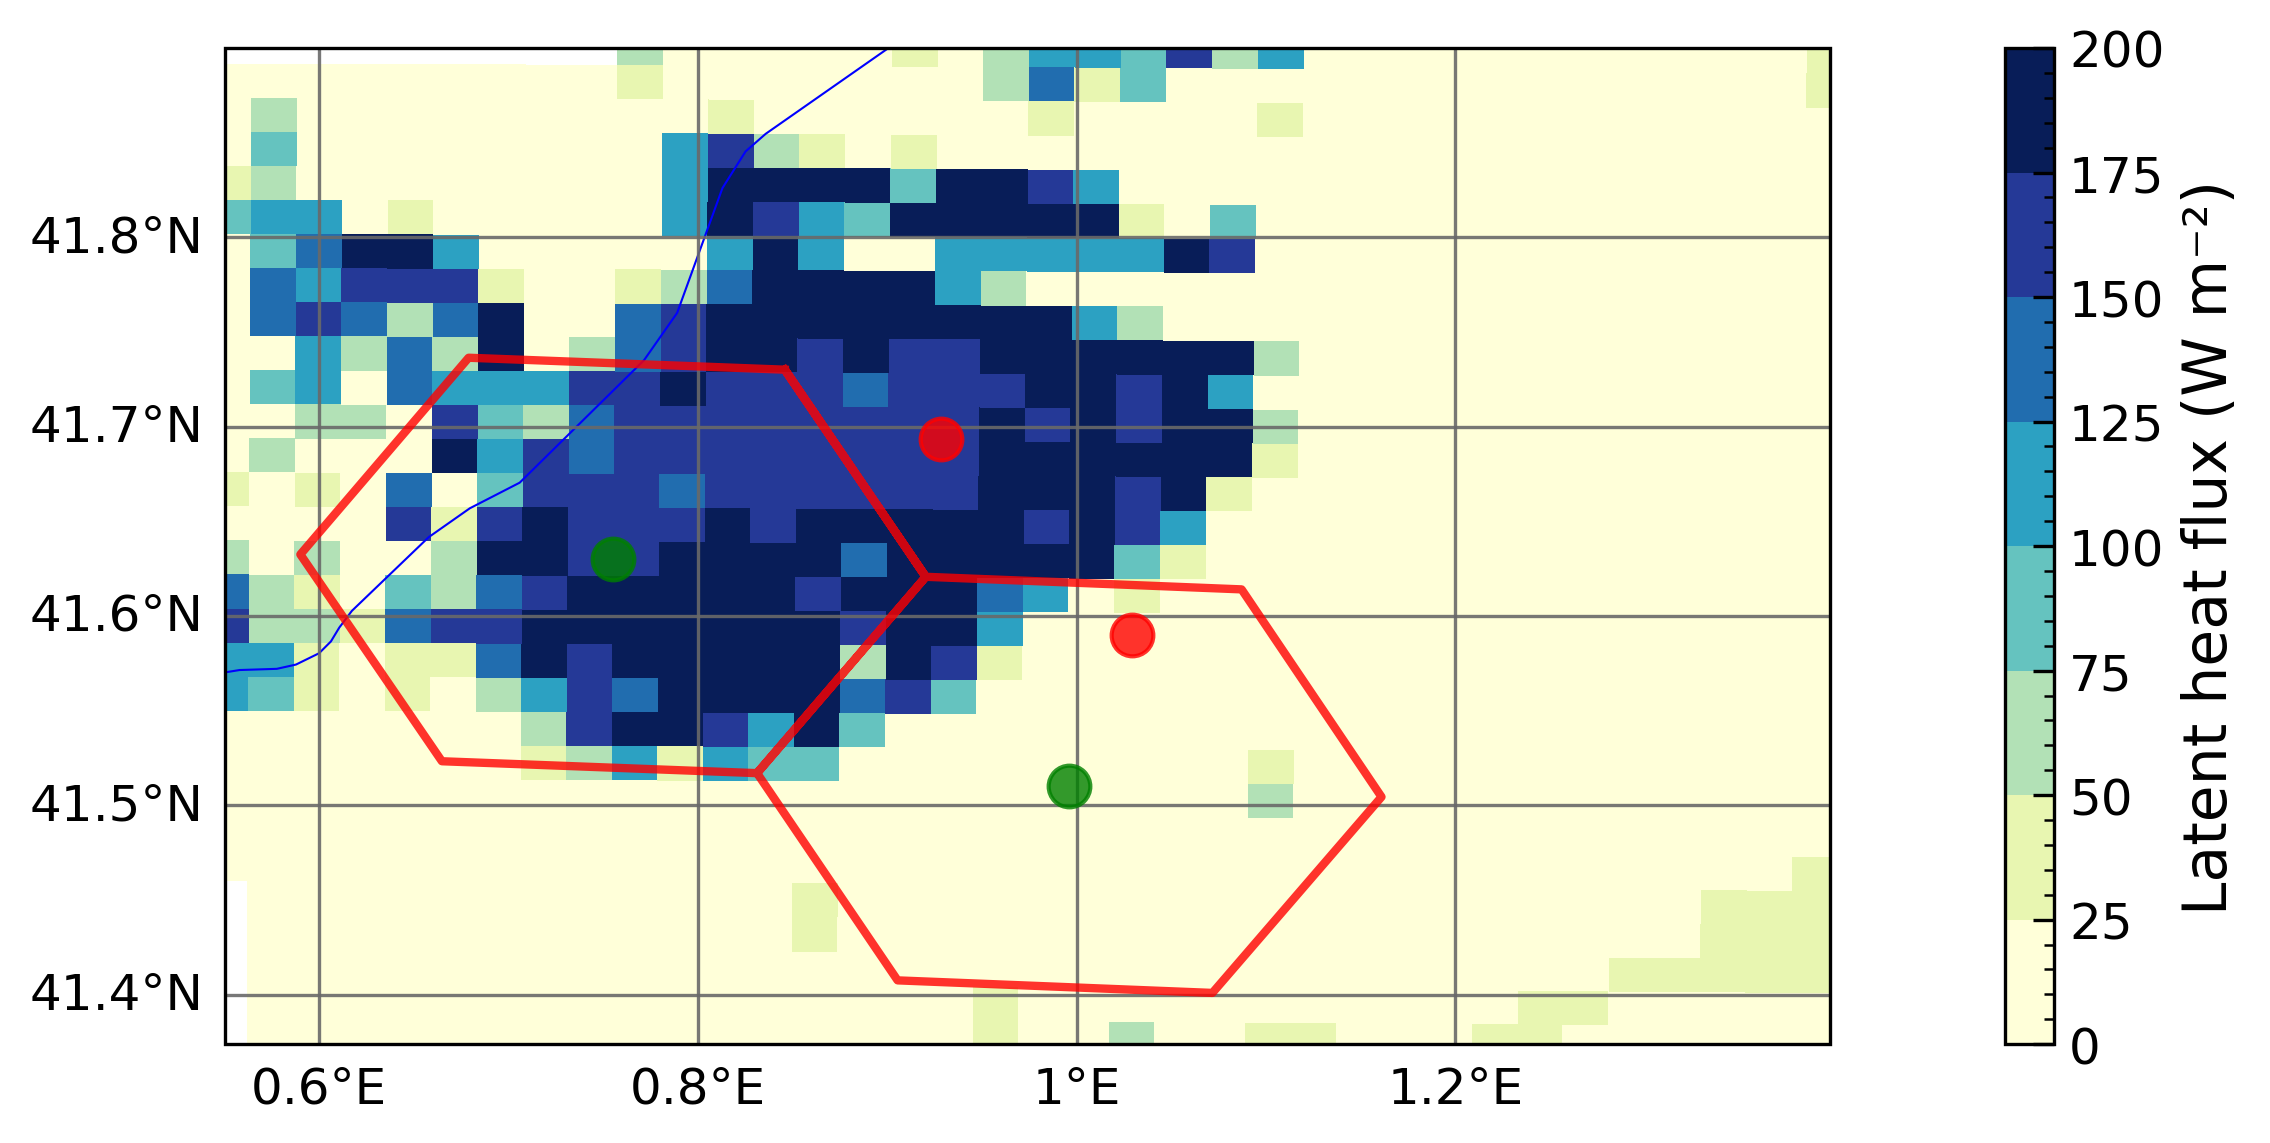
\includegraphics[width=\textwidth]{images/chap6/liaise_sites_mean_mesoNH.png}
        \end{subfigure} 
    
    \caption{Correspondance between actual location of La Cendrosa and Els Plans sites (red dots), selected ICOLMDZOR grid cells (centered on green dots), and Meso-NH grid. (a) was taken from \citet{lunel_irrigation_2024}.}
    \label{fig:liaise_sites_grid_cells}
\end{figure}

Comparison to the Meso-NH simulations was performed using two values for each site. 
The first one, referred to as \mesoexact, takes the variables from the exact grid cell corresponding to the site location based on the coordinates of the site, as done in \citet{lunel_irrigation_2024}. 
The second, referred to as \mesomean, is an aggregation of all the Meso-NH grid cells contained into the selected ICOLMDZOR grid cell for each site. The mean value is shown, as well as an envelope encompassing the 25th and 75th percentiles, when it is appropriate.
On Fig. \ref{fig:liaise_sites_grid_cells}c, the two hexagonal ICOLMDZOR grid cells are drawn upon the average latent heat flux simulated by Meso-NH. It can already be noticed that within the grid cell for La Cendrosa, there are some Meso-NH grid cells with very low values of ET, and that in the grid cell for Els Plans, there are some Meso-NH grid cells which fall into the irrigated zone and exhibit high ET. This will have an influence on the \mesomean values and on the spread of Meso-NH surface variables within one ICOLMDZOR grid cell. 
%option:mesoMean is not meant to be more representative of the obs than mesoExact, but to bring information on heterogeneity within one ICOLMDZOR grid cell

\section{Near-surface variables over the SOP}
\label{sec:sop}

Here, surface variables simulated by ICOLMDZOR and Meso-NH are compared to the observations on both sites from 14 to 30 July, the span of the Meso-NH simulation, which corresponds to the LIAISE SOP.

\subsubsection*{La Cendrosa}
At La Cendrosa (Fig. \ref{fig:cendrosa_surfacevars}), observed turbulent fluxes (in black) exhibit a clear diurnal cycle driven by insolation, with a maximum value between 12 and 13UTC.
In the \noirr simulation (in red), ICOLMDZOR simulates a negligible latent heat flux (Fig. \ref{fig:cendrosa_surfacevars}b) and largely overestimates the sensible heat flux (+300\% at 12UTC on Fig. \ref{fig:cendrosa_surfacevars}d). 
These major biases are partly improved in the \irr simulation (in blue), showing that additional soil moisture brought by irrigation can really improve turbulent fluxes. However, latent heat flux simulated in \irr follows a good trajectory from 5UTC to 9UTC but then drops and remains largely underestimated until the evening. This is due to a failure of the irrigation parametrization which cannot sustain the irrigation demand throughout the day since the routing reservoirs cannot provide sufficient water volumes for withdrawals. In \irr, the irrigation volume is nearly constant throughout the day (Fig. \ref{fig:sop_irrigation_orchidee}) because the soil moisture deficit is always large but the water withdrawals are capped by available water.
In the \irrboost sensitivity experiment (in green), there is an effectively infinite supply of water in the reservoirs, which allows irrigation to follow a structured diurnal cycle (Fig. \ref{fig:sop_irrigation_orchidee}) and removes the constraint of soil moisture on ET. Both turbulent fluxes follow a diurnal cycle that is consistent with observations, although a small underestimation of latent heat flux and an overestimation of sensible heat flux remain compared to the observations. 
However, the turbulent fluxes in \irrboost are very close to those of \mesomean (in yellow, with the envelope representing the 25th and 75th percentiles of the distribution), suggesting that ICOLMDZOR correctly represents the average fluxes over the grid cell, which does not only include intensely irrigated areas.
It can be noted here that \mesoexact (in purple), corresponding to the exact Meso-NH grid cell of the observation site, overestimates latent heat flux on average over the period. This is mostly due to the beginning of the SOP, where the alfalfa crops at La Cendrosa were still freshly cut and had not recovered their original size, LAI and transpiration levels.

The diurnal cycle of 2-meter temperature is also driven by insolation but its shape is slightly shifted with a peak in the afternoon around 4UTC (Fig. \ref{fig:cendrosa_surfacevars}f). Figure \ref{fig:cendrosa_surfacevars}e shows that temperatures were consistently rising throughout the SOP, from 15 to 22 July, and that this evolution is well captured by ICOLMDZOR and Meso-NH.
On average over the SOP, all simulations exhibit a warm bias, of at least 1.5° at night, where \mesoexact is closer to ICOLMDZOR than to observations, and of varying amplitude during the day. The \irr simulation has the strongest warm bias, which is consistent with the simulated turbulent fluxes, and this bias is slightly reduced in \irr. In \irrboost, it is largely improved, with a peak temperature 2°C lower than \irr, and simulated values that follow \mesomean throughout most of the day. In the evening, \irrboost even falls closer to observed values than to \mesomean, which suggests that if turbulent fluxes are correctly simulated, the structural nighttime warm bias is smaller in ICOLMDZOR than in Meso-NH.

The diurnal cycle for 2-meter specific humidity is less structured than turbulent fluxes or temperatures.
On Fig. \ref{fig:cendrosa_surfacevars}h, Meso-NH appears to present a dry bias a night, with an underestimation of specific humidity in \mesoexact as strong as in \mesomean. With ICOLMDZOR, a similar bias is present in \noirr, but it is absent in \irr and \irrboost, likely thanks to local ET enabled by irrigation.
In daytime, \mesoexact matches observed values from 8UTC to 18UTC, and \mesomean follows a similar structure through the diurnal cycle. 
ICOLMDZOR, on the contrary, presents an incorrect diurnal cycle of specific humidity, with an extensive drying in daytime. The strength of this drying is largest in \noirr but \irrboost still falls below the values of \mesomean, at the limit of the 25th percentile. 
The differences between ICOLMDZOR and observed values increase largely from 20 July, where humidity drops in the simulations but not in reality or in Meso-NH simulation (Fig. \ref{fig:cendrosa_surfacevars}g).
This shows that in certain daytime conditions, increasing ET by accounting for irrigation is not sufficient to simulate a realistic 2-meter specific humidity. In particular, incorrect advection terms and surface wind can neutralise the effect of this local improvement of land-atmosphere interactions.

This hypothesis is corroborated by the 10-meter wind regime at La Cendrosa (Fig. \ref{fig:bothsites_wind}a-d), which is quite well structured in the beginning of the SOP with low wind speeds, but shows important variations in direction and an increased wind speed from 20 July. ICOLMDZOR seems to be capturing the variations quite well until 19 July but clearly misses part of the regime changes afterwards. This can clearly lead to a poor representation of advection terms over a day, failing to represent moisture inputs from the more humid Pyrnees or fro the Mediterranean sea.
On average over the SOP, \mesoexact follows observations closely, and the diurnal cycle simulated by ICOLMDZOR has the same structure as \mesomean, particularly for wind direction.
Irrigation only has an impact on the 10-meter wind speed: in \noirr it is overestimated, and that bias is partly reduced in \irr and \irrboost. This was expected since in the presence of irrigation, the vegetation is more developed and LAI is larger, leading to a larger surface drag and therefore lower surface wind speed. 
Wind direction is not impacted by irrigation (red, blue and green lines overlap in Fig. \ref{fig:bothsites_wind}d), which was also expected since only a few grid cells are intensely irrigated in the region, which limits the possibilities of influencing the dynamics of the LAM.

%fig : Cendrosa turbulent fluxes + t2m, q2m
\begin{figure}[t]
    \centering
    \begin{tabular}{cc}
        \begin{subfigure}[t]{0.5\textwidth}
            \caption{Latent heat flux (La Cendrosa)}
            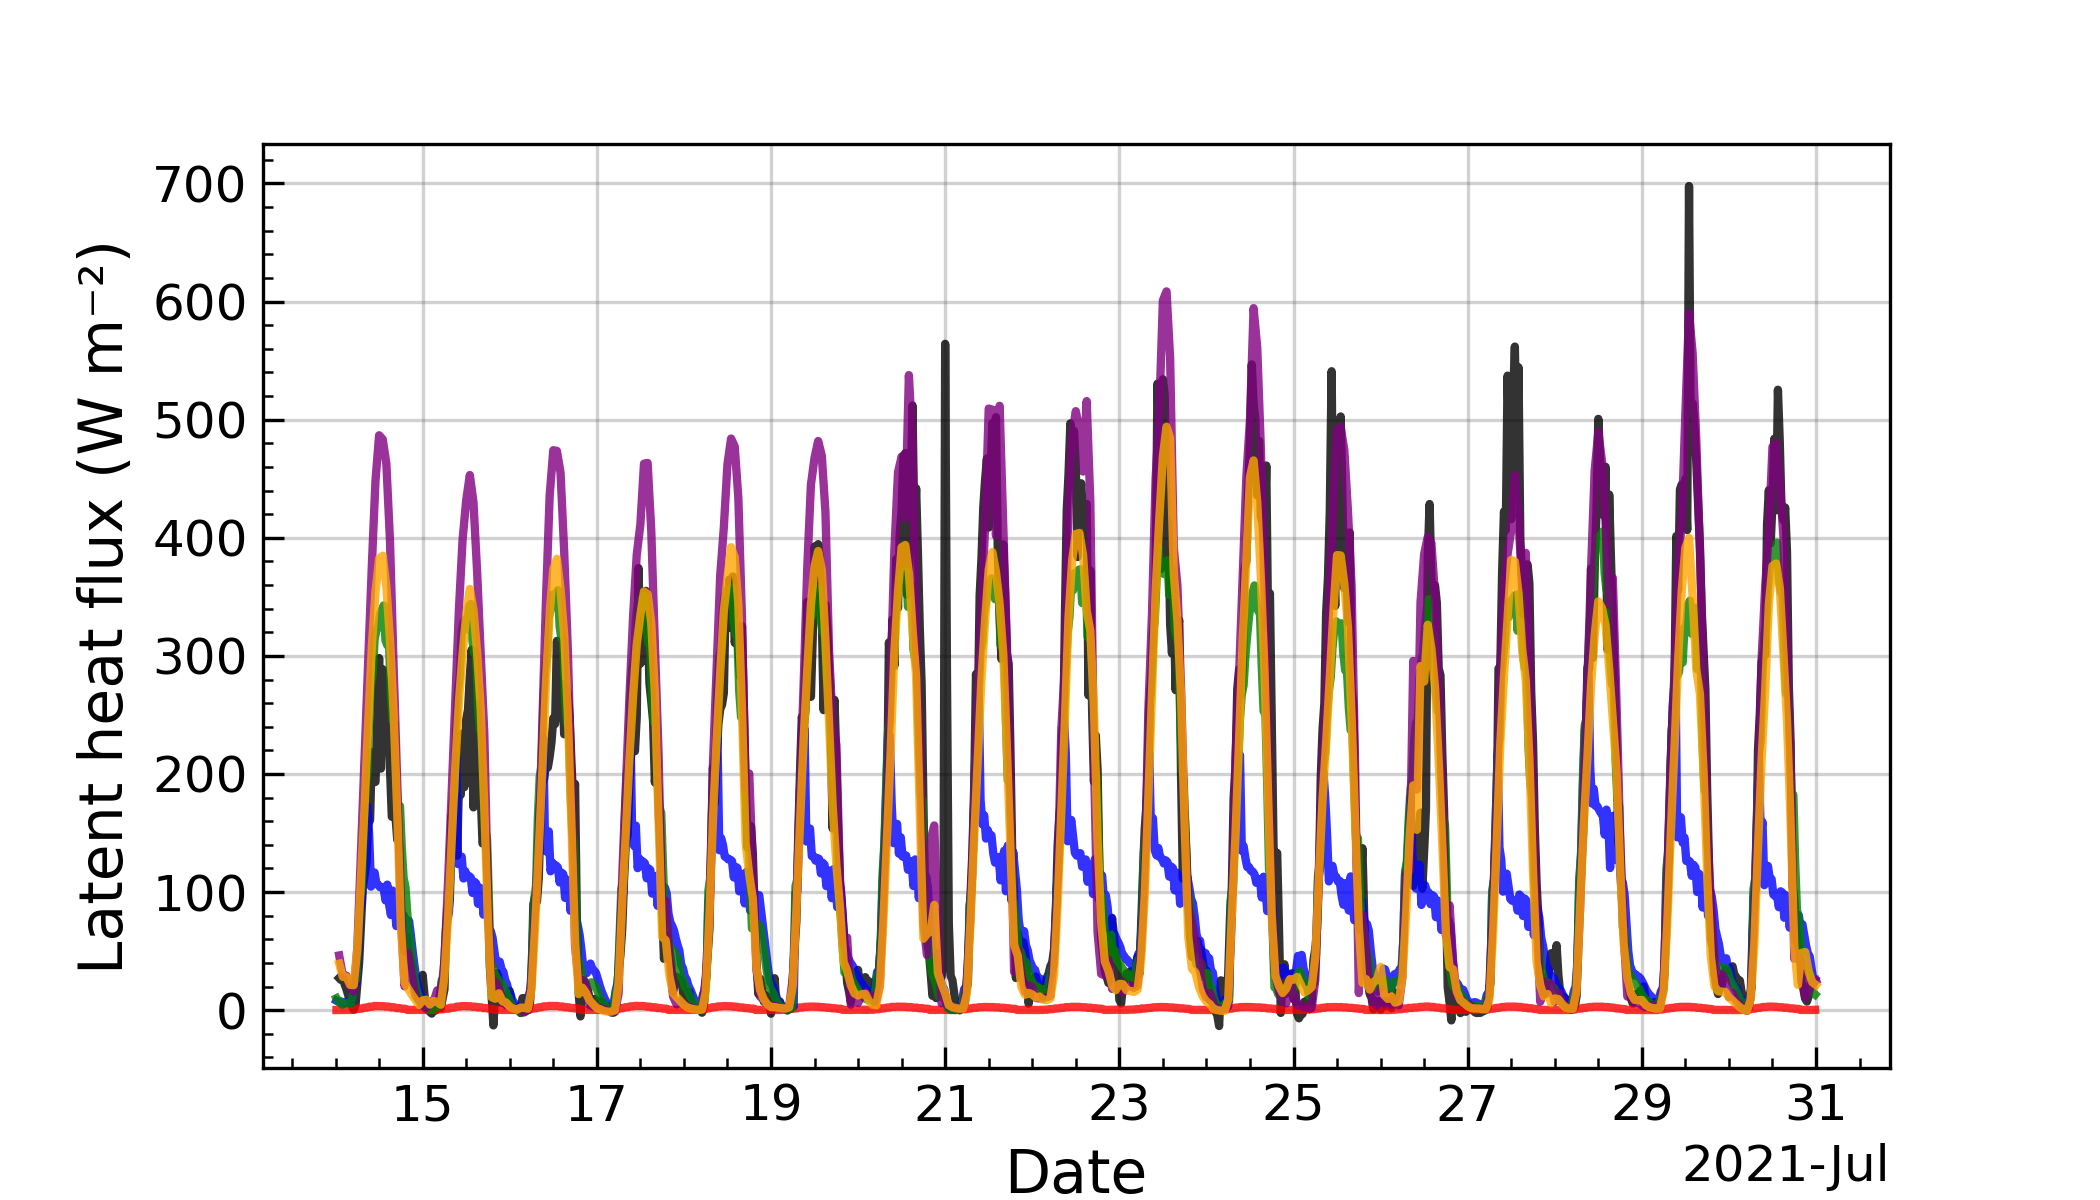
\includegraphics[width=\textwidth]{images/chap6/SOP_TS_DC/time_series_cendrosa_flat.png}
        \end{subfigure} &
        \begin{subfigure}[t]{0.5\textwidth}
            \caption{Mean diurnal cycle of latent heat flux\\(14-30 July - La Cendrosa)}
            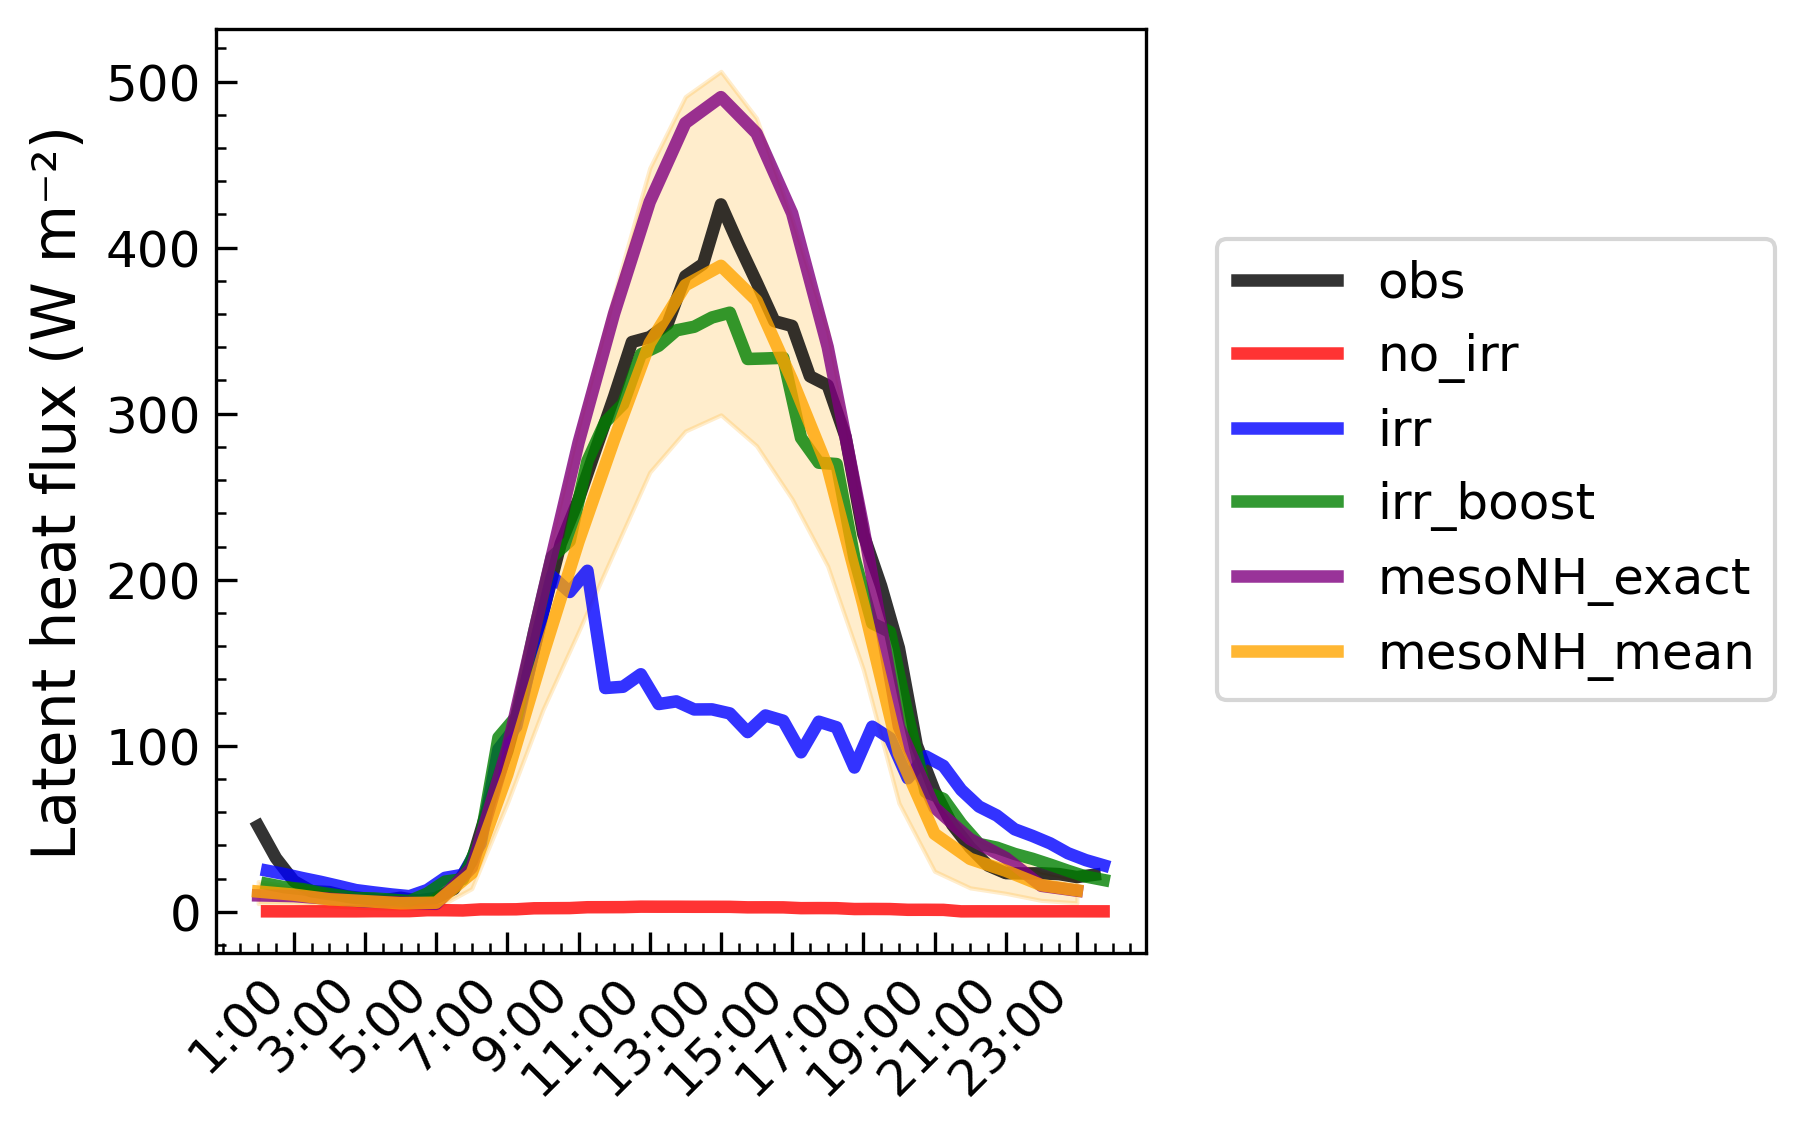
\includegraphics[width=\textwidth]{images/chap6/SOP_TS_DC/diurnal_cycle_cendrosa_flat.png}
        \end{subfigure} \\
        \begin{subfigure}[t]{0.5\textwidth}
            \caption{Sensible heat flux (La Cendrosa)}
            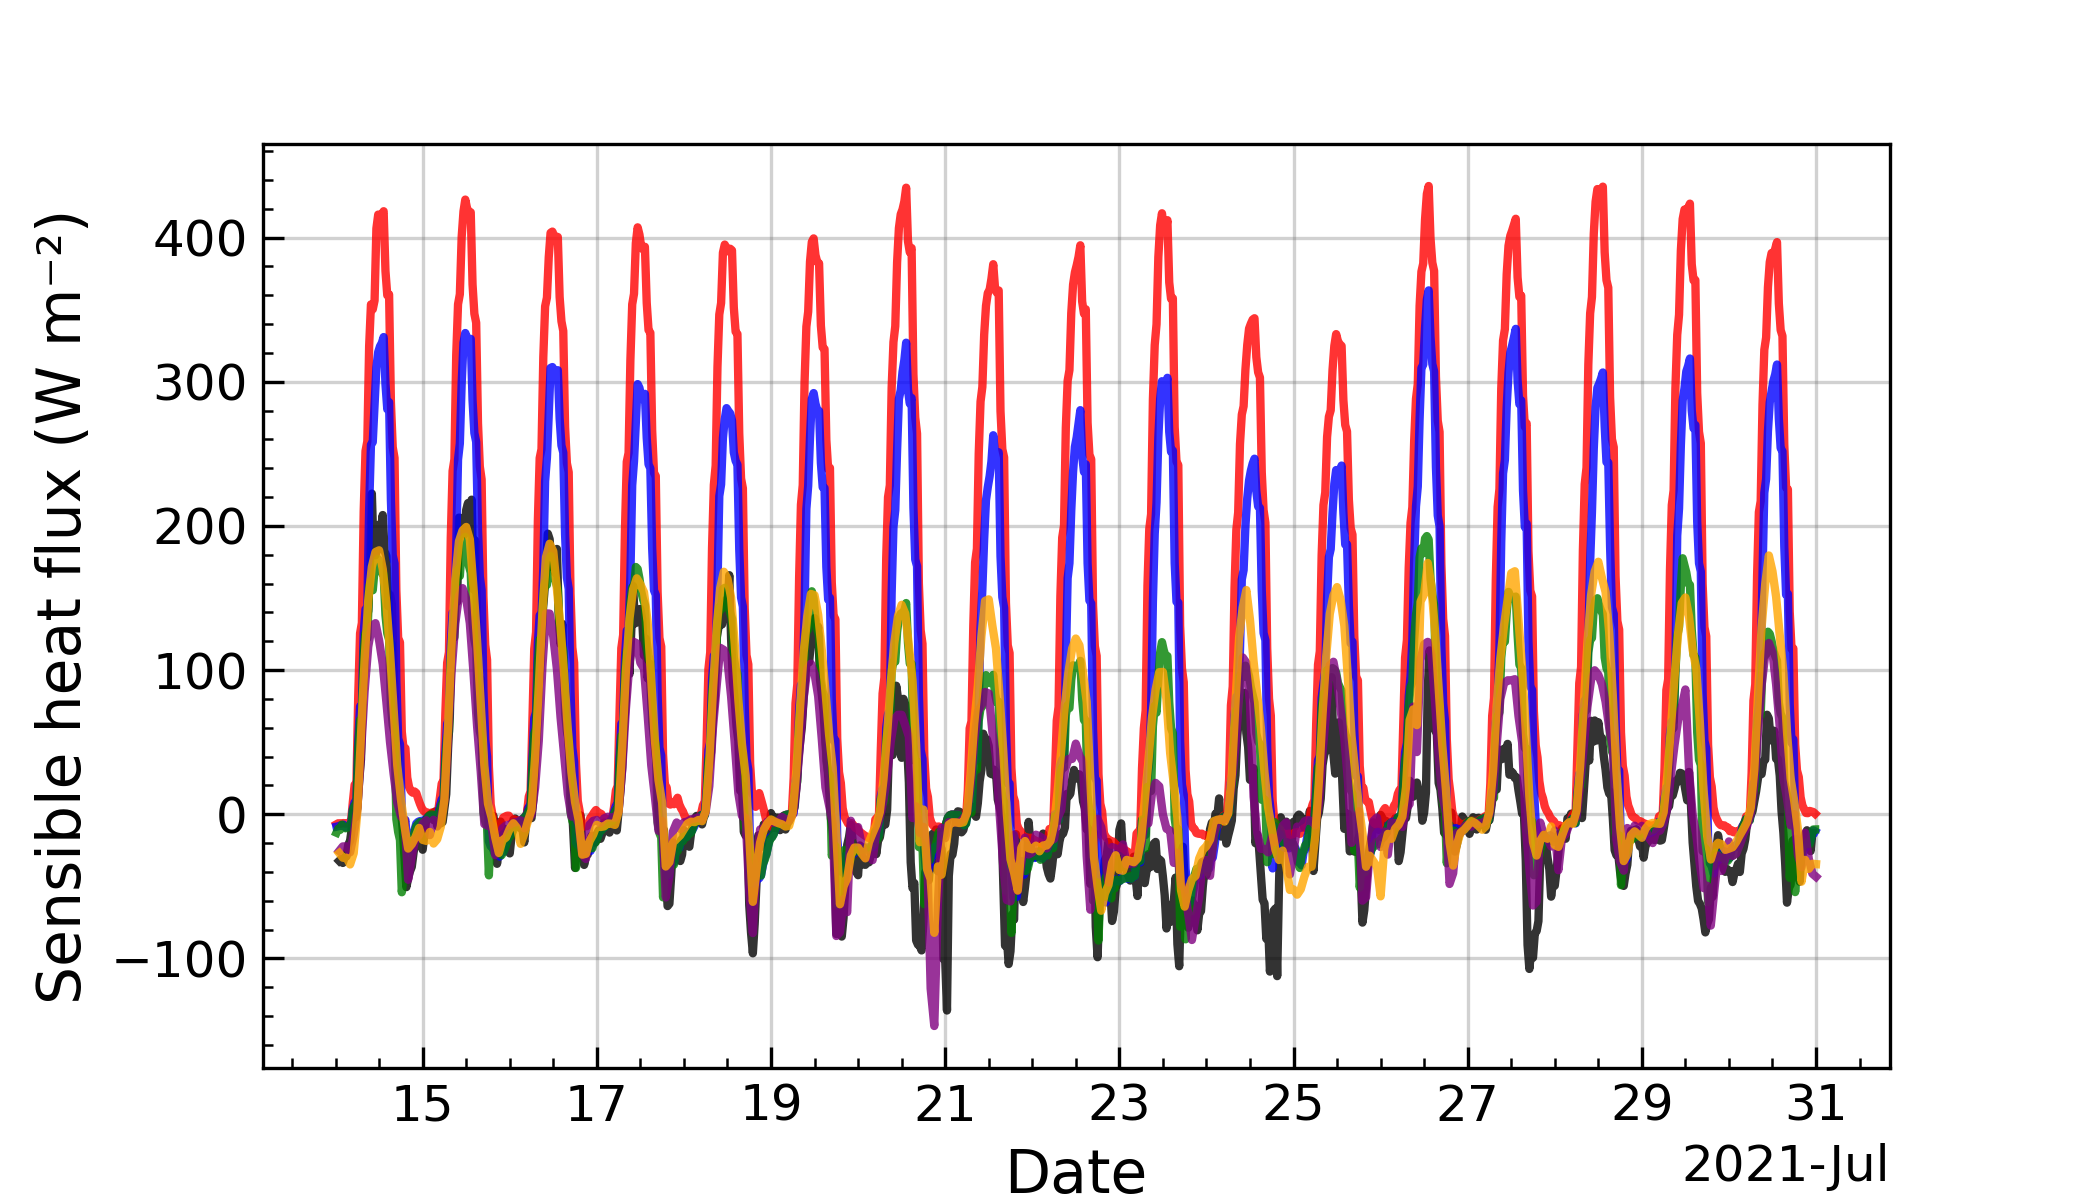
\includegraphics[width=\textwidth]{images/chap6/SOP_TS_DC/time_series_cendrosa_sens.png}
        \end{subfigure} &
        \begin{subfigure}[t]{0.5\textwidth}
            \caption{Mean diurnal cycle of sensible heat flux\\(14-30 July - La Cendrosa)}
            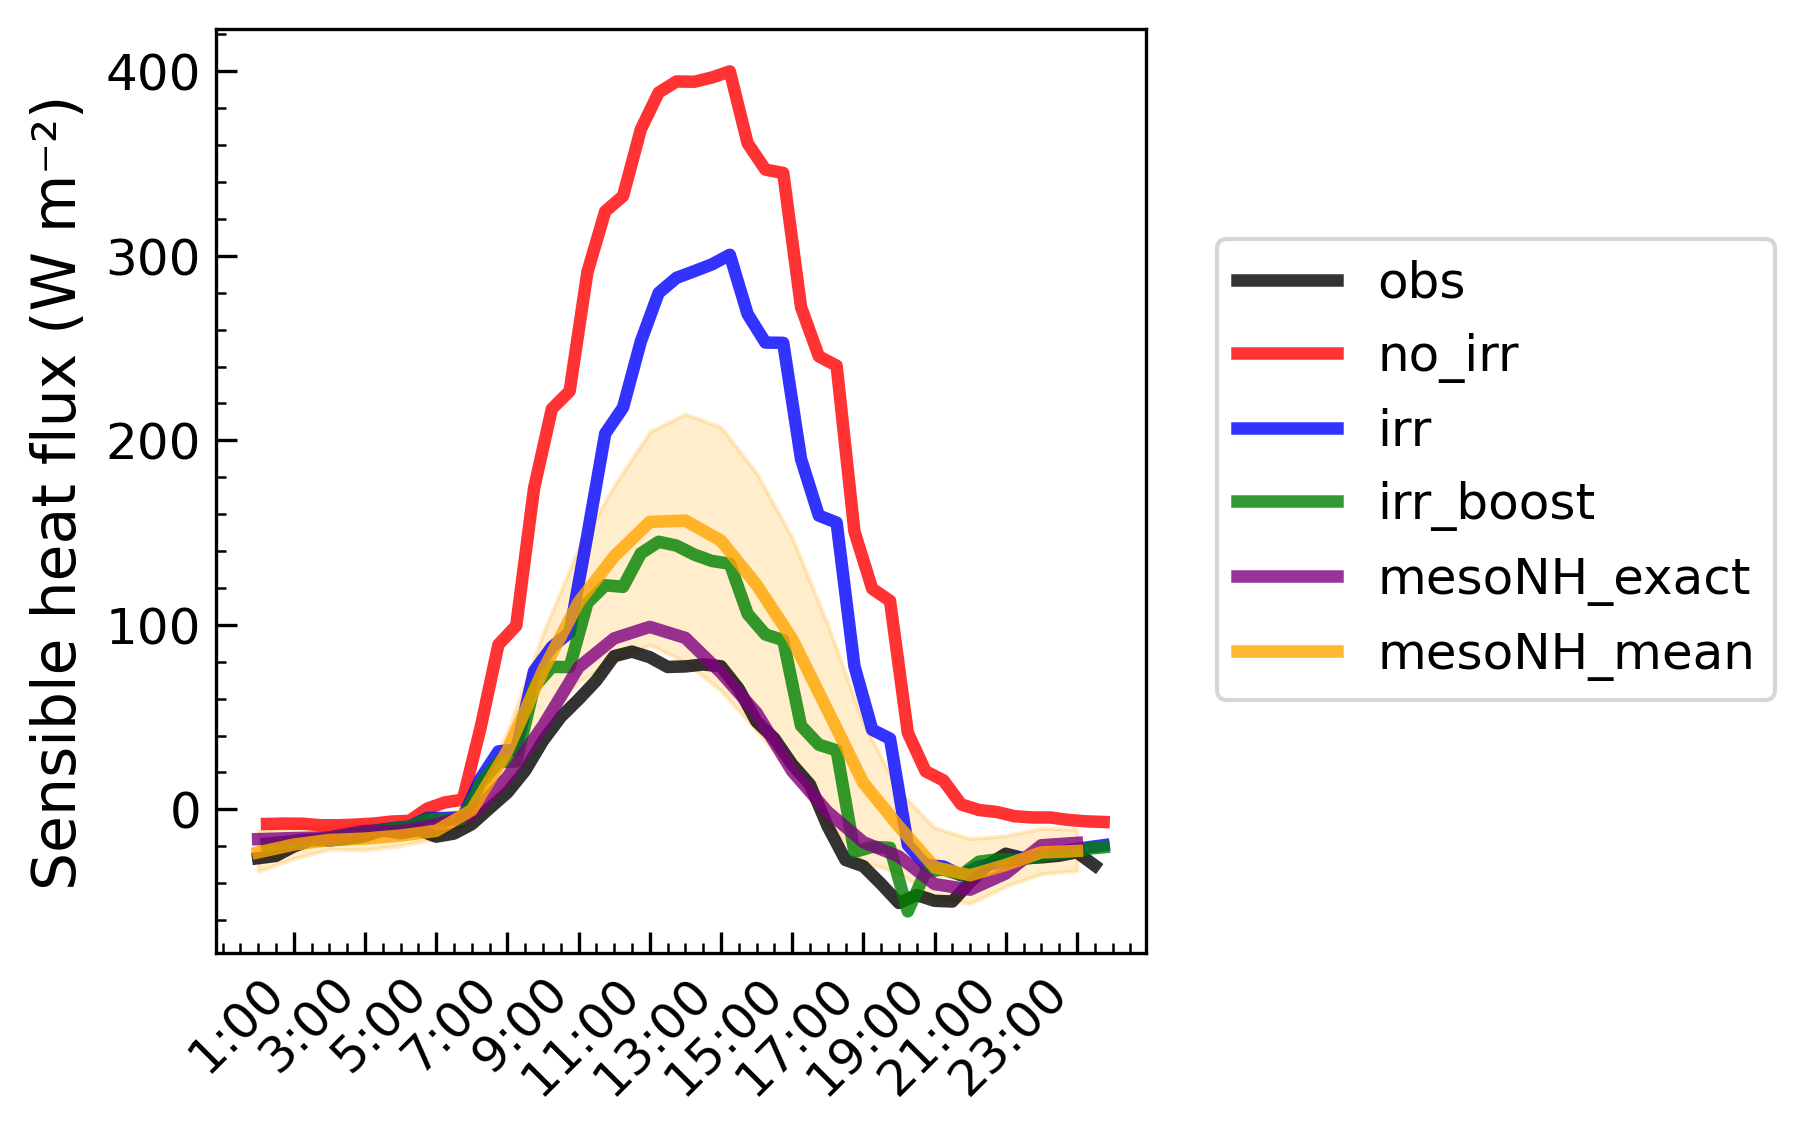
\includegraphics[width=\textwidth]{images/chap6/SOP_TS_DC/diurnal_cycle_cendrosa_sens.png}
        \end{subfigure} \\
        \begin{subfigure}[t]{0.5\textwidth}
            \caption{2-meter temperature (La Cendrosa)}
            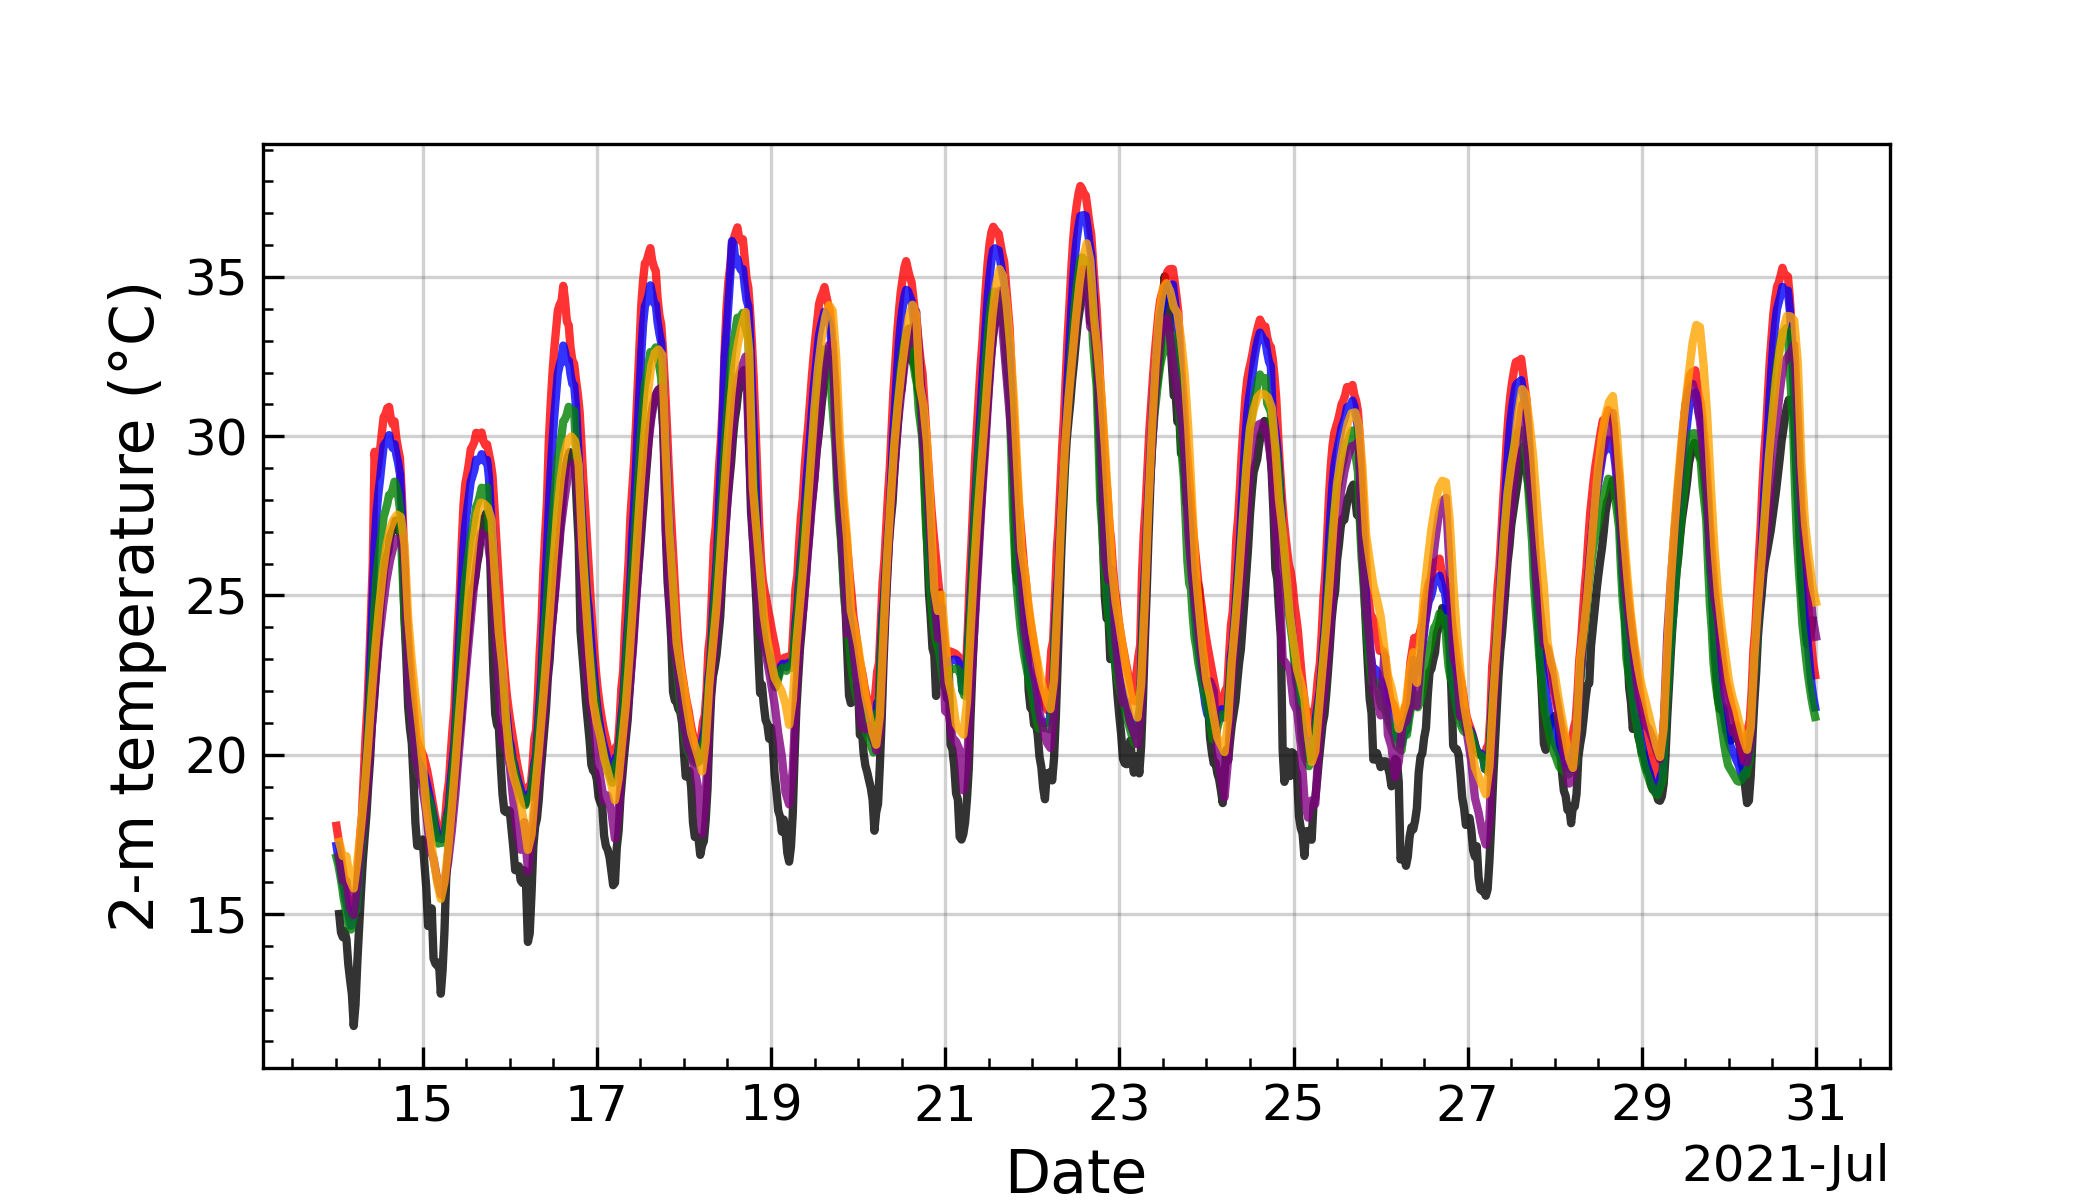
\includegraphics[width=\textwidth]{images/chap6/SOP_TS_DC/time_series_cendrosa_t2m.png}
        \end{subfigure} &
        \begin{subfigure}[t]{0.5\textwidth}
            \caption{Mean diurnal cycle of 2-meter temperature\\(14-30 July - La Cendrosa)}
            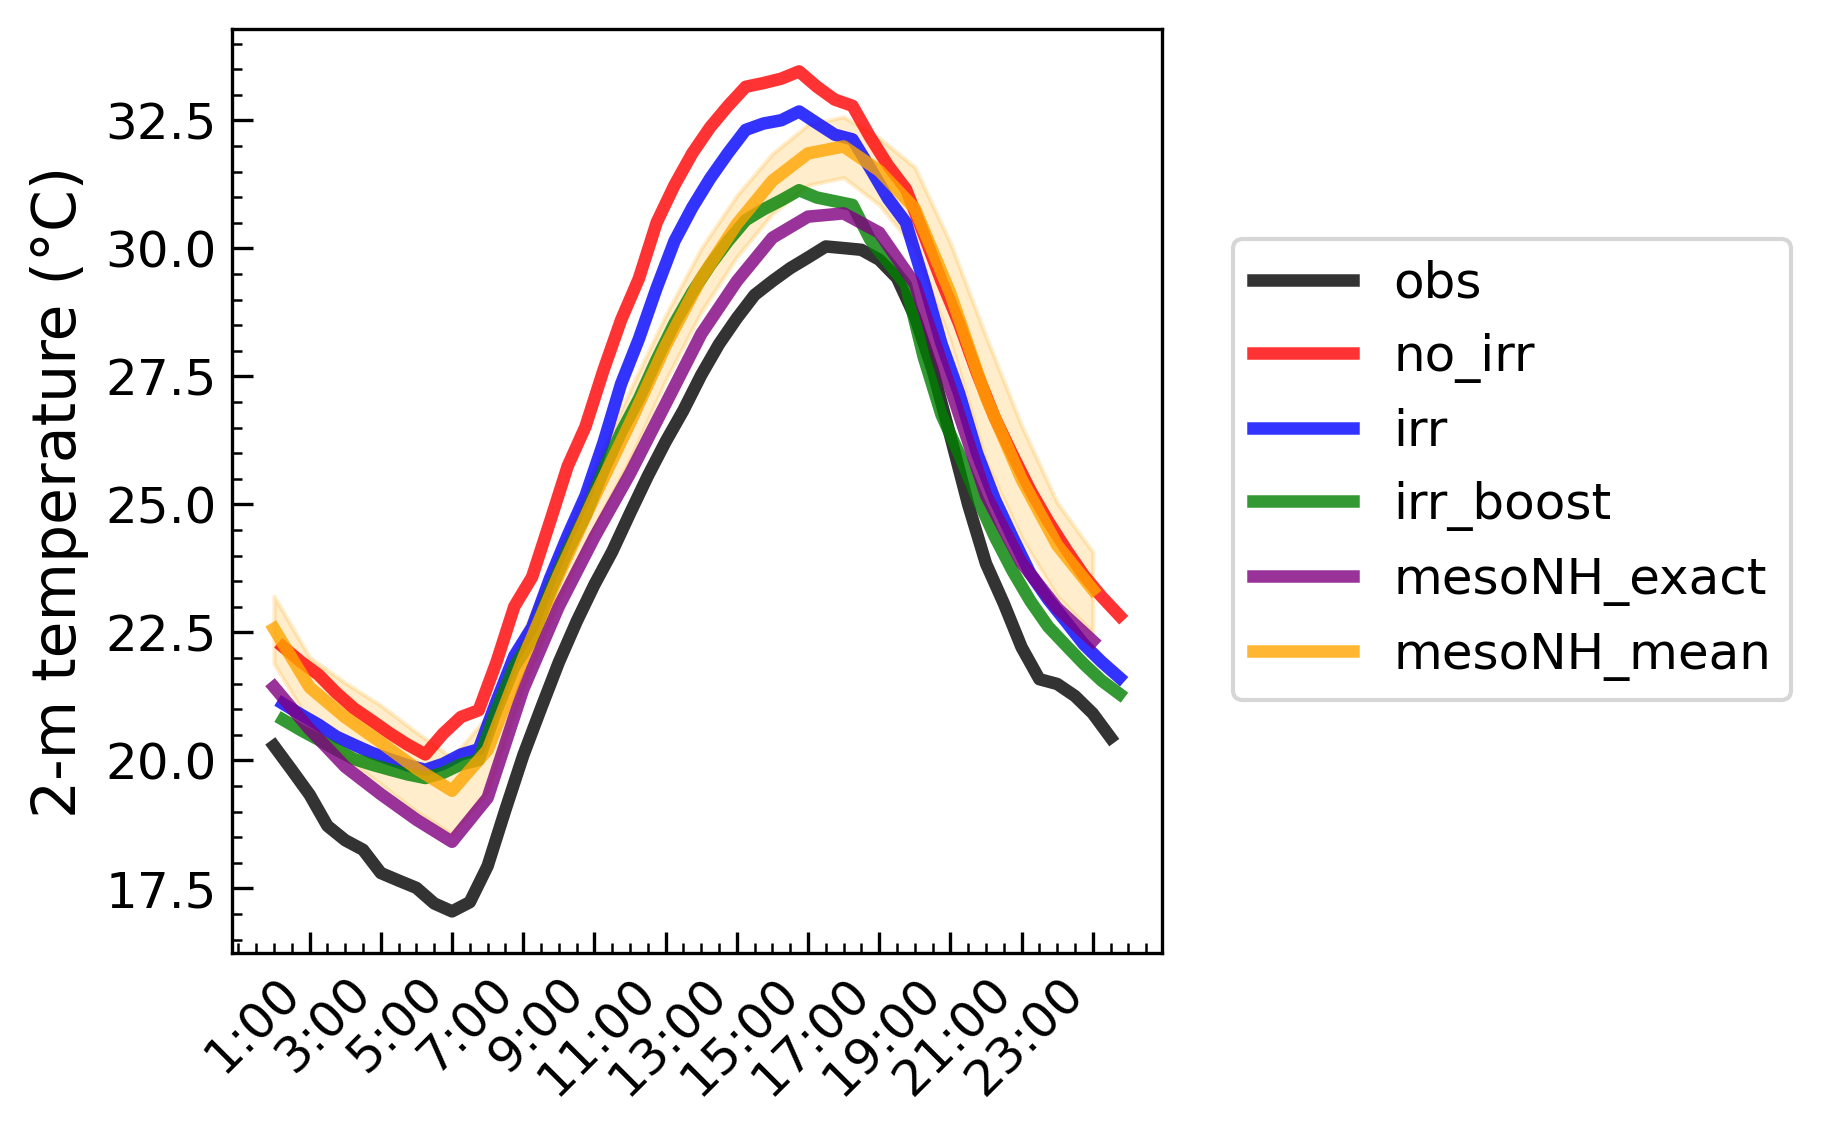
\includegraphics[width=\textwidth]{images/chap6/SOP_TS_DC/diurnal_cycle_cendrosa_t2m.png}
        \end{subfigure} \\
        \begin{subfigure}[t]{0.5\textwidth}
            \caption{2-meter specific humidity (La Cendrosa)}
            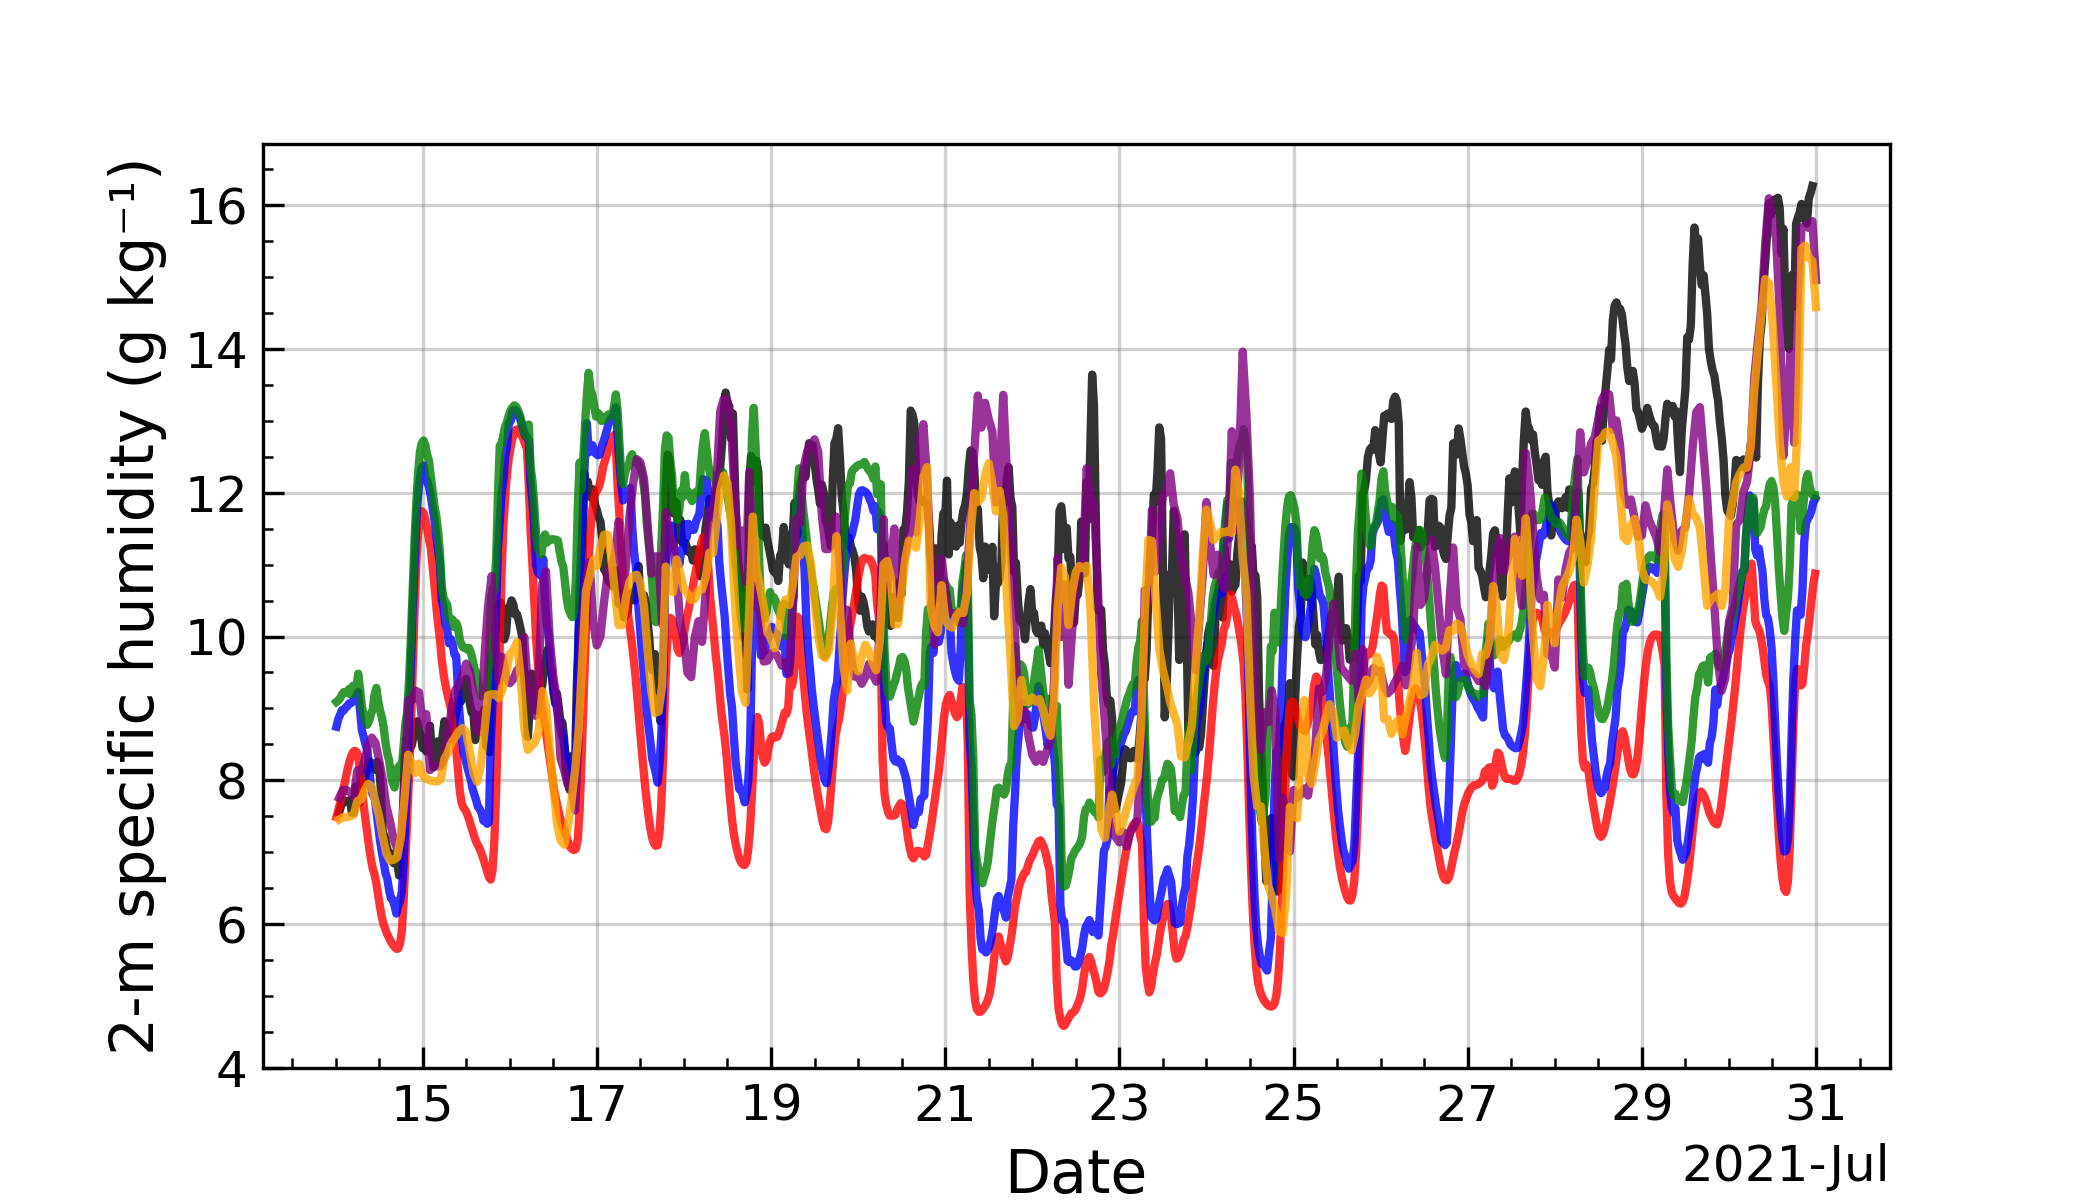
\includegraphics[width=\textwidth]{images/chap6/SOP_TS_DC/time_series_cendrosa_q2m.png}
        \end{subfigure} &
        \begin{subfigure}[t]{0.5\textwidth}
            \caption{Mean diurnal cycle of 2-meter specific humidity\\(14-30 July - La Cendrosa)}
            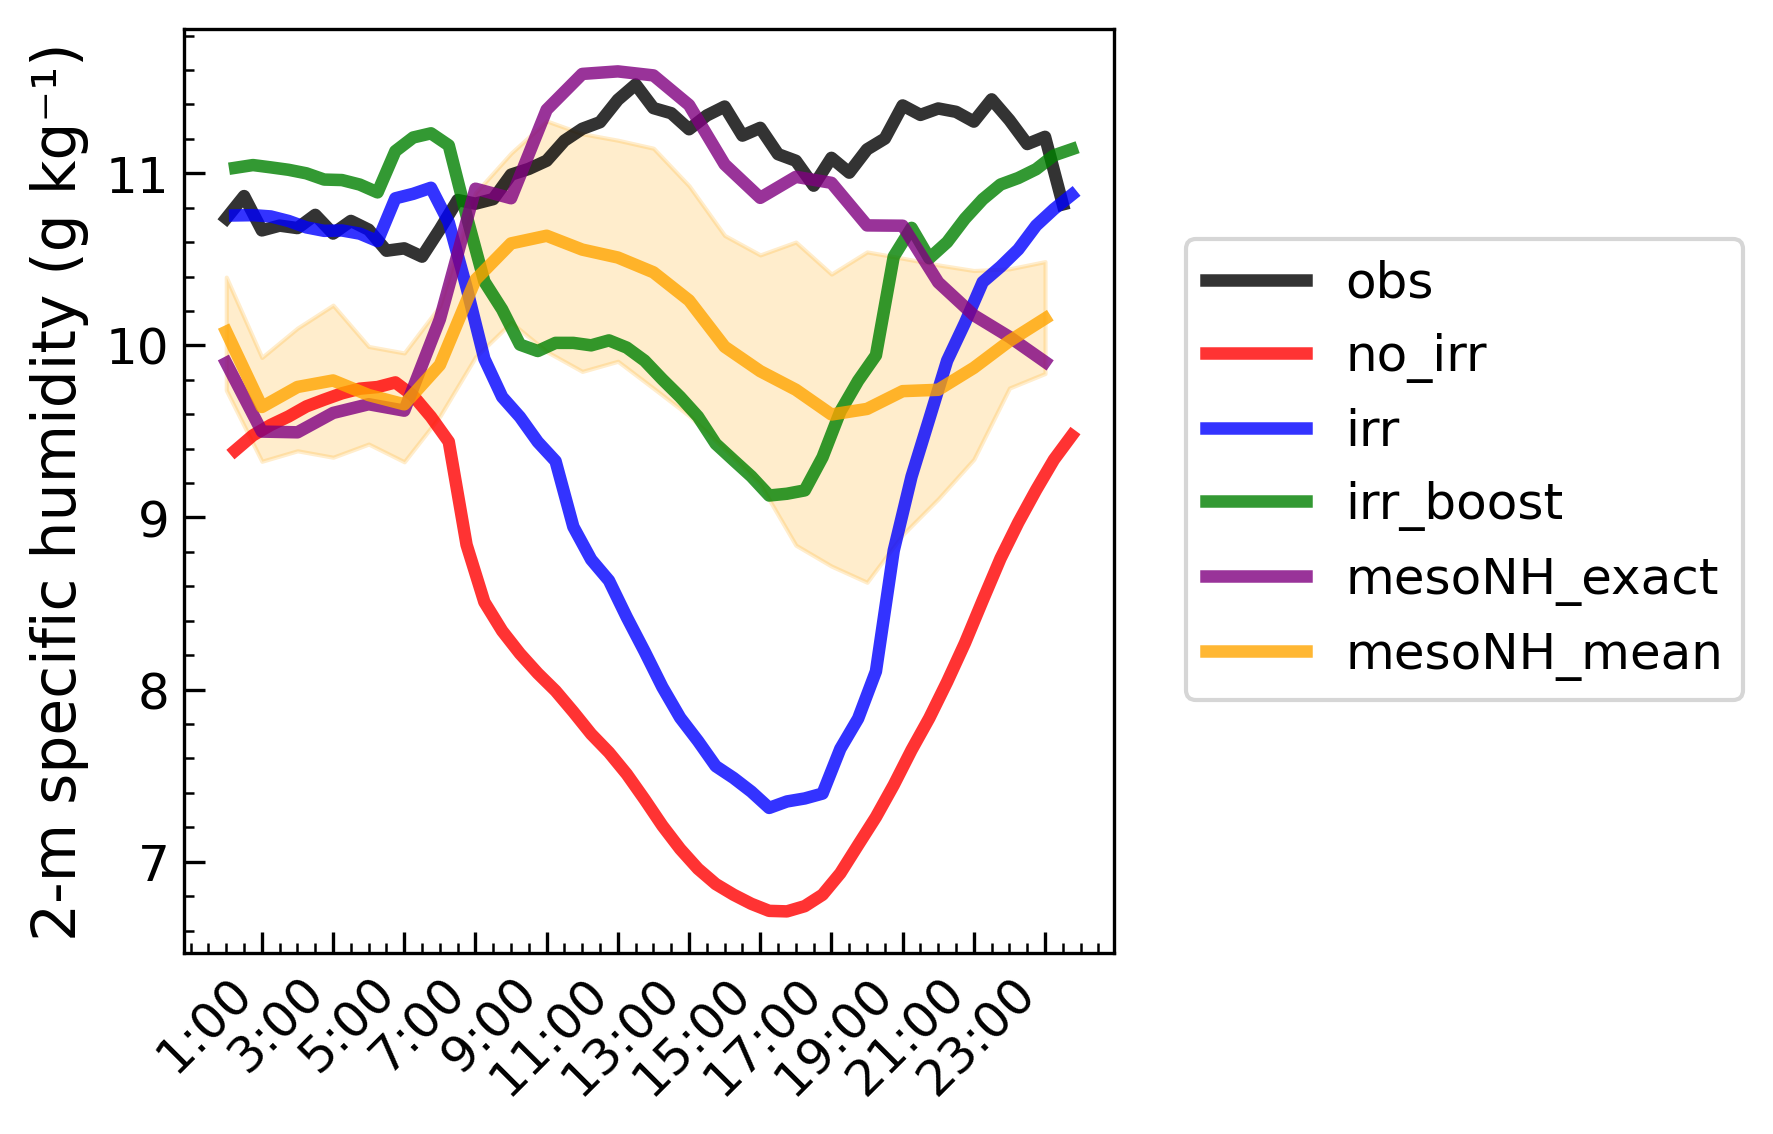
\includegraphics[width=\textwidth]{images/chap6/SOP_TS_DC/diurnal_cycle_cendrosa_q2m.png}
        \end{subfigure}
    \end{tabular}
    \caption{Time series and mean diurnal cycle (14-30 July) of surface turbulent fluxes (a-d), temperature (e-f) and specific humidity (g-h) at La Cendrosa (irrigated site). The envelope for \mesomean represents the 25th and 75th percentiles of the distribution.}
    \label{fig:cendrosa_surfacevars}
\end{figure}


%Fig : Wind on both sites
\begin{figure}[t]
    \centering
    \begin{tabular}{cc}
        \begin{subfigure}[t]{0.5\textwidth}
            \caption{10-meter wind speed (La Cendrosa)}
            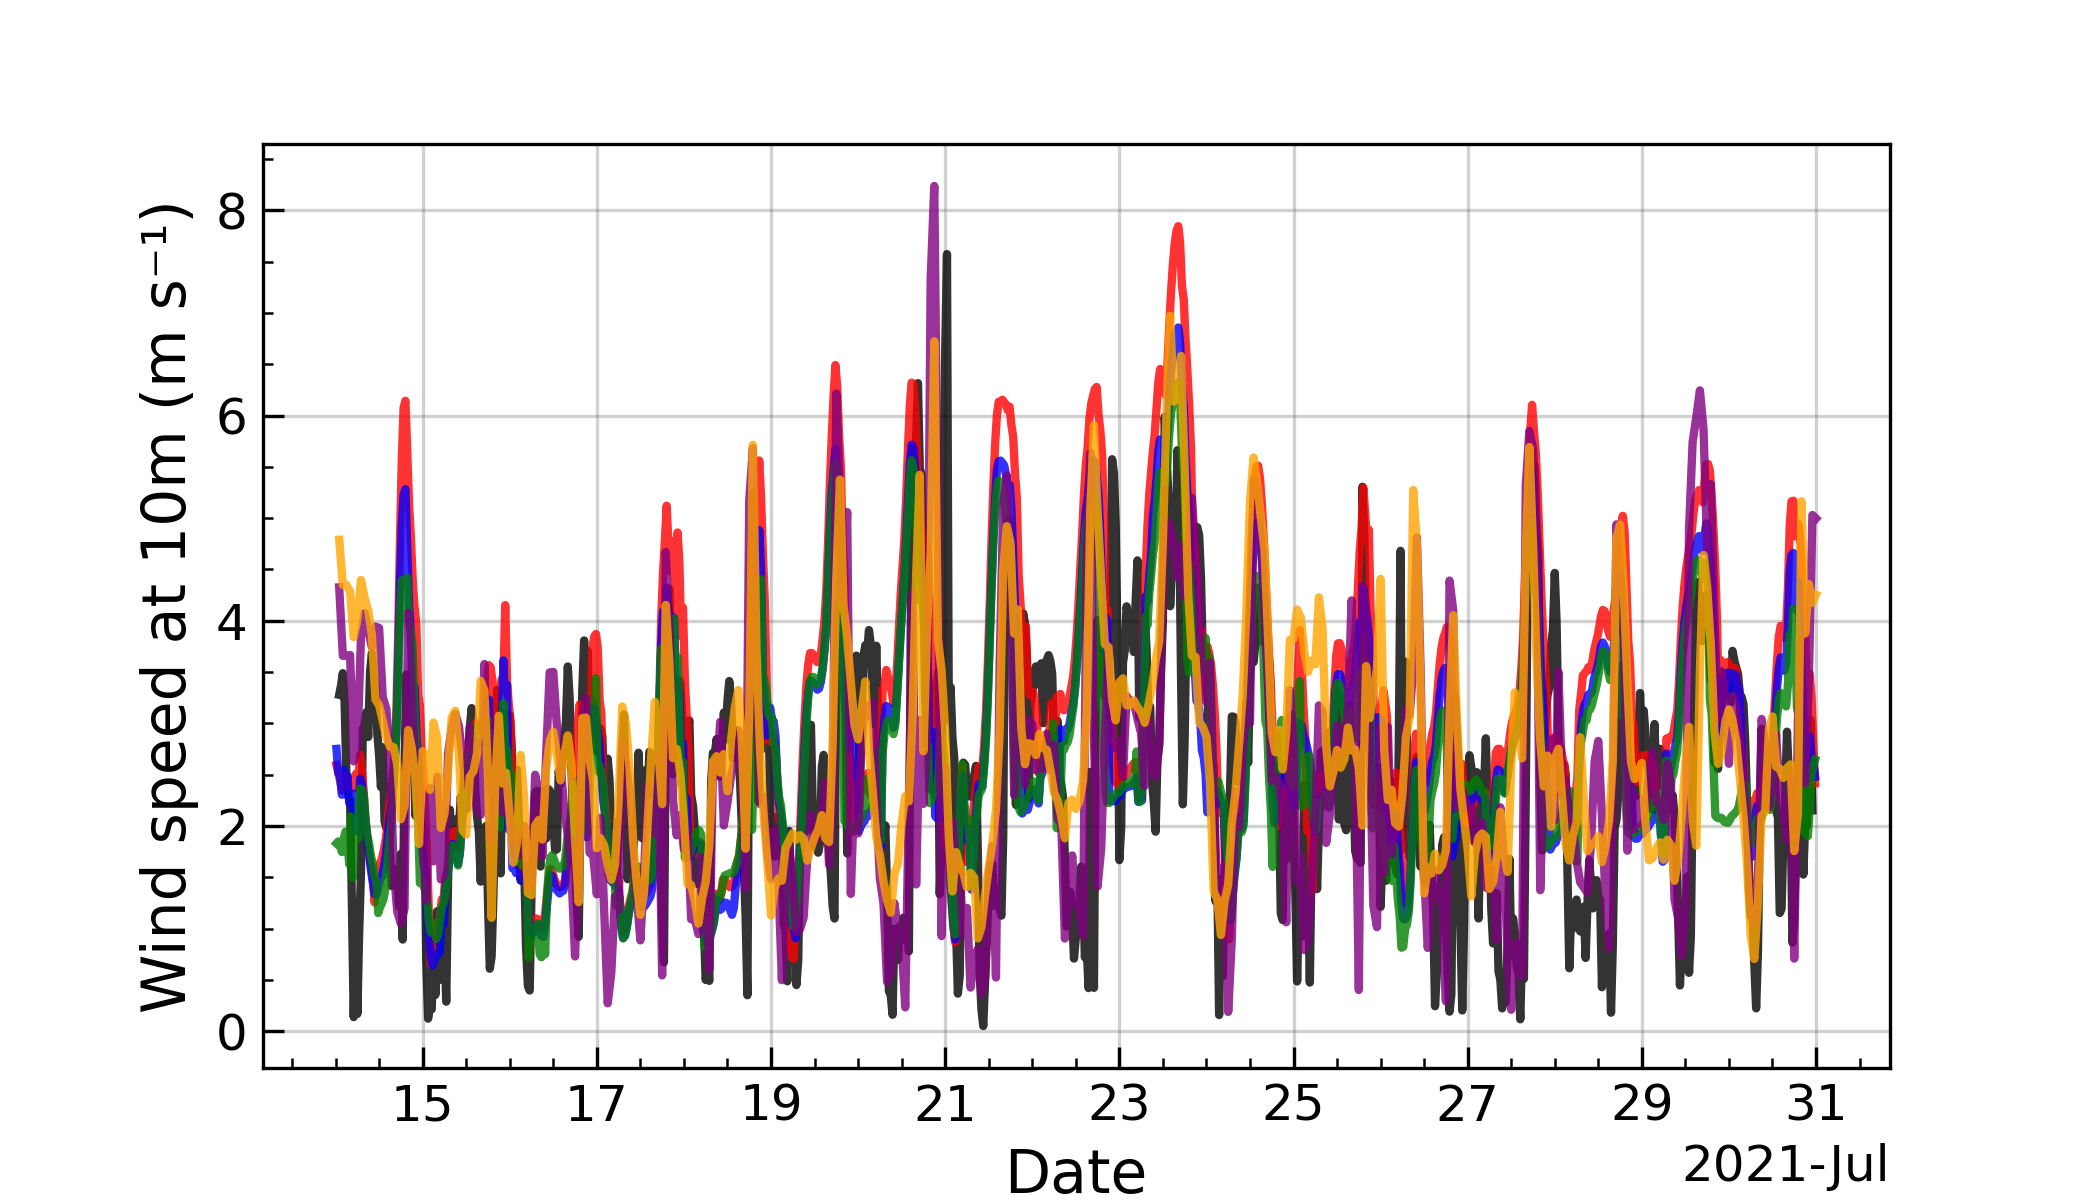
\includegraphics[width=\textwidth]{images/chap6/SOP_TS_DC/time_series_cendrosa_wind_speed_10m.png}
        \end{subfigure} &
        \begin{subfigure}[t]{0.5\textwidth}
            \caption{Mean diurnal cycle of 10-meter wind speed\\(14-30 July - La Cendrosa)}
            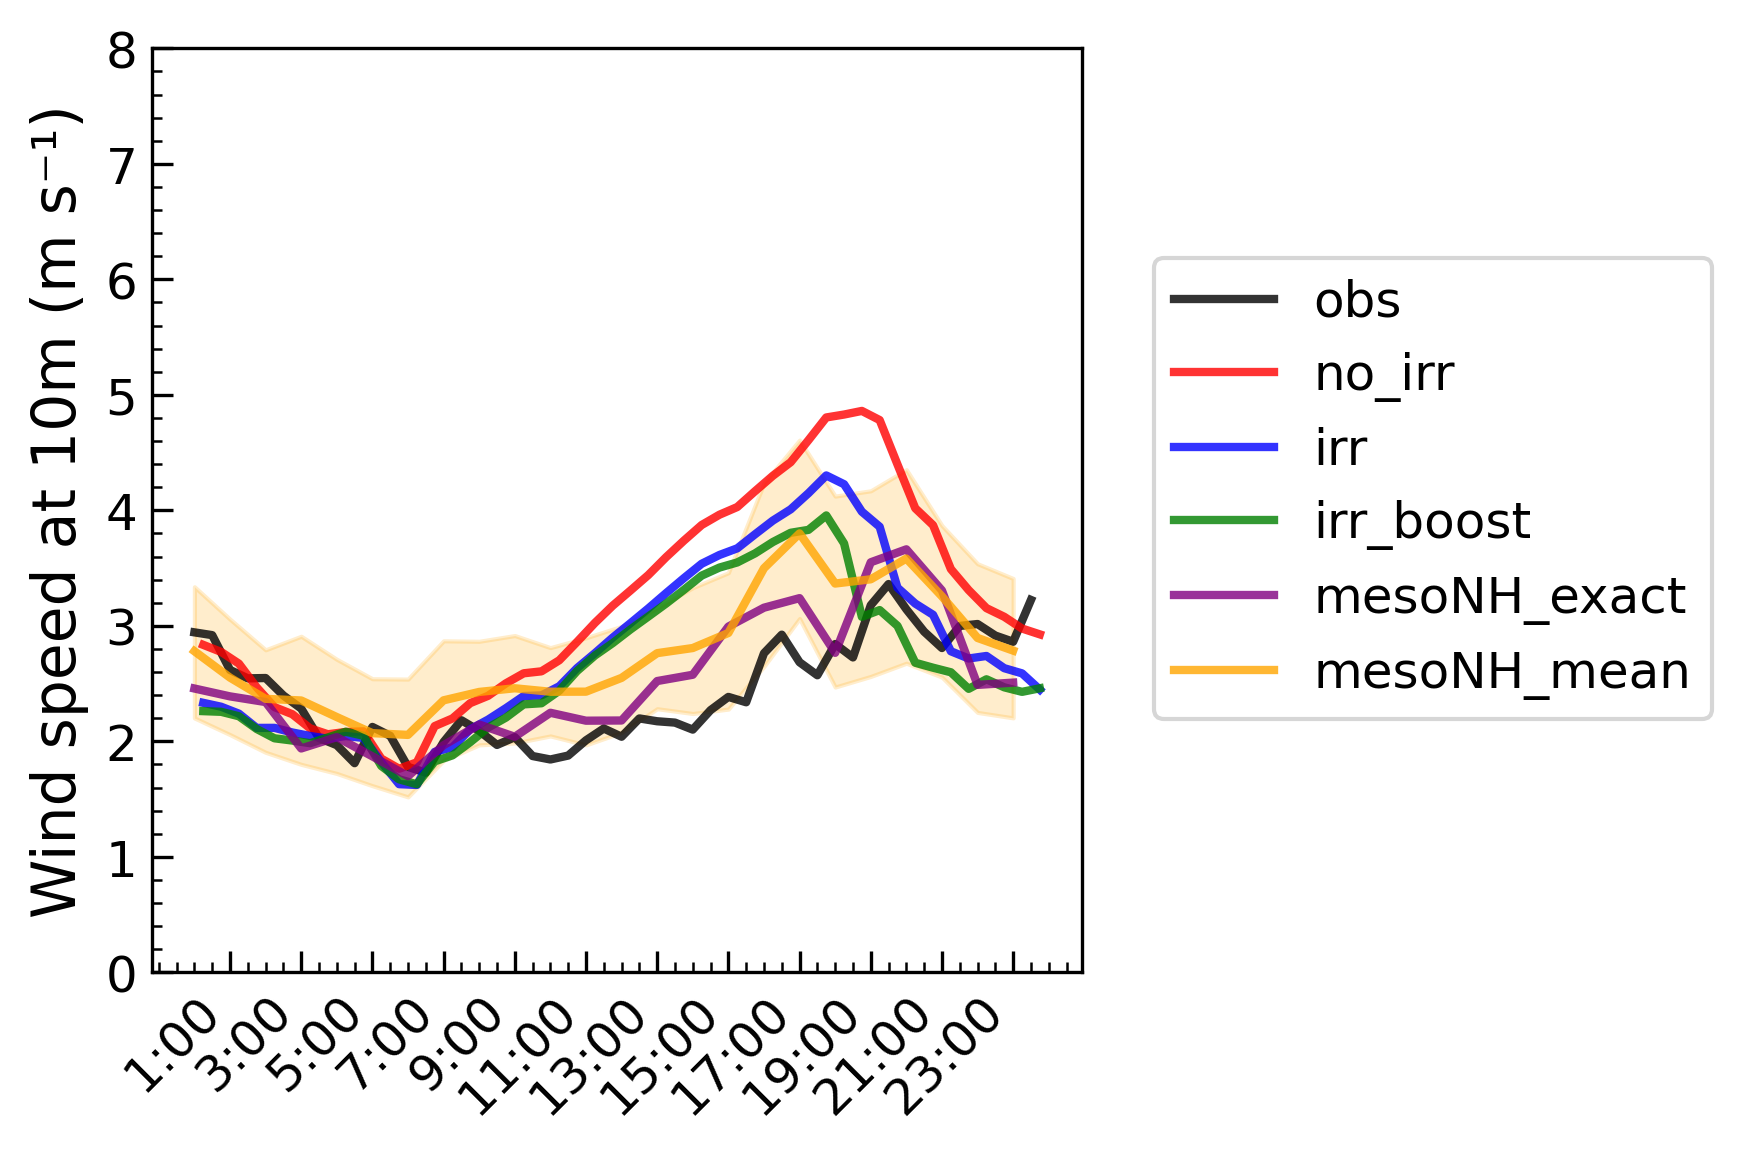
\includegraphics[width=\textwidth]{images/chap6/SOP_TS_DC/diurnal_cycle_cendrosa_wind_speed_10m.png}
        \end{subfigure} \\
        \begin{subfigure}[t]{0.5\textwidth}
            \caption{10-meter wind direction (La Cendrosa)}
            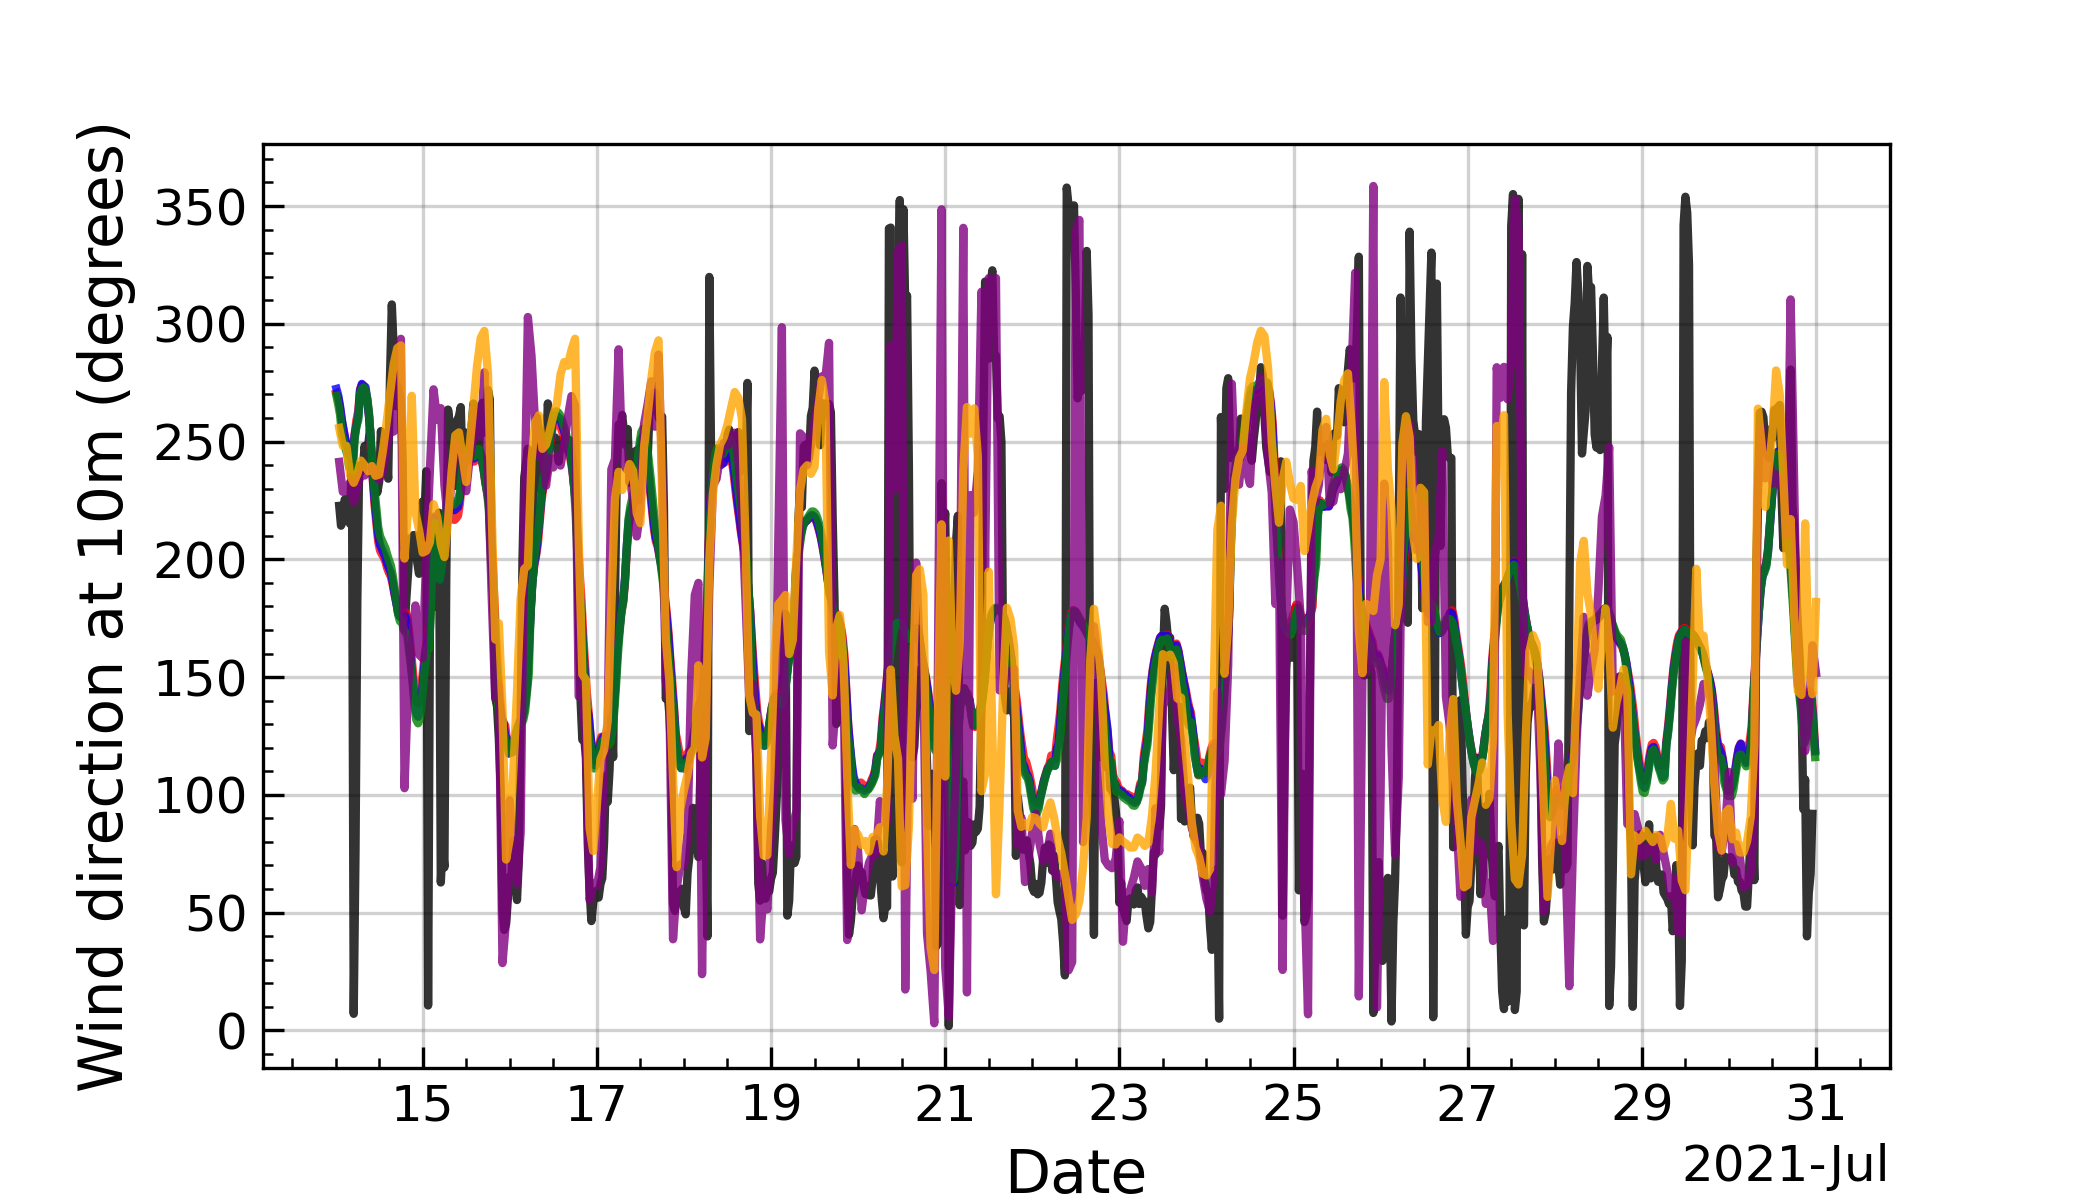
\includegraphics[width=\textwidth]{images/chap6/SOP_TS_DC/time_series_cendrosa_wind_direction_10m.png}
        \end{subfigure} &
        \begin{subfigure}[t]{0.5\textwidth}
            \caption{Mean diurnal cycle of 10-meter wind direction\\(14-30 July - La Cendrosa)}
            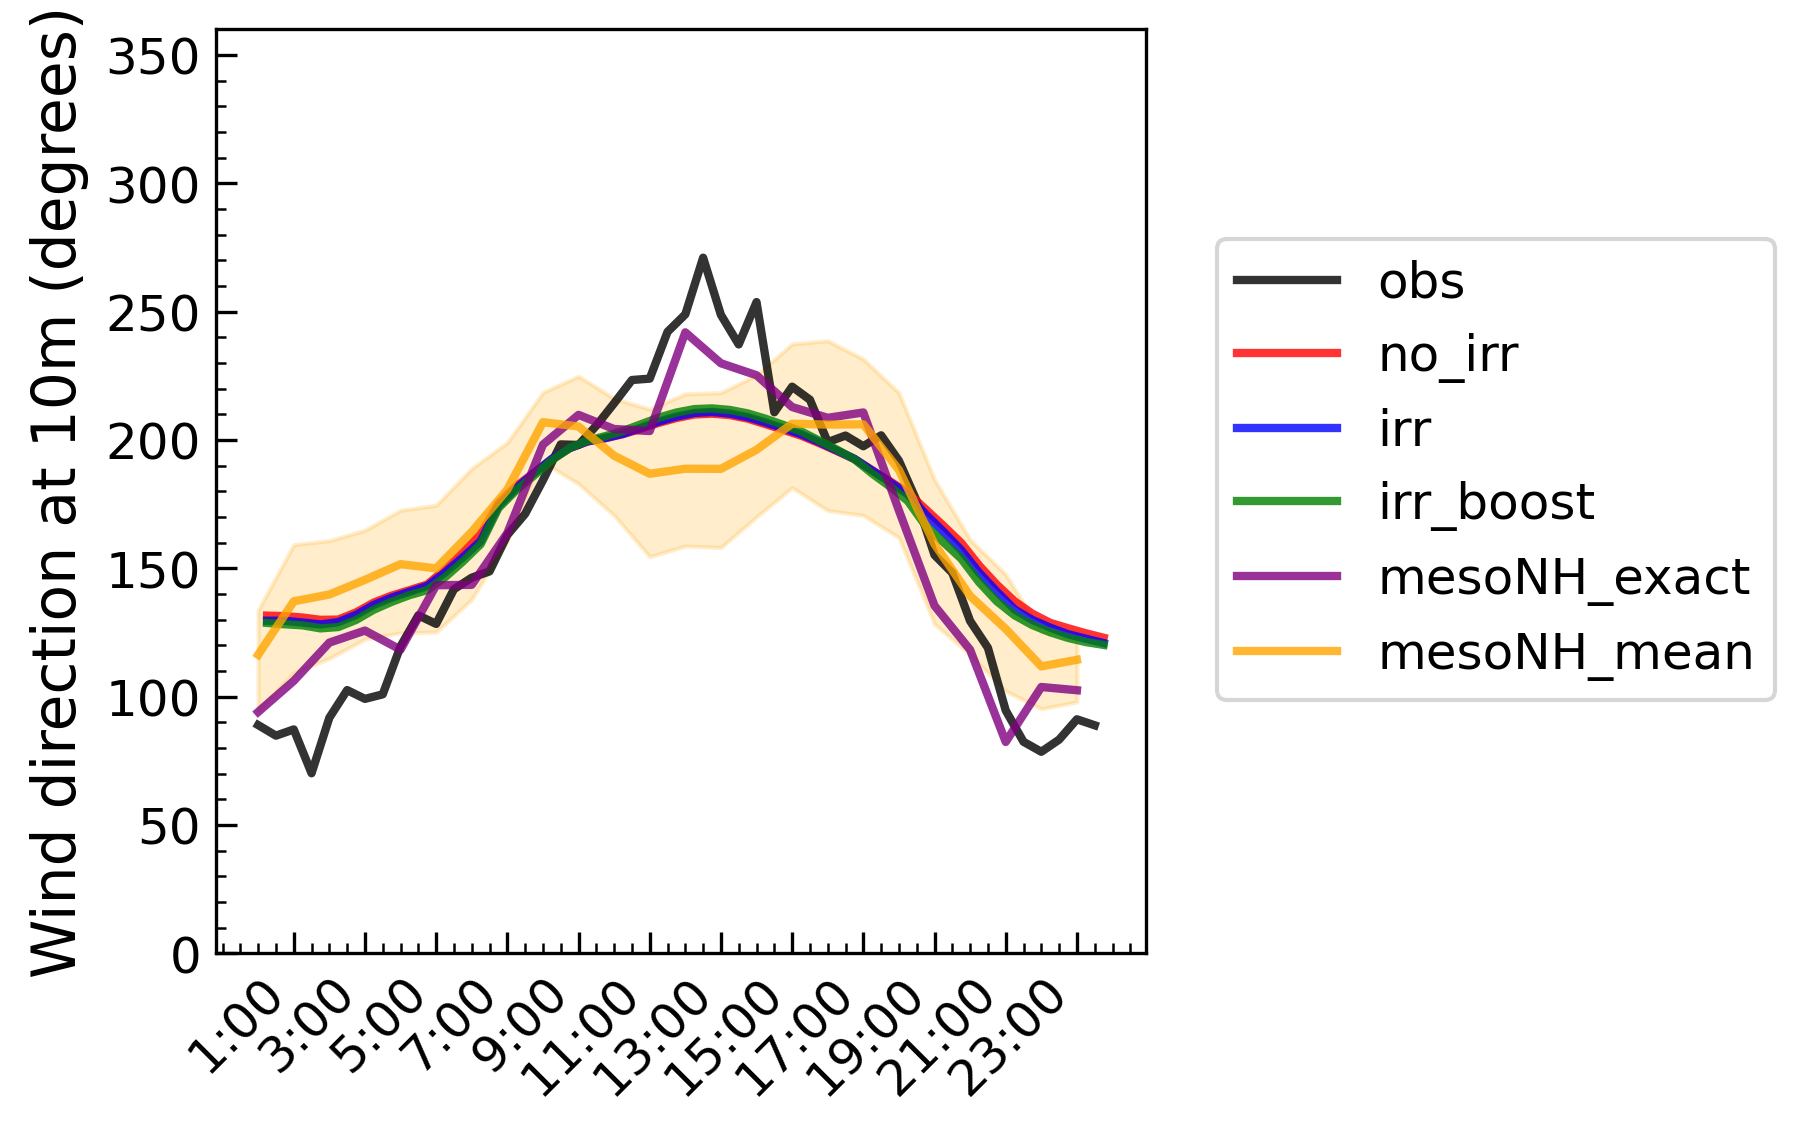
\includegraphics[width=\textwidth]{images/chap6/SOP_TS_DC/diurnal_cycle_cendrosa_wind_direction_10m.png}
        \end{subfigure} \\
        \begin{subfigure}[t]{0.5\textwidth}
            \caption{10-meter wind speed (Els Plans)}
            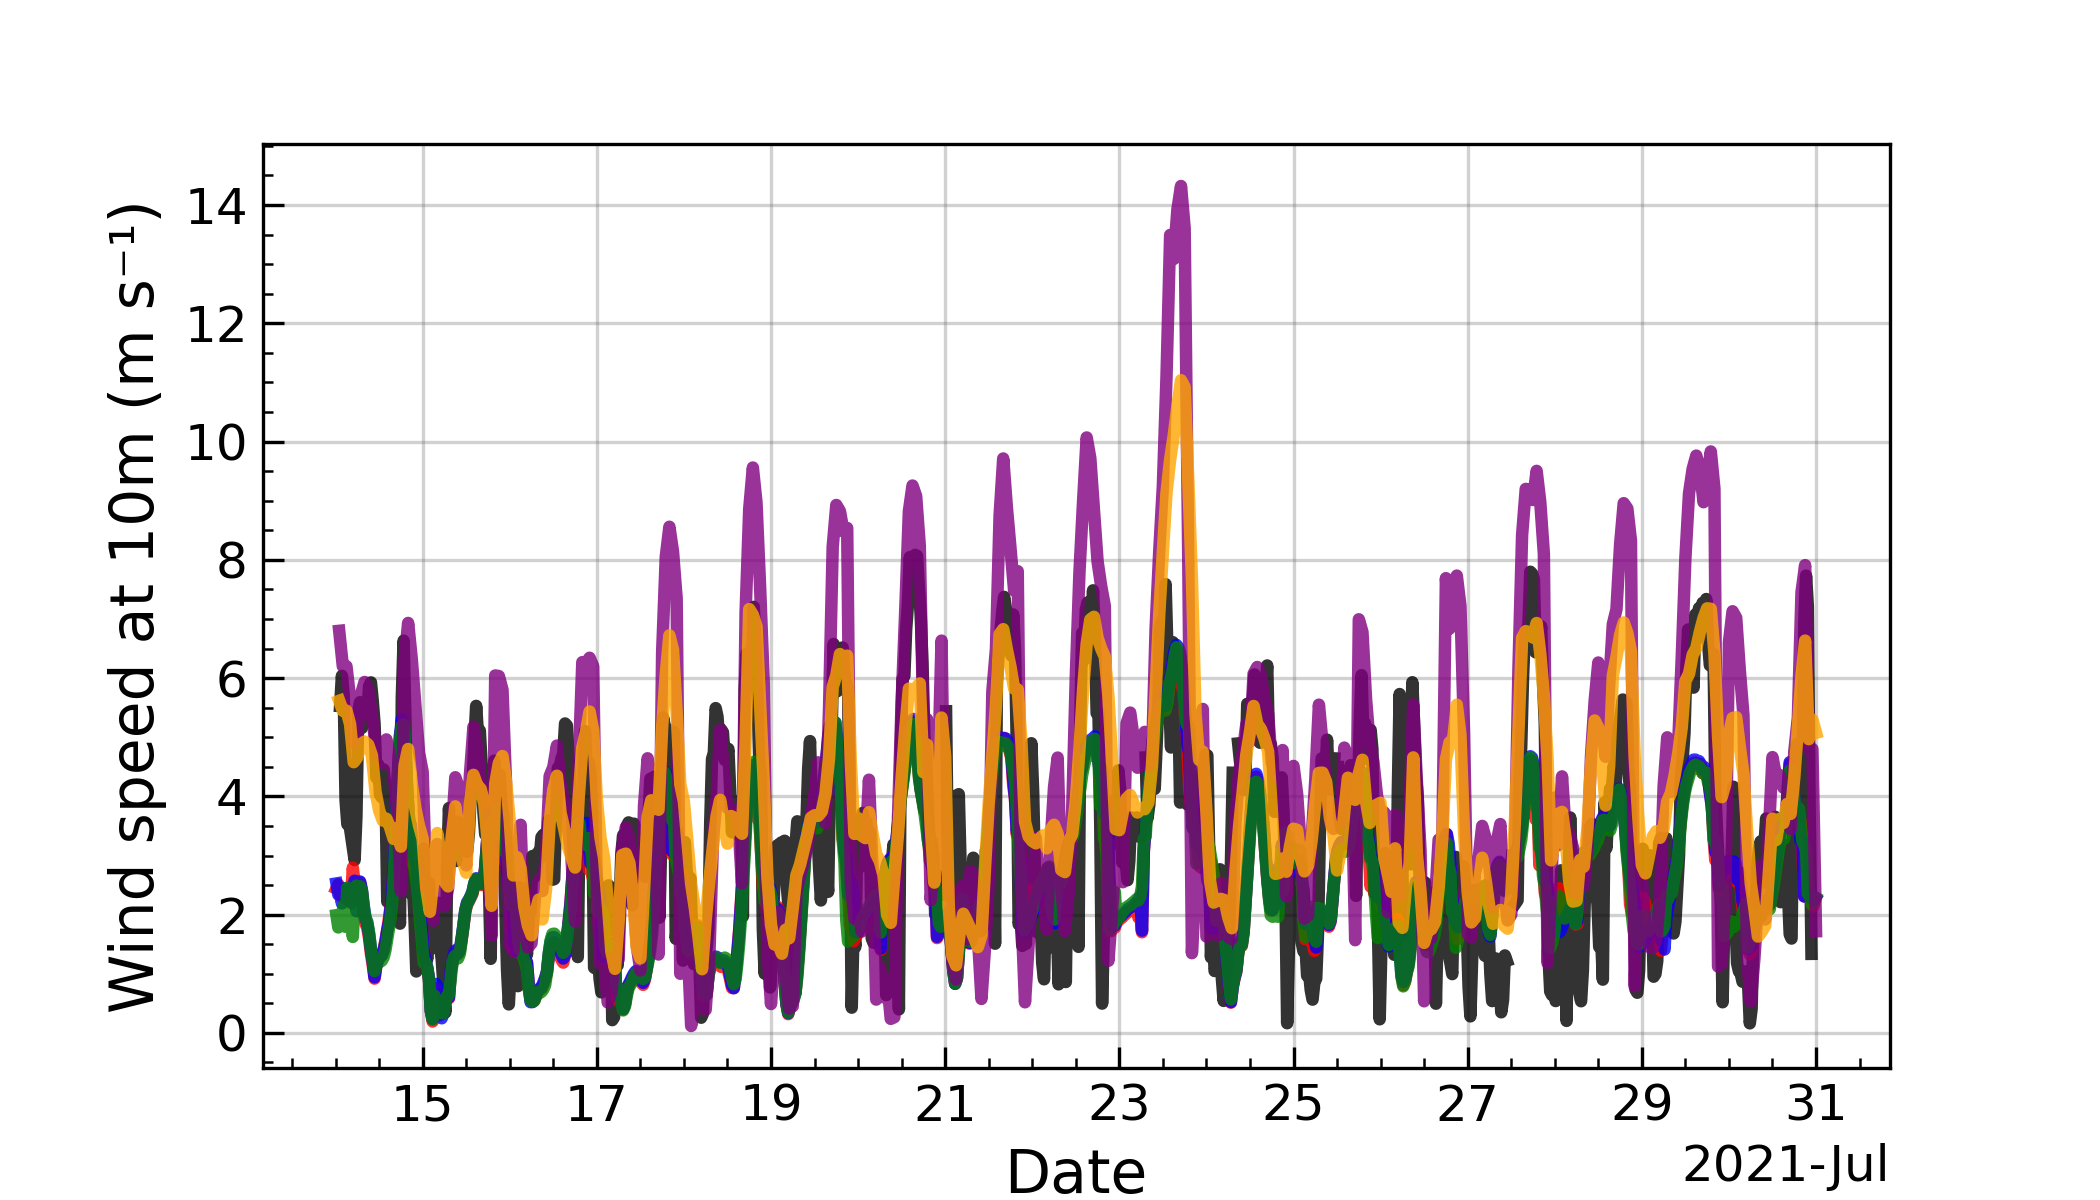
\includegraphics[width=\textwidth]{images/chap6/SOP_TS_DC/time_series_elsplans_wind_speed_10m.png}
        \end{subfigure} &
        \begin{subfigure}[t]{0.5\textwidth}
            \caption{Mean diurnal cycle of 10-meter wind speed\\(14-30 July - Els Plans)}
            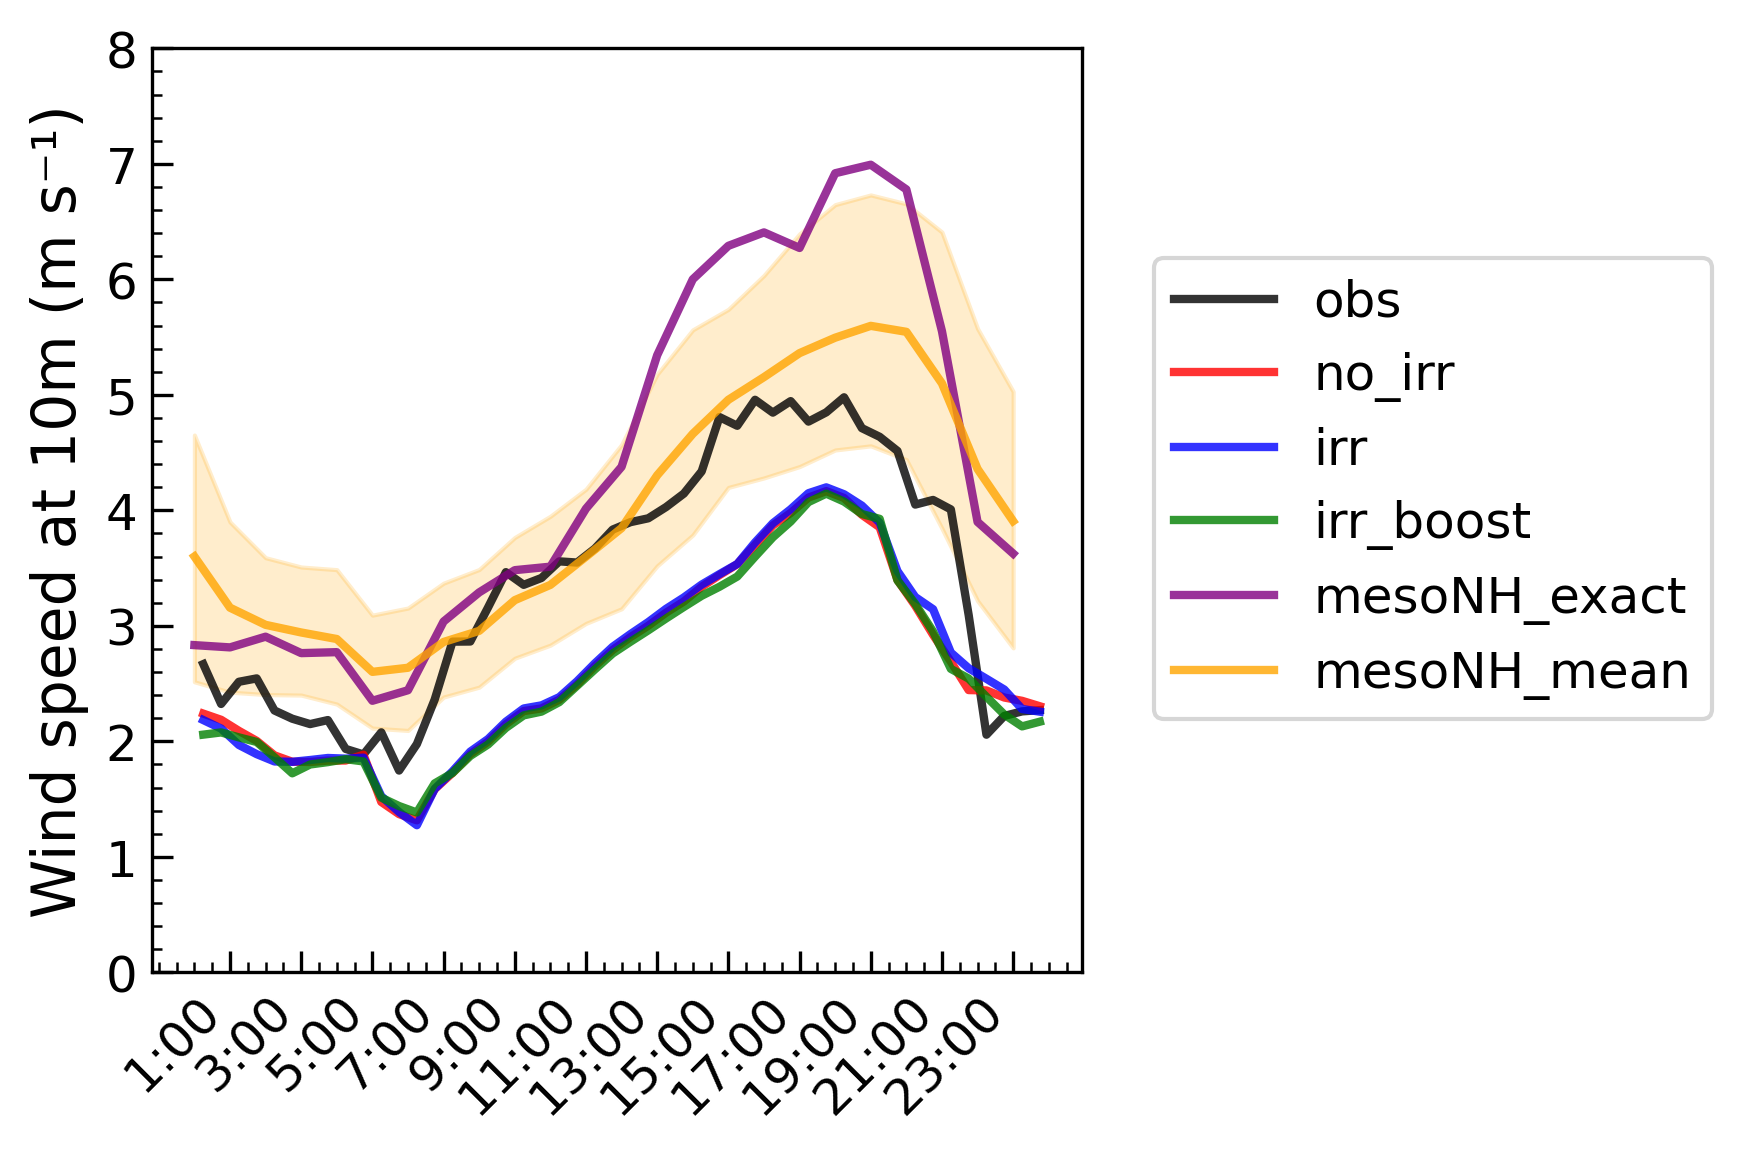
\includegraphics[width=\textwidth]{images/chap6/SOP_TS_DC/diurnal_cycle_elsplans_wind_speed_10m.png}
        \end{subfigure} \\
        \begin{subfigure}[t]{0.5\textwidth}
            \caption{10-meter wind direction (Els Plans)}
            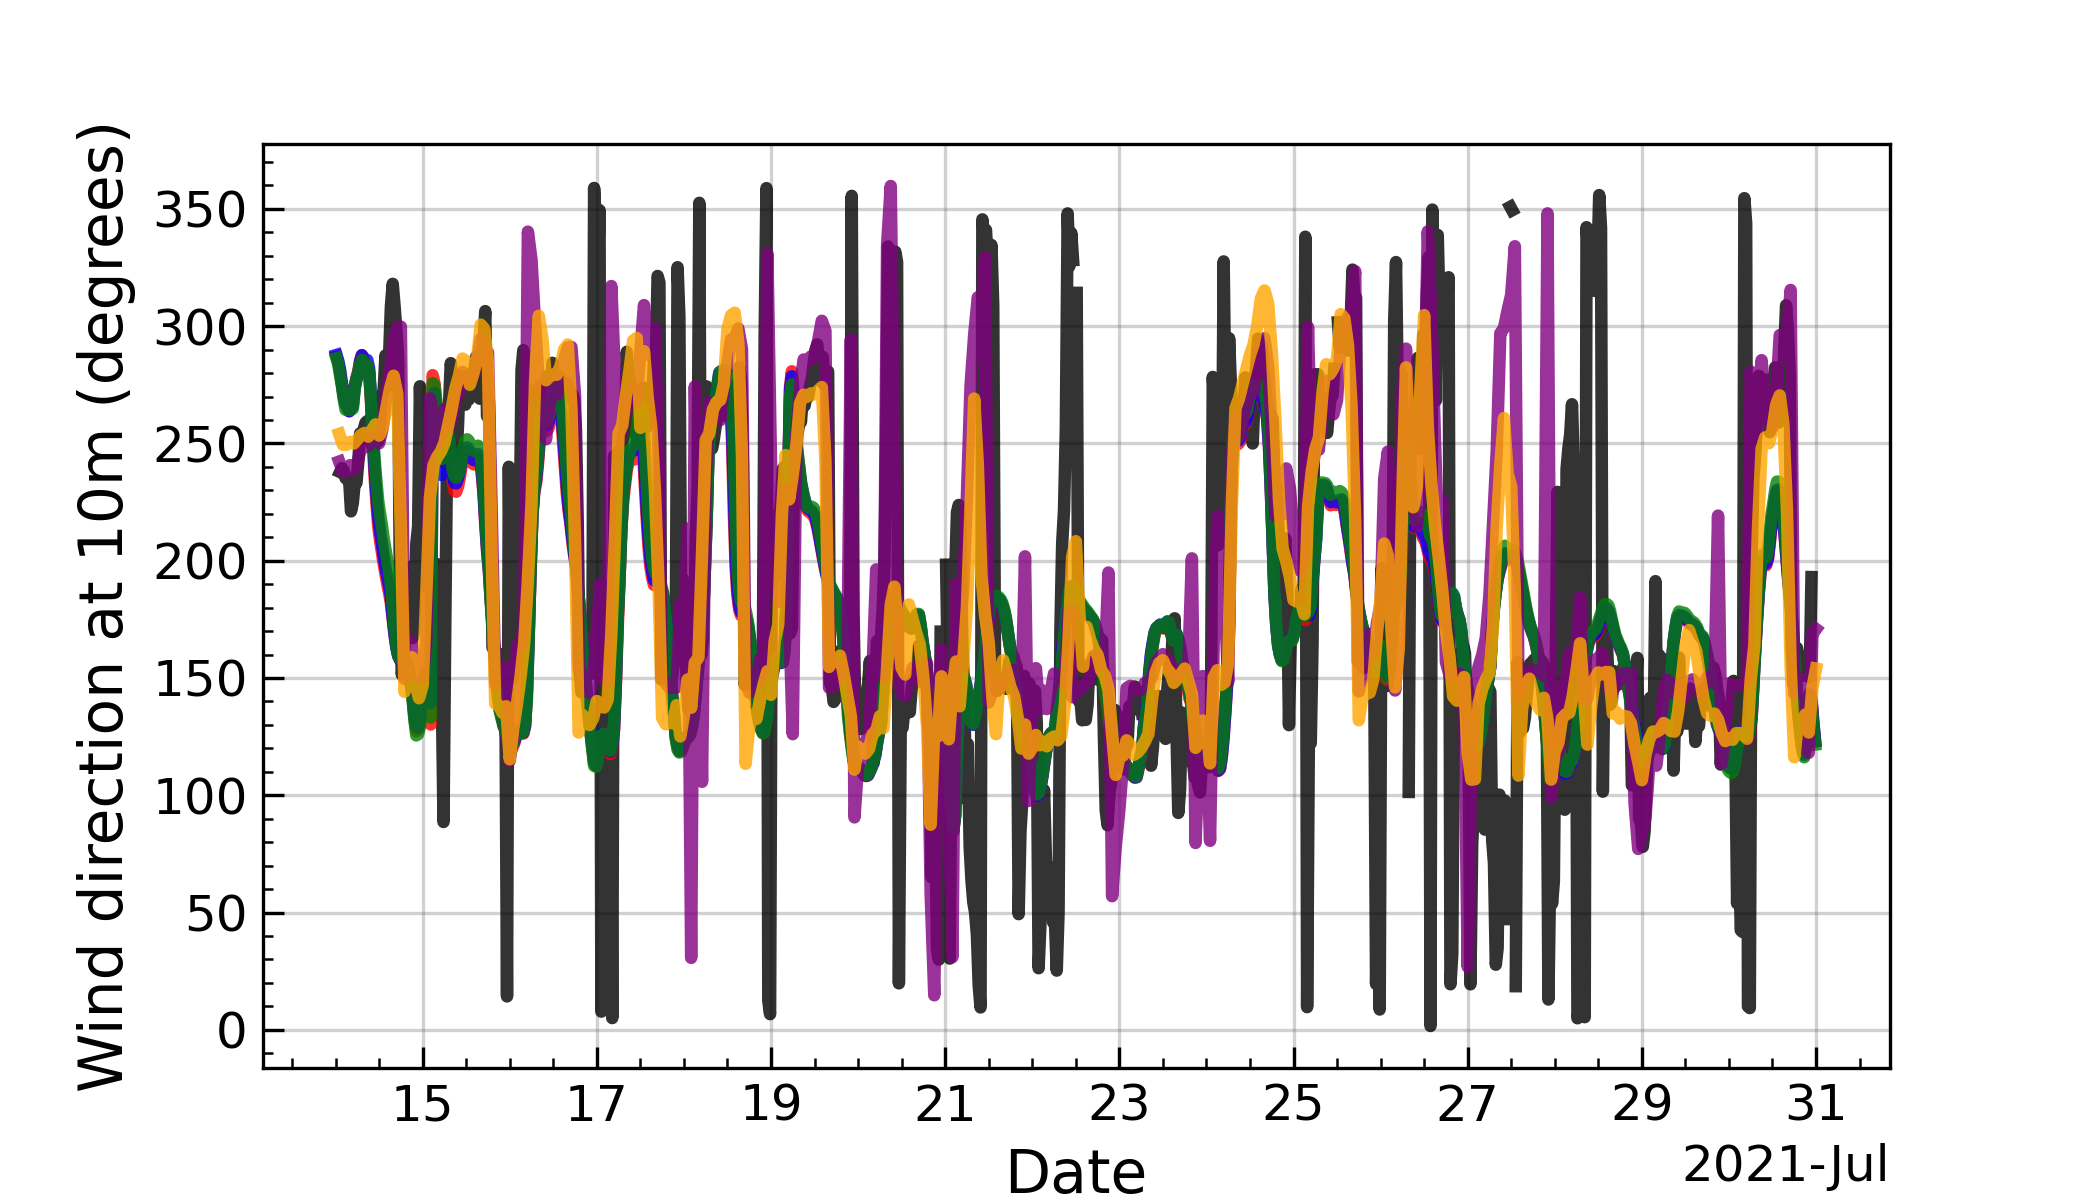
\includegraphics[width=\textwidth]{images/chap6/SOP_TS_DC/time_series_elsplans_wind_direction_10m.png}
        \end{subfigure} &
        \begin{subfigure}[t]{0.5\textwidth}
            \caption{Mean diurnal cycle of 10-meter wind direction\\(14-30 July - Els Plans)}
            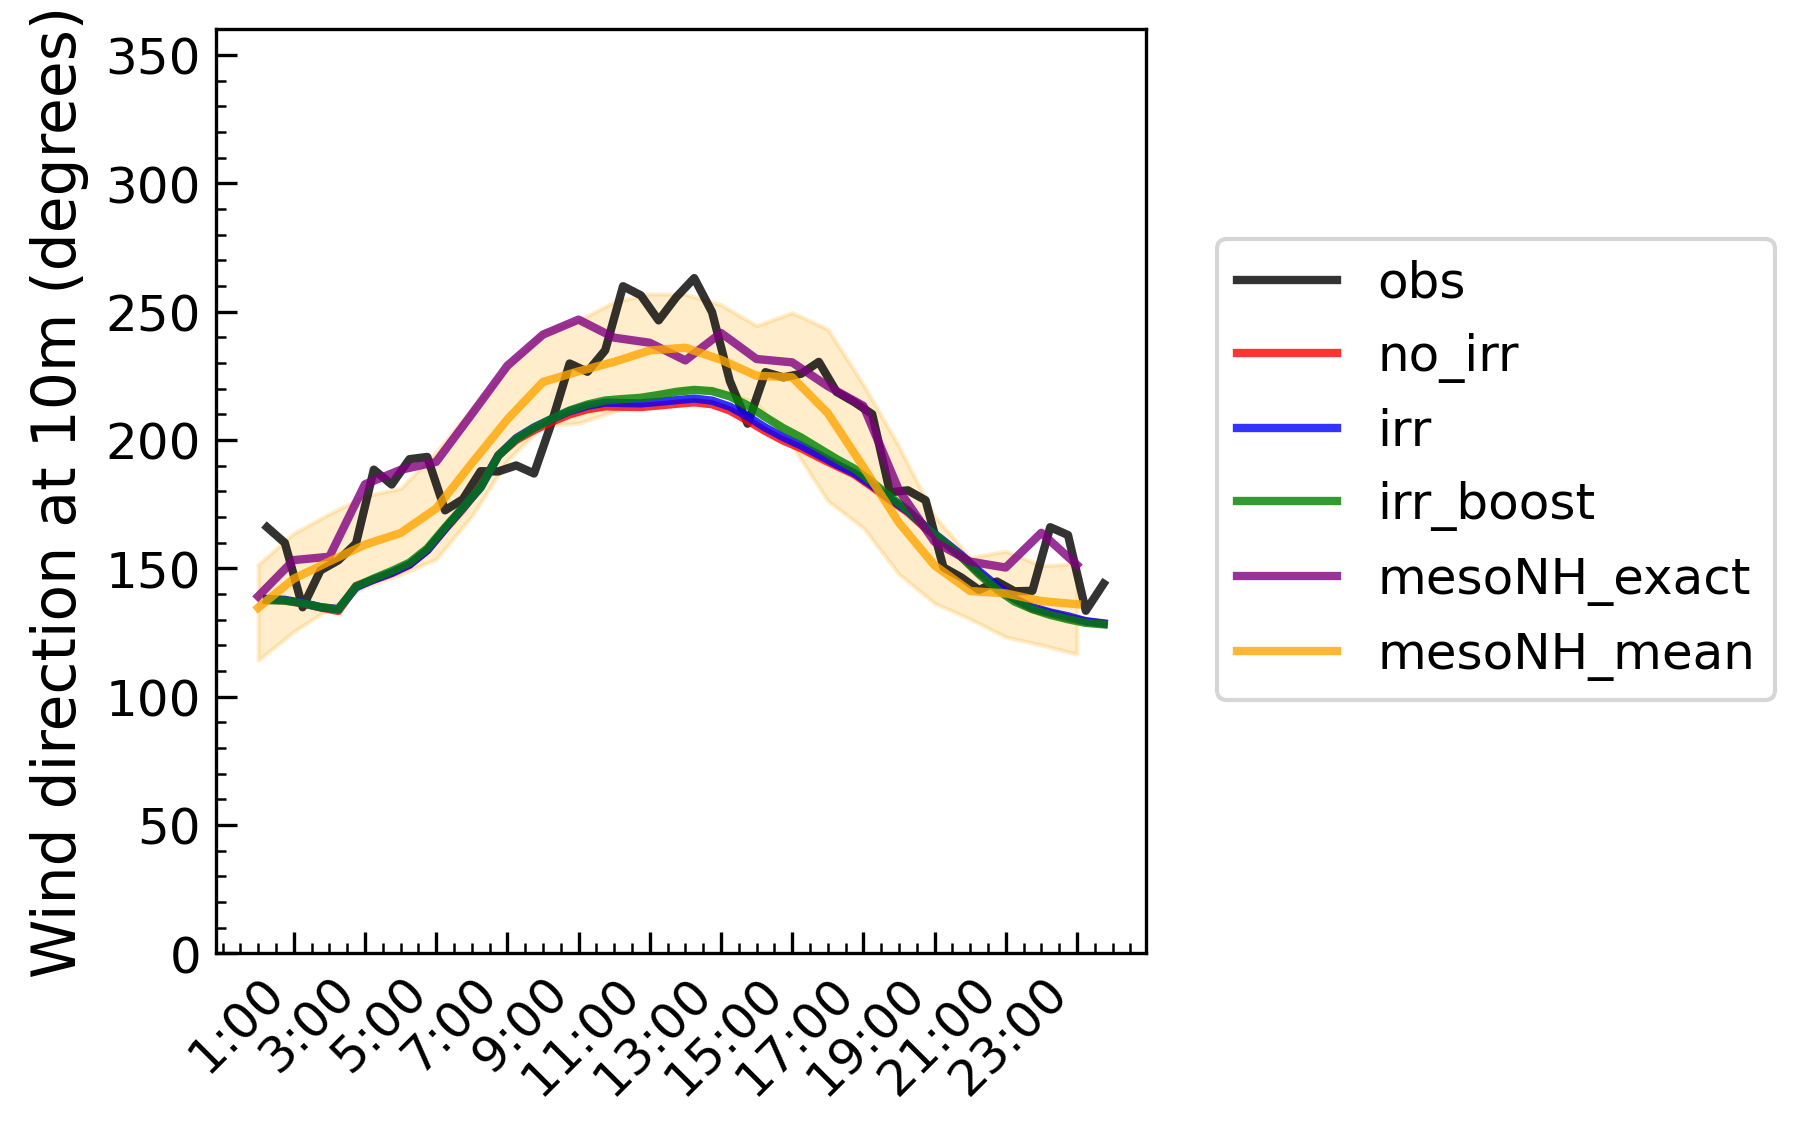
\includegraphics[width=\textwidth]{images/chap6/SOP_TS_DC/diurnal_cycle_elsplans_wind_direction_10m.png}
        \end{subfigure}
    \end{tabular}
    \caption{Time series and mean diurnal cycle of 10-meter wind speed and direction on both sites, 14-30 July 2021. The envelope for \mesomean represents the 25th and 75th percentiles of the distribution.}
    \label{fig:bothsites_wind}
\end{figure}

\clearpage

\subsubsection*{Els Plans}
Looking into near-surface conditions at the Els Plans site (Fig. \ref{fig:elsplans_surfacevars}) serves as a useful comparison to assess the general performance of both models in a context that is much more independent of soil moisture.
The energy partitioning between turbulent fluxes is very different, since the average observed latent heat flux is below 20 W \persqm while the sensible heat flux is three times larger than at La Cendrosa (Fig. \ref{fig:elsplans_surfacevars}b, d). 
The three ICOLMDZ simulations are very similar and the lines for \noirr and \irr completely overlap, while latent heat flux is slightly increased (5-10 W \persqm) in \irrboost because ORCHIDEE still computes a small irrigation for this grid cell. This is due to the back-and-forth interpolation between the hexagonal ORCHIDEE grid (where irrigation demand is computed, and water is eventually infiltrated) and the regular routing grid (where irrigation is computed), which can lead to small irrigation volumes even if the initial demand is zero.
ICOLMDZOR underestimates the already weak latent heat flux and overestimates the sensible heat flux with a peak value higher than 400 W \persqm whereas the observed one is around 300 W \persqm. 
Regarding the Meso-NH simulation, the \mesoexact diurnal cycle of latent heat flux looks a bit different from the observed one, with a higher and sharper peak around 12UTC instead of the smooth shape seen in observations. The diurnal cycle of sensible heat flux matches the observed shape but presents an overestimation from 11UTC until the evening.
The latent heat flux of \mesomean is clearly driven by the few irrigated grid cells that fall into the hexagon (Fig. \ref{fig:liaise_sites_grid_cells}c), leading the mean value to exceed the 75th percentile. These outliers have much less influence on the sensible heat flux which shows a smaller spread and is even closer to observations than \mesoexact.
On the contrary to La Cendrosa, it was not really expected to see the \irr or \irrboost simulation matching \mesomean because the input map of irrigated fraction was voluntarily modified to limit irrigation on this grid cell. This was done with the initial objectives of creating a constrated situation compared to La Cendrosa and achieving a better match with on-site observations, but clearly made the comparison of grid-cell average fluxes less relevant.
%option:add that no big reservoir here so no irrigation at all if not cheating ? (and too much if cheating ?)

The average diurnal cycle of 2-meter temperature (Fig. \ref{fig:elsplans_surfacevars}f) confirms the presence of a warm bias in Meso-NH at night (more than 2°C), and shows a slight underestimation of the peak value in the afternoon. 
%option: further links to fsens, LWup, Tsurf ?
%NB : sur les deux sites, LWdn est sous estimé de ~15W/m² en journée par les deux modèles (sauf \noirr sur La Cendrosa car air plus chaud), probablement ce qui permet d'être bon sur fsens alors que flat est surestimé (manque d'énergie incidente donc pas de compensation parfaite entre les deux)
It also highlights the very good performance of ICOLMDZOR on this non-irrigated site, although the peak is slightly too early compared to the observed one, as also seen at La Cendrosa.

The observed evolution of 2-meter specific humidity over the day is very different from La Cendrosa, since it is highest at night and steadliy decreases throughout the day with a minimal peak at 16UTC on average over the SOP (Fig. \ref{fig:elsplans_surfacevars}h).
As seen in La Cendrosa, Meso-NH exhibits a dry bias at night but simulates correct humidity in the day. 
The diurnal evolution simulated by ICOLMDZOR is quite similar to the one at La Cendrosa, except that at Els Plans it is more in agreement with observations and Meso-NH. On average over the SOP, ICOLMDZOR strongly underestimates 2-meter specific humidity, but as visible in Fig. \ref{fig:elsplans_surfacevars}g, this is mostly due to the second part of the SOP where excessive drying occurs in all three ICOLMDZOR simulations. 
This supports the idea that the limitations in capturing near-surface humidity variations at La Cendrosa are mostly non-local and induced by large-scale advection. 
Finally, it can be noticed that irrigation in has a visible impact on specific humidity, although not very large in comparison to the dry bias.
This might be due to the small irrigation volumes computed for this grid cell but considering how small they are (especially in \irr) it also points to non-local effects through the advection of moisture from neighbouring irrigated grid cells.

Observed wind speed at Els Plans is higher than at La Cendrosa (Fig. \ref{fig:bothsites_wind}f), which relflects the influence of roughness on a site with lower vegetation (Fig. \ref{fig:liaise_sites_photos}). On average, variations in direction are of smaller amplitude than at La Cendrosa (Fig. \ref{fig:bothsites_wind}h) but some quick regime changes can still be identified on most days (Fig. \ref{fig:bothsites_wind}g).
In ICOLMDZOR, the simulated wind speed and direction are very similar at Els Plans and La Cendrosa, which is not surprising since the grid cells are next to each other, but there are no more dfferences between the three simulations. This confirms the hypothesis that the wind speed differences at La Cendrosa were mainly the consequence of increased roughness (via LAI) in \irrboost and \irr. On average, ICOLMDZOR underestimates wind speed but reproduces the diurnal changes in wind direction. As seen at La Cendrosa, it captures the variations in wind direction much better in the beginning of the SOP than after the regime change on 20 July. On this second part of the SOP, a lot of regime changes are not represented by ICOLMDZOR and \mesomean, while only some of them are simulated in \mesoexact.

%Fig : Els Plans turbulent fluxes + t2m, q2m
\begin{figure}[hbtp]
    \centering
    \begin{tabular}{cc}
        \begin{subfigure}[t]{0.5\textwidth}
            \caption{Latent heat flux (Els Plans)}
            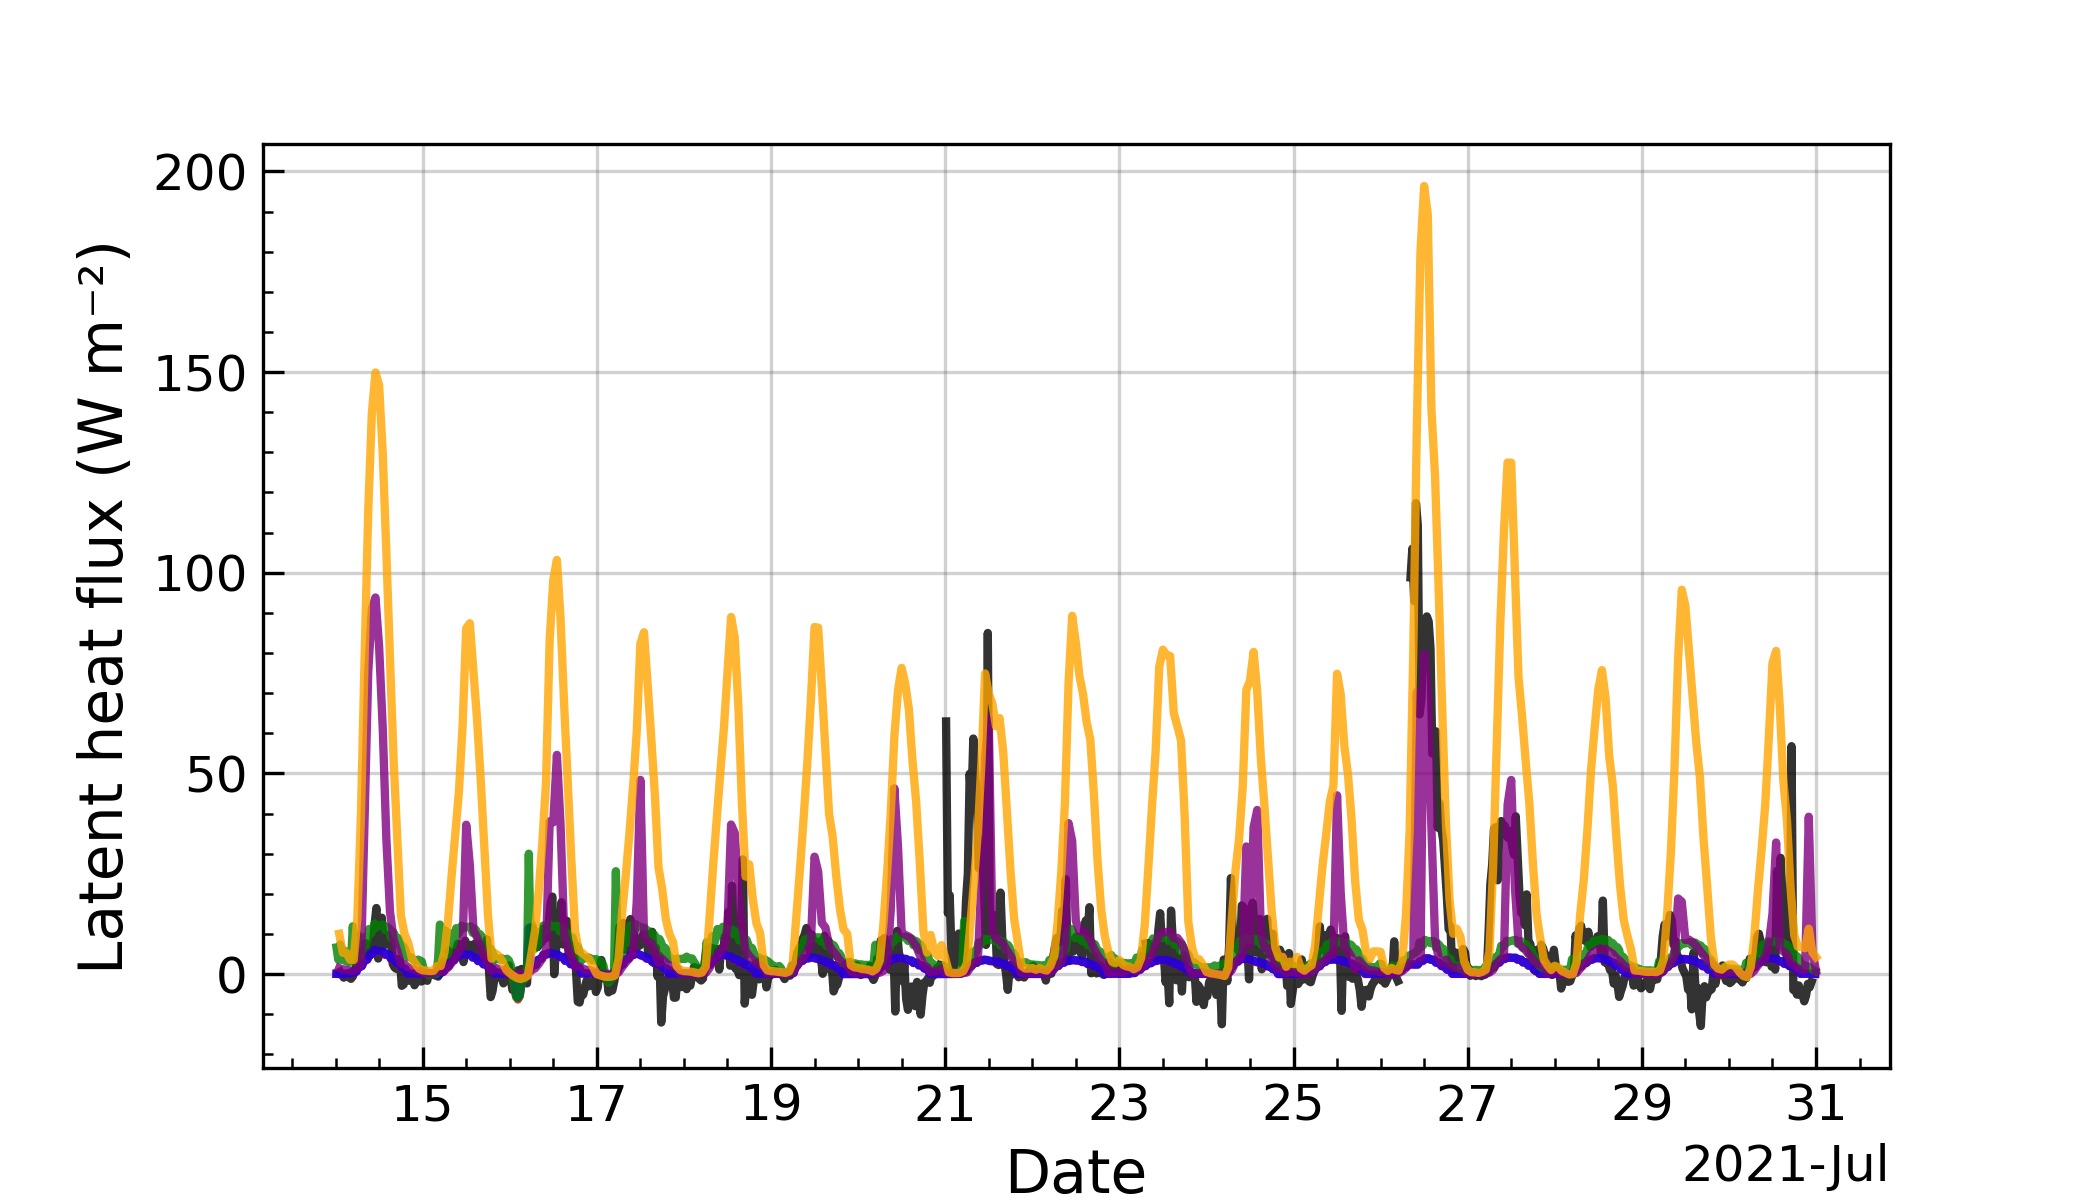
\includegraphics[width=\textwidth]{images/chap6/SOP_TS_DC/time_series_elsplans_flat.png}
        \end{subfigure} &
        \begin{subfigure}[t]{0.5\textwidth}
            \caption{Mean diurnal cycle of latent heat flux\\(14-30 July - Els Plans)}
            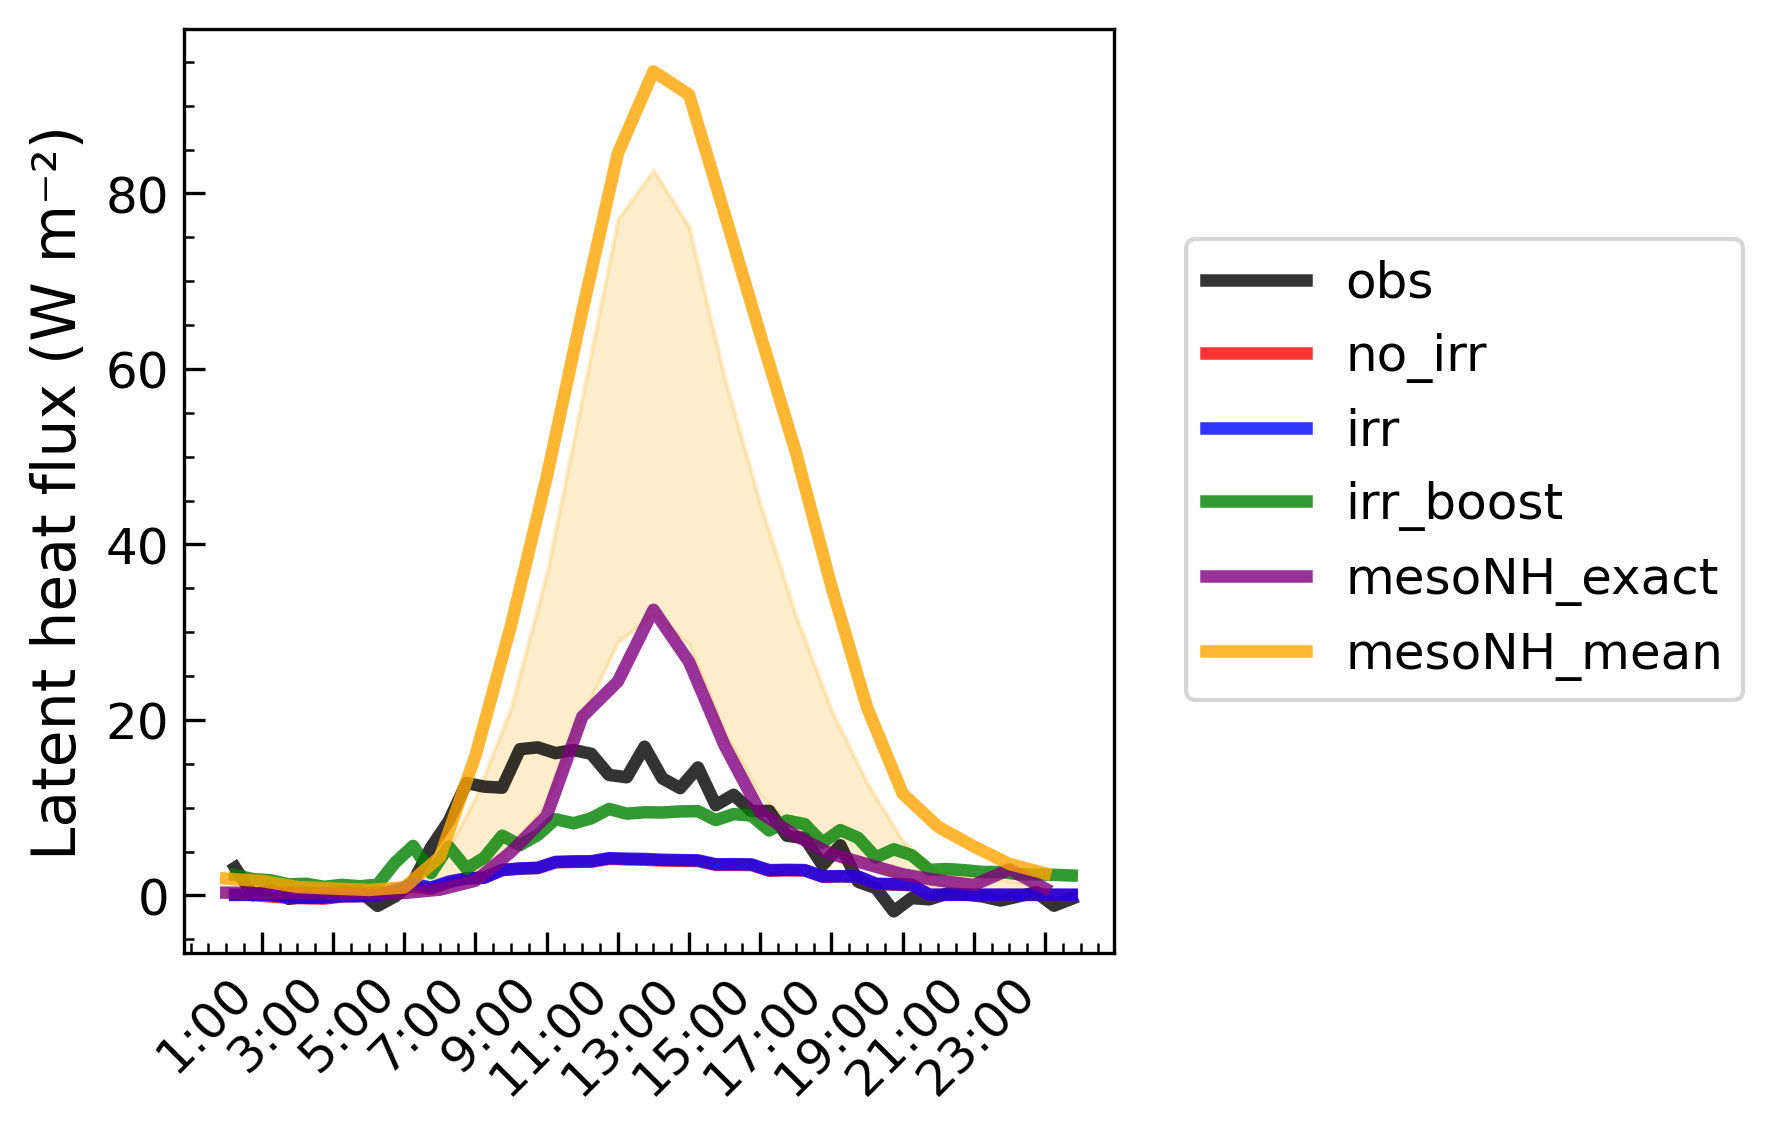
\includegraphics[width=\textwidth]{images/chap6/SOP_TS_DC/diurnal_cycle_elsplans_flat.png}
        \end{subfigure} \\
        \begin{subfigure}[t]{0.5\textwidth}
            \caption{Sensible heat flux (Els Plans)}
            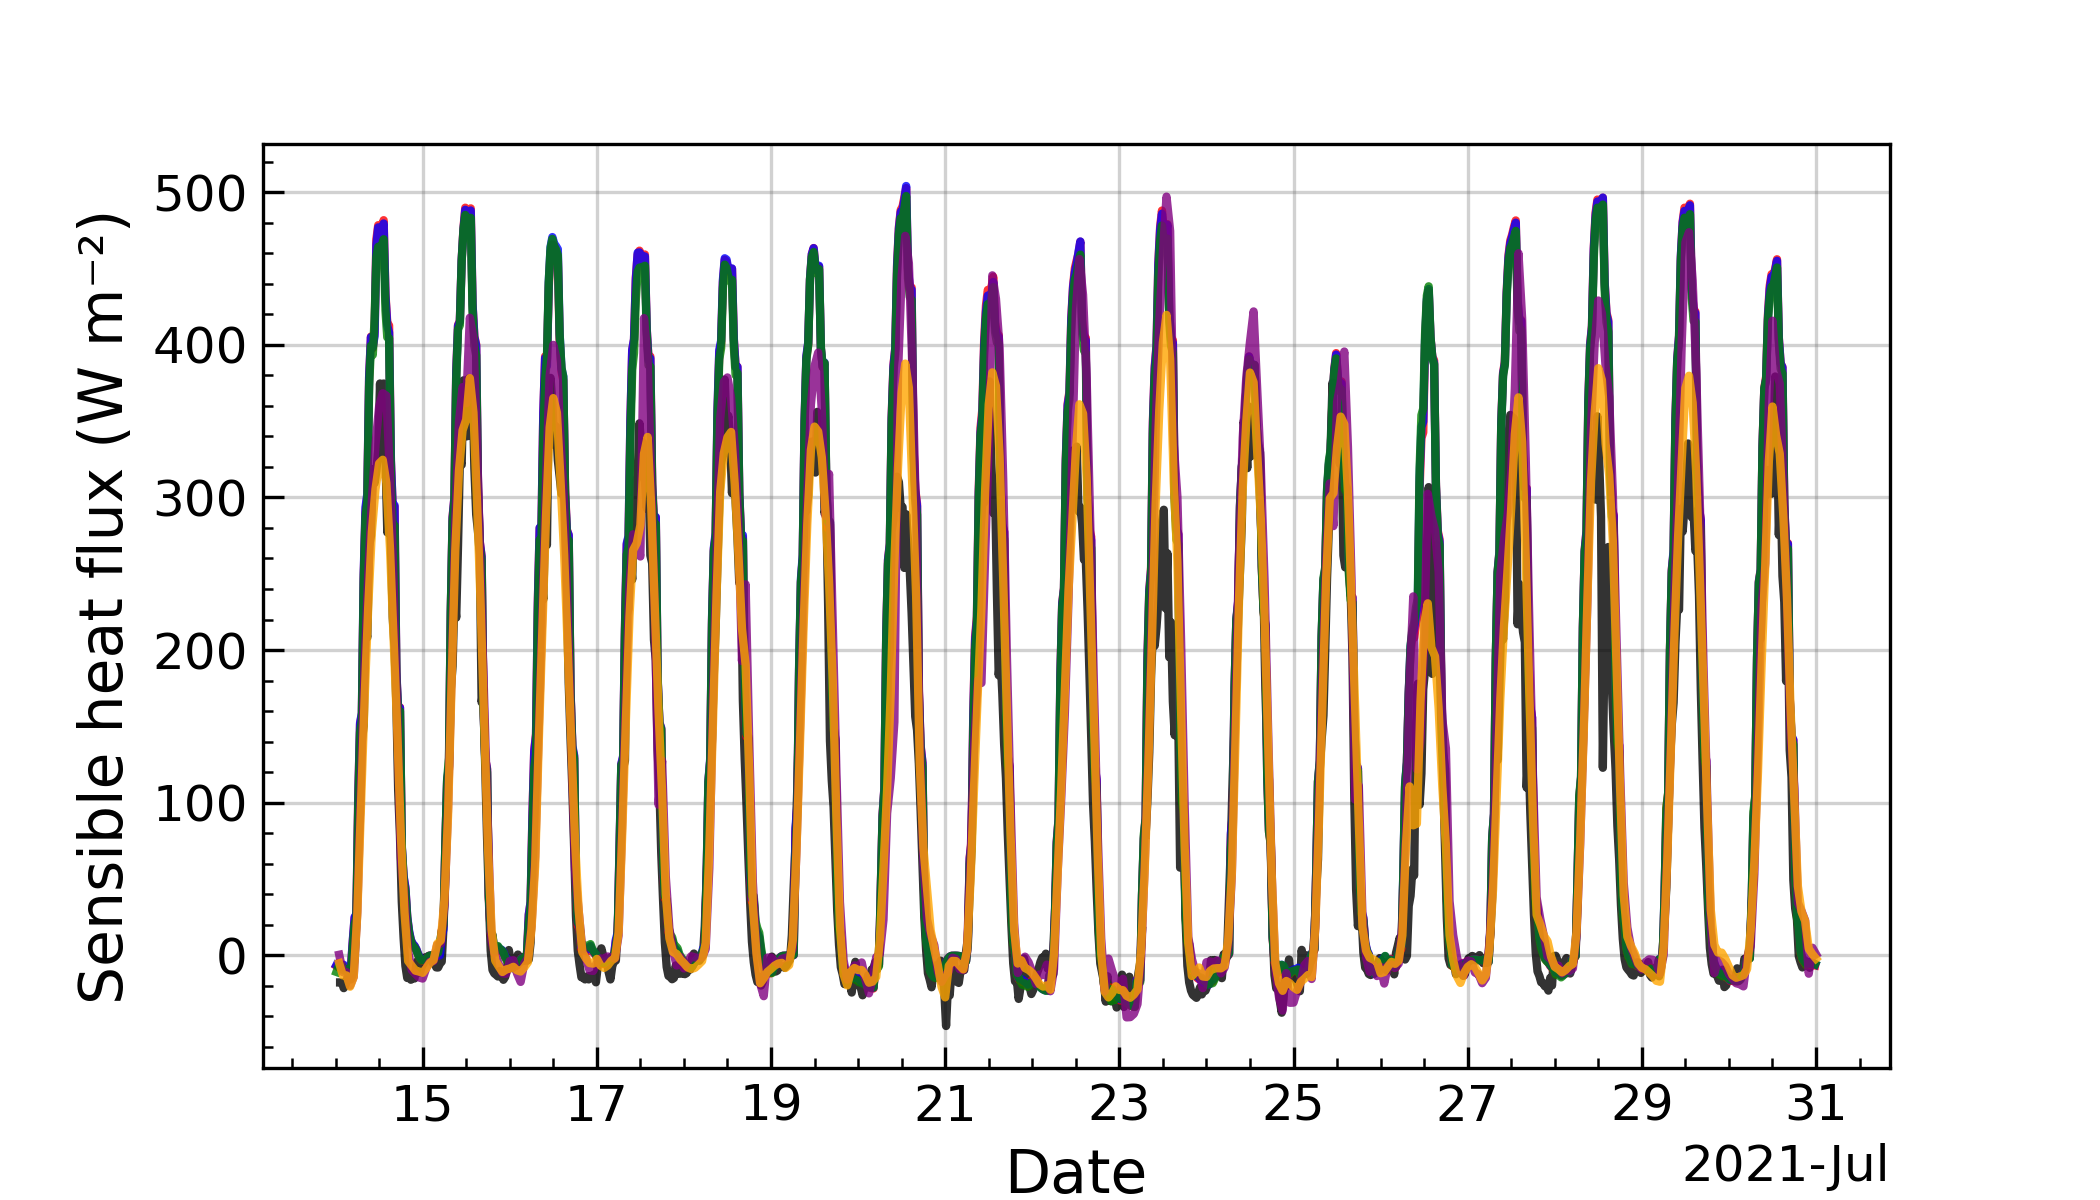
\includegraphics[width=\textwidth]{images/chap6/SOP_TS_DC/time_series_elsplans_sens.png}
        \end{subfigure} &
        \begin{subfigure}[t]{0.5\textwidth}
            \caption{Mean diurnal cycle of sensible heat flux\\(14-30 July - Els Plans)}
            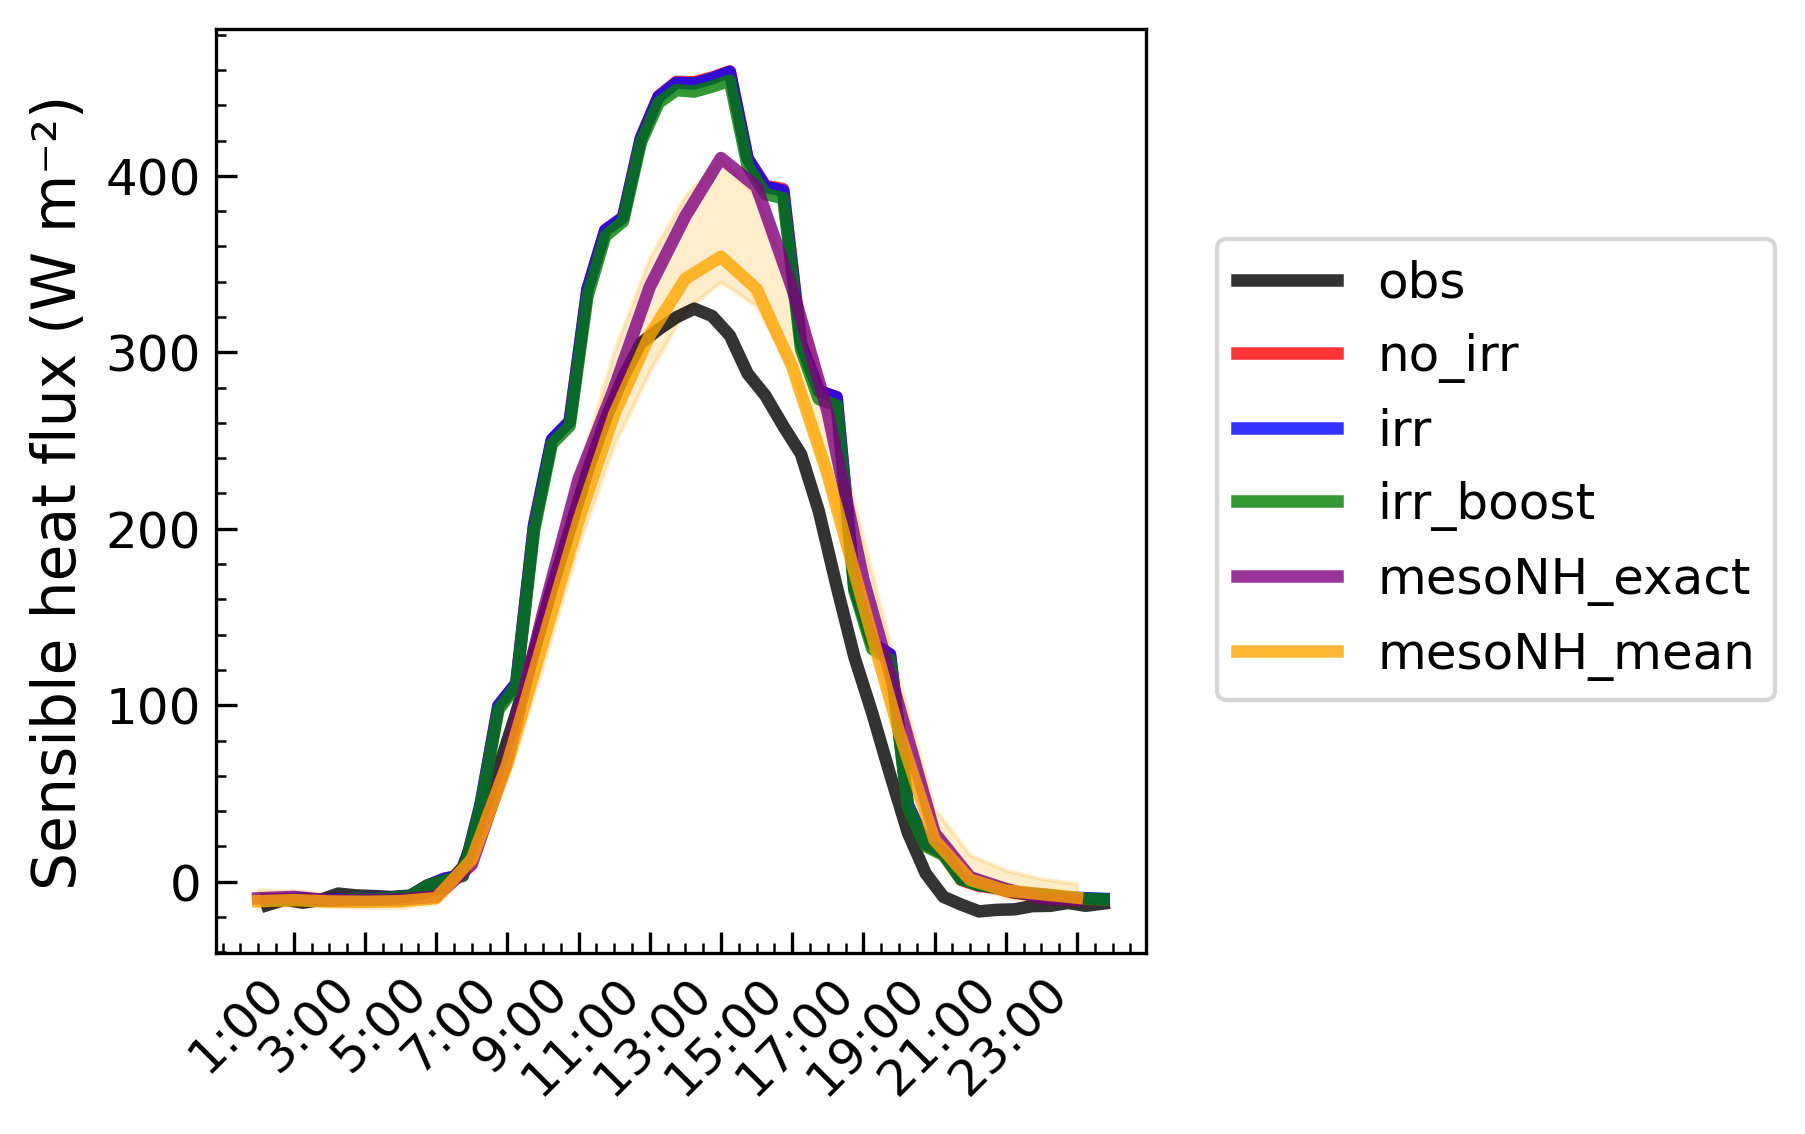
\includegraphics[width=\textwidth]{images/chap6/SOP_TS_DC/diurnal_cycle_elsplans_sens.png}
        \end{subfigure} \\
        \begin{subfigure}[t]{0.5\textwidth}
            \caption{2-meter temperature (Els Plans)}
            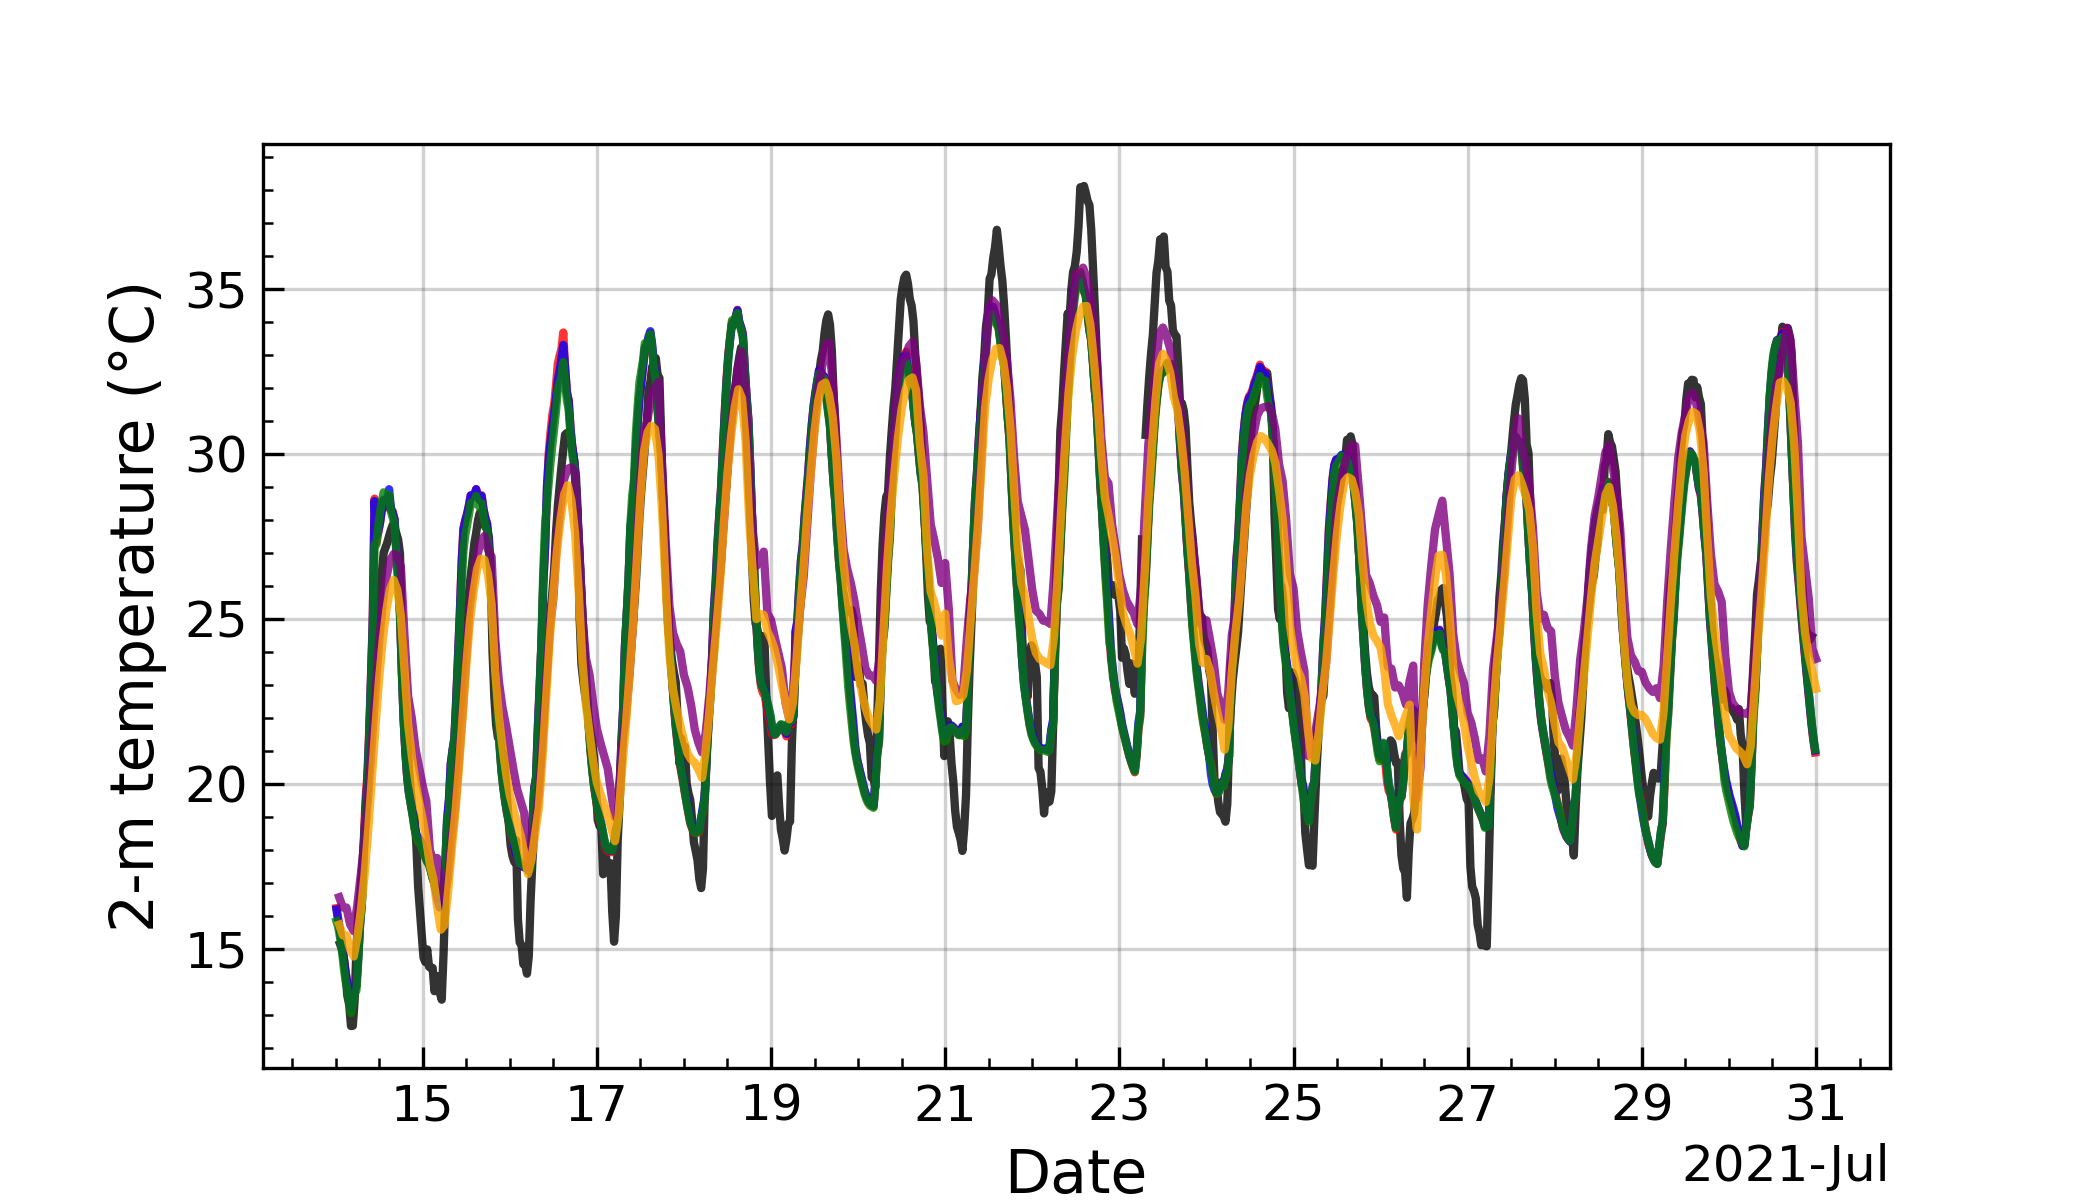
\includegraphics[width=\textwidth]{images/chap6/SOP_TS_DC/time_series_elsplans_t2m.png}
        \end{subfigure} &
        \begin{subfigure}[t]{0.5\textwidth}
            \caption{Mean diurnal cycle of 2-meter temperature\\(14-30 July - Els Plans)}
            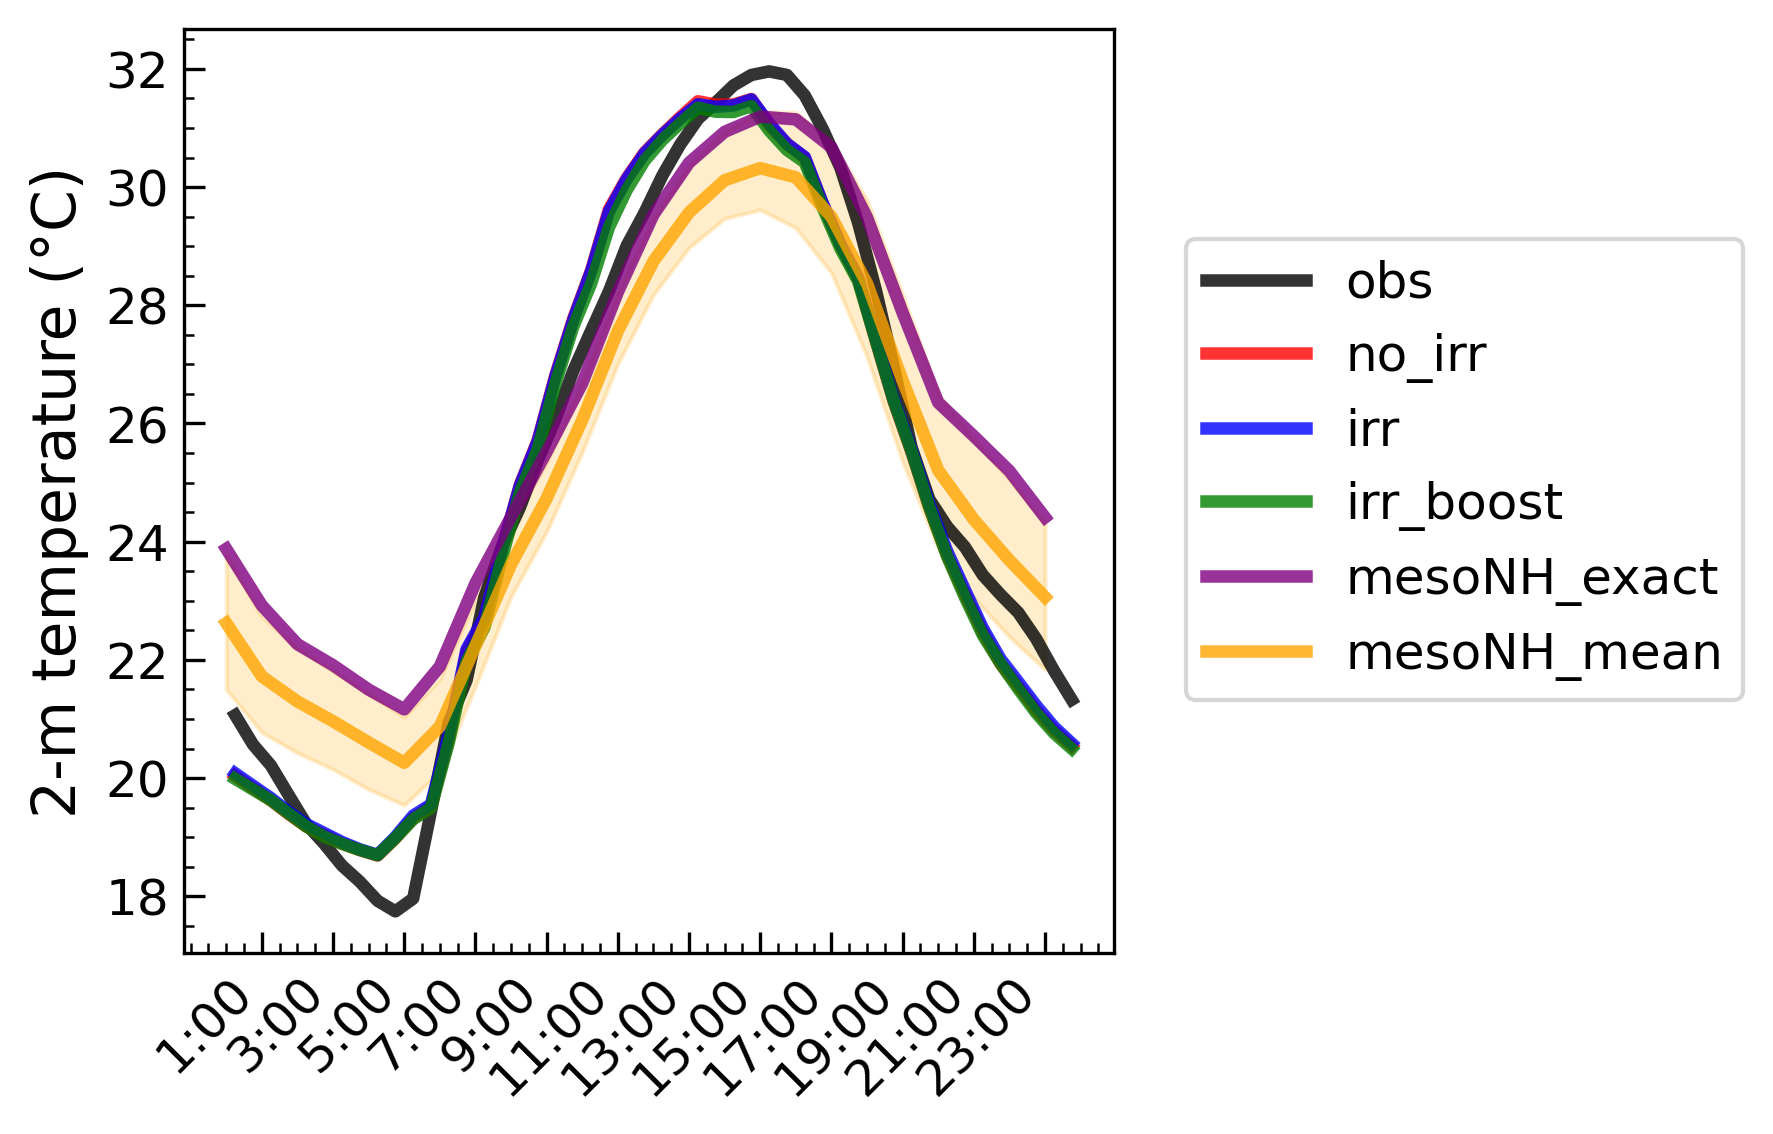
\includegraphics[width=\textwidth]{images/chap6/SOP_TS_DC/diurnal_cycle_elsplans_t2m.png}
        \end{subfigure} \\
        \begin{subfigure}[t]{0.5\textwidth}
            \caption{2-meter specific humidity (Els Plans)}
            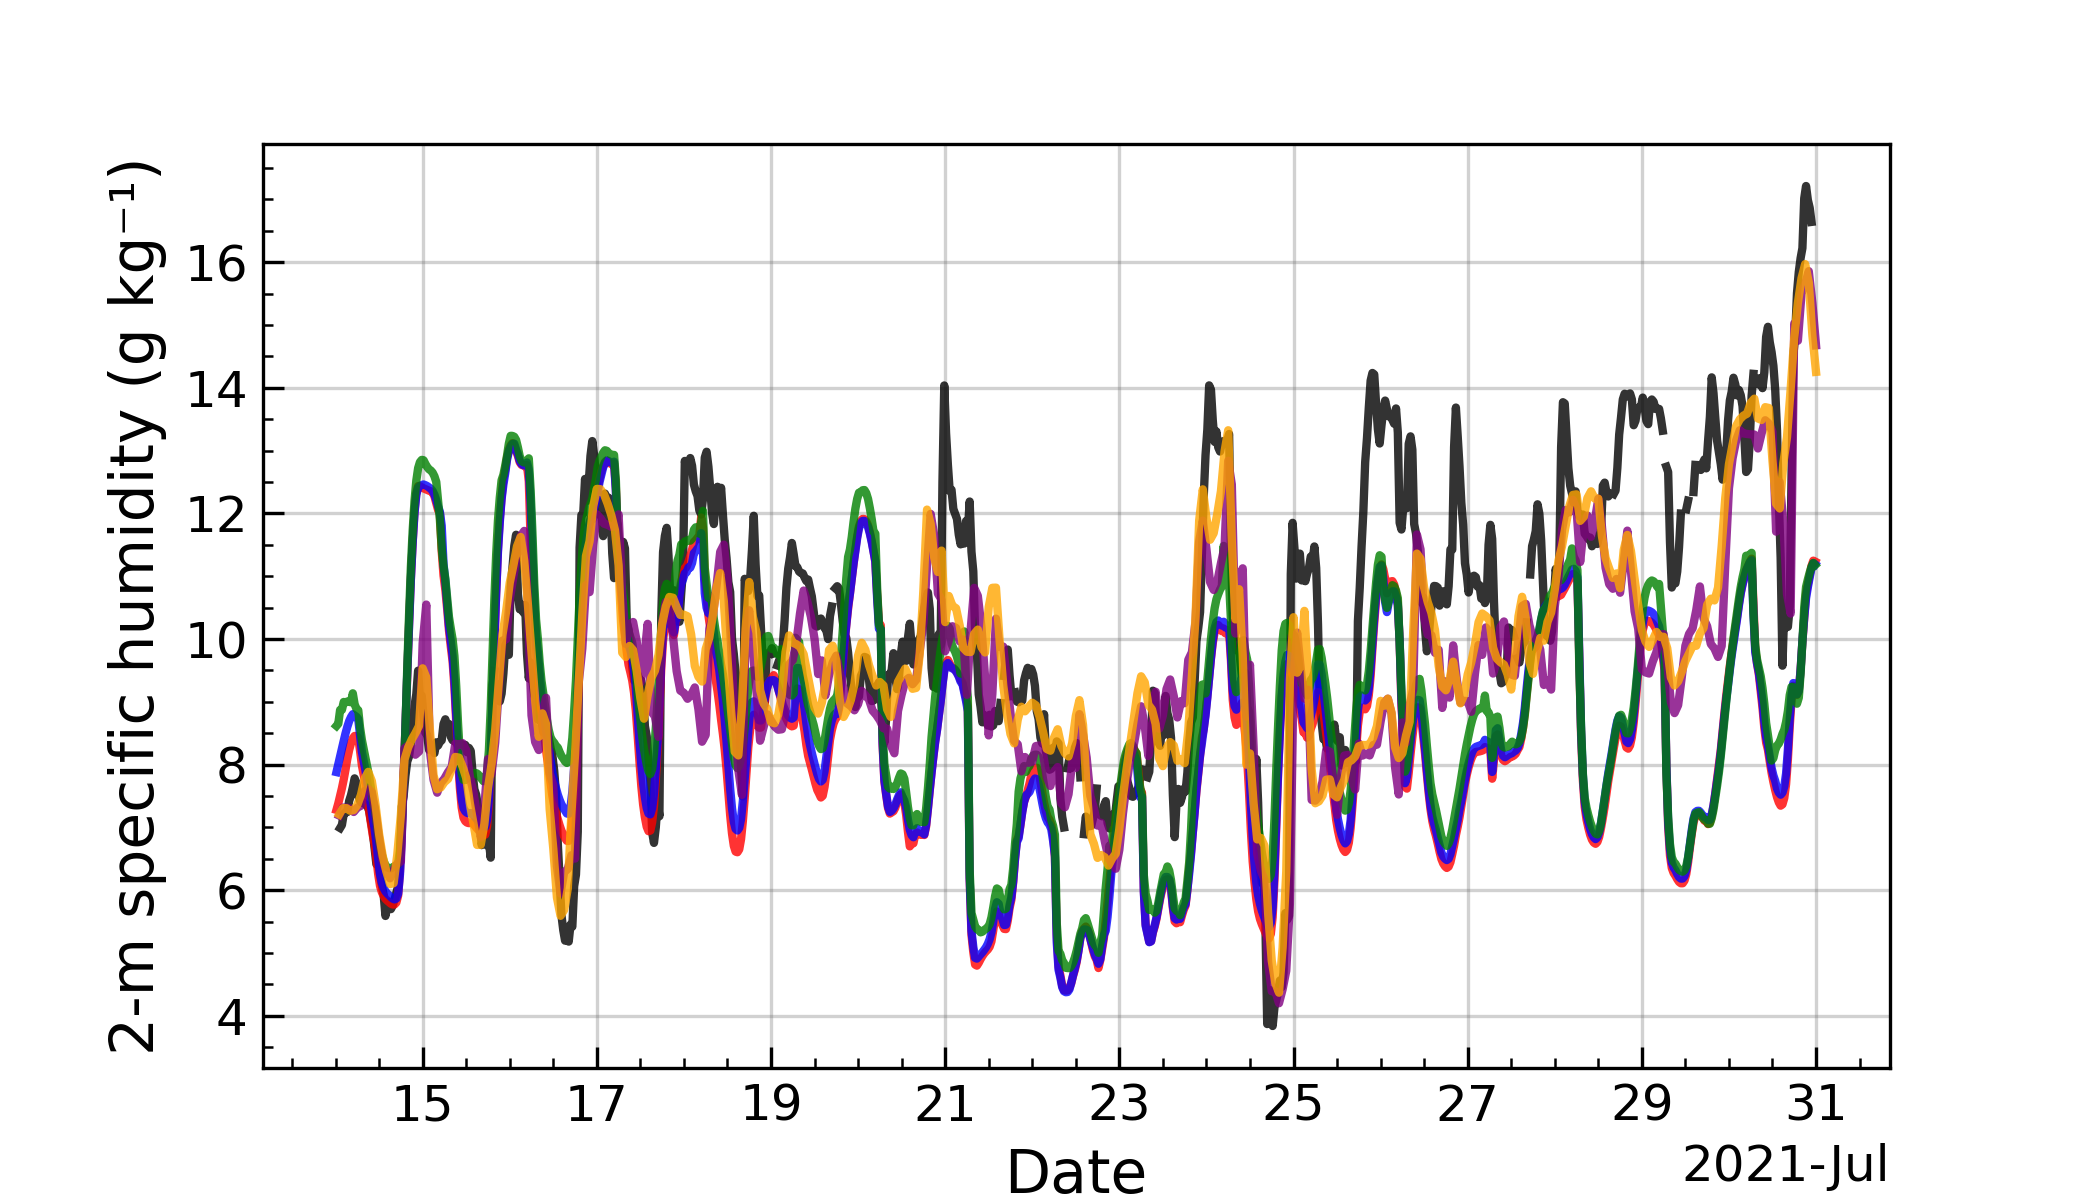
\includegraphics[width=\textwidth]{images/chap6/SOP_TS_DC/time_series_elsplans_q2m.png}
        \end{subfigure} &
        \begin{subfigure}[t]{0.5\textwidth}
            \caption{Mean diurnal cycle of 2-meter specific humidity\\(14-30 July - Els Plans)}
            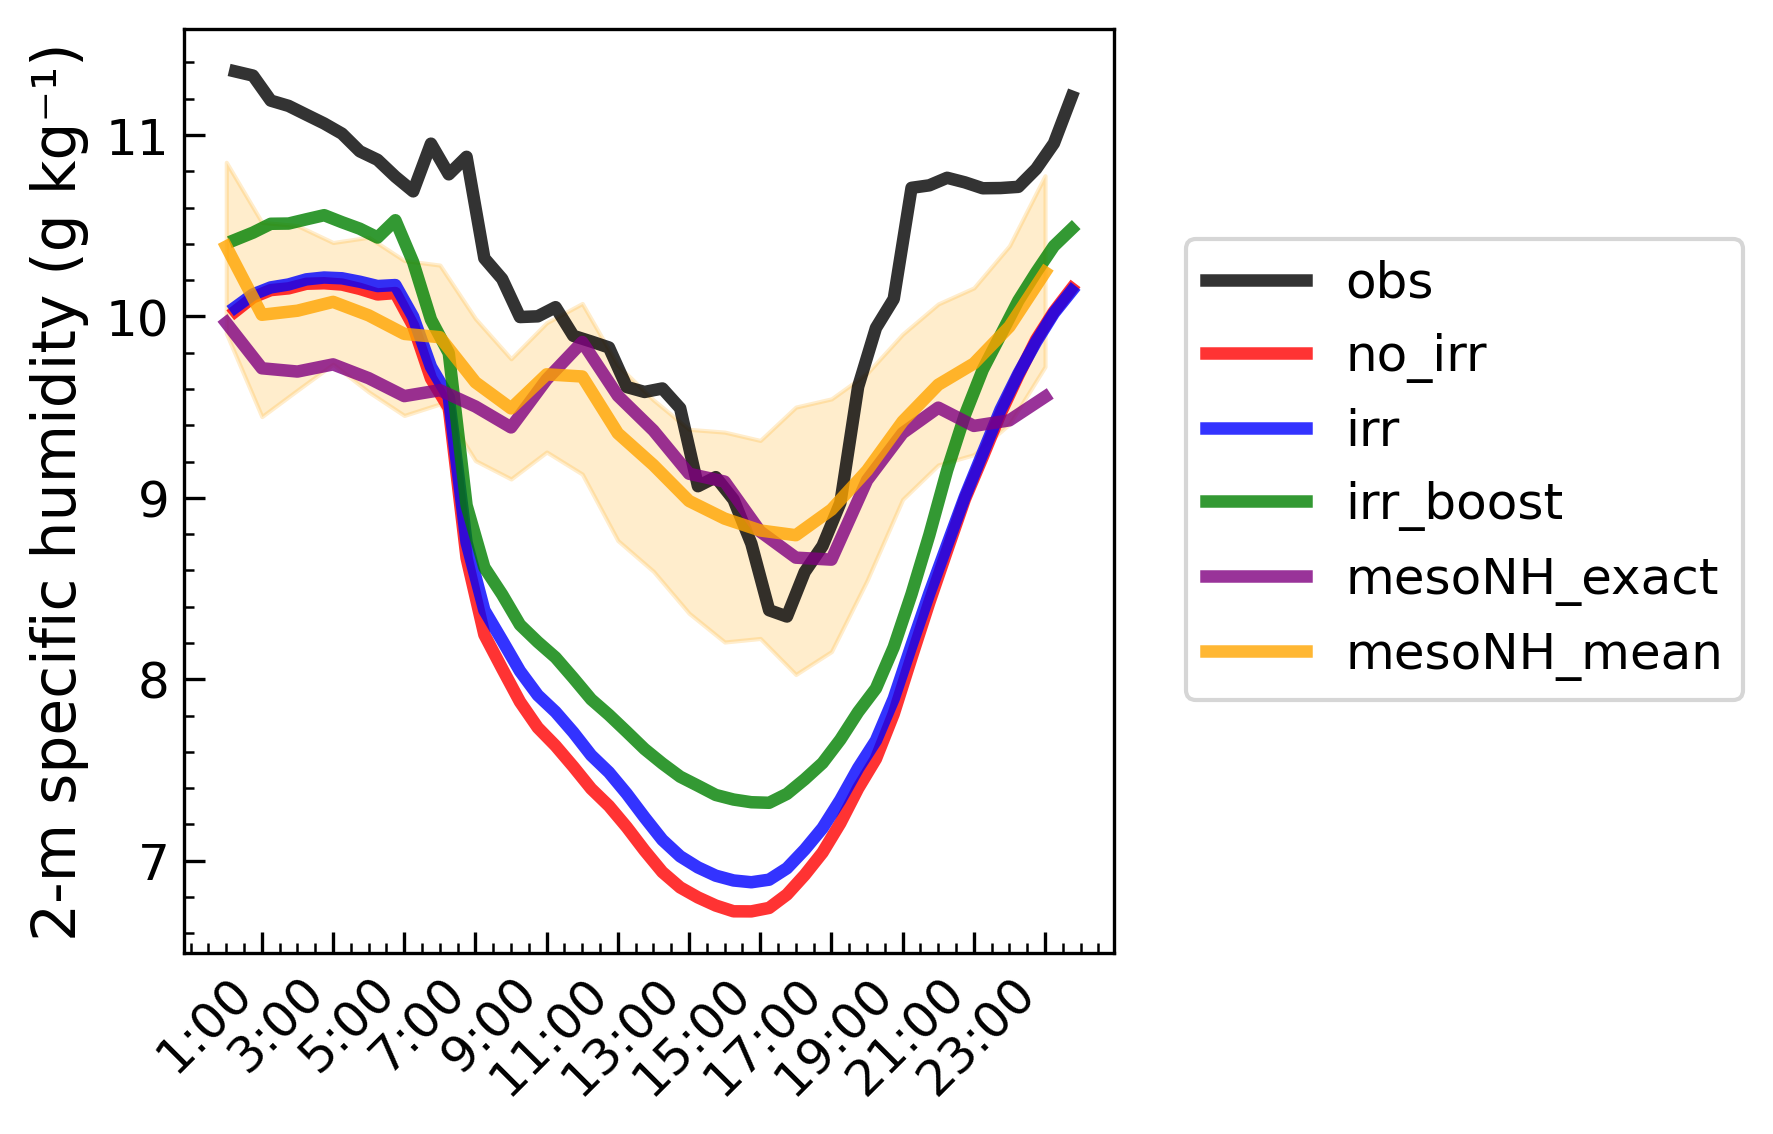
\includegraphics[width=\textwidth]{images/chap6/SOP_TS_DC/diurnal_cycle_elsplans_q2m.png}
        \end{subfigure}
    \end{tabular}
    \caption{Time series and mean diurnal cycle (14-30 July) of surface turbulent fluxes (a-d), temperature (e-f) and specific humidity (g-h) at Els Plans (rainfed site). The envelope for \mesomean represents the 25th and 75th percentiles of the distribution.}
    \label{fig:elsplans_surfacevars}
\end{figure}

\subsubsection*{Conclusions on near-surface variables}
The key takeaways from this comparison of near-surface variables over the SOP is that the irrigation parametrization can significantly improve the results at La Cendrosa, especially if irrigation demand is fully satisfied, as done in the \irrboost sensitivity experiment.
In particular, even if the observations cannot be matched perfectly, near-surface variables simulated by ICOLMDZOR are very close to the \mesomean values. Considering that the Meso-NH simulation is a relevant reference (ensured by the good performance of \mesoexact), it means that a good representation of grid-cell average values is achieved in the \irrboost simulation. 
In the second part of the SOP, a dry bias in ICOLMDZOR was identified, which is reduced but not entirely corrected by irrigation. Since this limitation is also visible at the rainfed site of Els Plans, and occurs simultaneously with a change in near-surface wind regime, it was hypothesized to be mainly the consequence of non-local processes, such as insufficient moisture advection over the LIAISE study area. The next section provides a study of the vertical structure of the ABL over two days, 15 July and 20 July, to investigate the differences between the first and second part of the SOP, and characterise the impact of irrigation and surface heterogeneities in these two different contexts.
%option:compléter sur les vents en disant qu'on n'est pas trop mauvais sur la moyenne (sauf vitesse à Els Plans) mais que ça cache beaucoup de variation selon les jours et heures ?

\clearpage

\section{Vertical structure of the atmosphere}
\label{sec:iop}

Out of the seven IOP days over which radiosoundings were conducted on both sites, two were selected (15 July and 20th) to further investigate the atmospheric behaviour of the ICOLMDZOR LAM and the impact of irrigation on the vertical structure of the ABL. 
15 July was selected as a representative IOP day for the beginning of the SOP, showing similarities with observed profiles on the 16 and 17 July. As the SOP progressed, 2-meter temperature increased and the wind regime became much more changeable, with more influence from the sea breeze circulation.
The three following IOP days (20, 21, 22 July) therefore presented different conditions, and 20 July was also selected to analyse the impacts of irrigation on the ABL in this other context.

\subsection{Observed and modelled surface conditions at La Cendrosa on IOP days}

The time series at La Cendrosa over both days (Fig. \ref{fig:iop_days_TS_surfvars}) clearly show that 20 July was a warmer and moister day than 15 July.
On 20 July, the observed latent heat flux is higher and the sensible heat flux lower, even presenting negative values in the afternoon.
While the wind direction and speed are rather stable on 15 July (westerly wind, lower than 3 m \persec), important variations are observed on 20 July.
The observed 10-meter wind in the morning is very low and mainly comes from the North-Northwest (NNW). 
In the afternoon, observations show a rapid change in wind direction to a southeasterly wind, associated with an increase in wind speed from less than 1 m \persec to more than 5 m \persec. That sudden variation is very likely associated with a complex regional circulation phenomenon, referred to as the \textit{marinada}. It results from the interaction of a sea breeze, bringing moist air from the Mediterranean sea, with the Catalan pre-coastal mountain range \citep{lunel_marinada_2024}, but is out of the scope of this study.

\hfill

In the models, the great performance of \mesoexact on both days must first be stressed, as it validates the Meso-NH simulation as a relevant reference to underestand the processes at play and evaluate ICOLMDZOR. 
Its only clear shortcomings are a warm bias at night visible on both days which disappears after sunrise (Fig. \ref{fig:iop_days_TS_surfvars}a-b), and an imbalance in the energy partitionning of turbulent fluxes on 15 July.
As mentionned in Section \ref{sec:sop}, at the beginning of the SOP, crops had recently been cut and plant transpiration was not at its usual level.
Since the models do not account for this information, the latent heat flux is overestimated and the sensible heat flux is underestimated (Fig. \ref{fig:iop_days_TS_energy}a, c). The same bias is visible with ICOLMDZOR in the \irrboost simulation. 
Similar figures are available for the Els Plans site in the appendix (Fig. \ref{fig:iop_days_TS_surfvars_elsplans} and \ref{fig:iop_days_TS_energy_elsplans}) which also confirm the general fidelity of the Meso-NH simulation to observations on both days.
While the Meso-NH simulation started from an initial state chosen to be as realistic as possible and focused on the domain of the LIAISE study area, the ICOLMDZOR simulation setup is not particularly tuned to reflect observed synoptic conditions, only relying on the lateral boundary conditions from ERA5. Considering this, obtaining a diurnal evolution that is similar to observations (and even more to \mesomean) for most surface variables on both days is already a satisfying performance. Yet, some limitations remain that must be taken acknowledged before analyzing the vertical structure of the atmosphere.

%LMDZ biases in t2m, q2m
At the surface, ICOLMDZOR presents a warm bias on 15 July that is partly reduced by irrigation, with a larger impact in \irrboost than in \irr, as expected. On 20 July, this bias is of smaller amplitude, and even suppressed in the day in the \irrboost simulation.
As previously noticed in general over the SOP, 2-meter specific humidity is overestimated by ICOLMDZOR at night, but decreases during the day, which is not very realistic at La Cendrosa. On 15 July, \irrboost remains slightly above observed and Meso-NH values during the day but on 20 July, daytime specific humidity is underestimated.
This may partly be explained by the differences in latent heat flux between the two days mentioned above (overestimation on 15 July and underestimation on 20 July).
However, despite \mesomean having the same surface fluxes as \irrboost, and very close values of 2-meter temperature, it does not present the same biases in 2-meter specific humidity at La Cendrosa (nor at Els Plans, Fig. \ref{fig:iop_days_TS_surfvars_elsplans} and \ref{fig:iop_days_TS_energy_elsplans}).
As conjectured in Section \ref{sec:sop}, near-surface humidity seems to be influenced by non-local processes on 20 July and the following days, which suggests an incorrect moisture advection in the ICOLMDZOR simulations. 
The low-level wind simulated by ICOLMDZOR matches very well with observations and \mesomean on 15 July, but does not reproduce the multiple direction and wind speed changes on 20 July. In particular, in the morning, ICOLMDZOR simulates an increasingly stronger wind from the South-Southeast (SSE), while observations and \mesoexact show NNW weak winds, and \mesomean exhibits low winds of changing directions, with a large envelope comprising northeasterly to southerly winds. This demonstrates the complex situation on 20 July, which cannot be fully captured by ICOLMDZOR, and will be further highlighted in Section \ref{sec:heterogeneities} and Fig. \ref{fig:iop_days_winds}.

The downward longwave radiation flux (LW down, Fig. \ref{fig:iop_days_TS_energy}g-h) summarises several differences between 15 July and 20 July. 
15 July has a smaller LW down flux since the atmosphere is cooler and drier, and ICOLMDZ overestimates it because of a warm bias. In \irrboost this warm bias is much smaller, but specific humidity is overestimated so overall, the bias in LW down is only slightly reduced. 
On 20 July, ICOLMDZOR presents a smaller warm bias (almost no bias for \irrboost) but a strong dry bias, leading to an underestimation of LW down. 
This analysis remains very simplified and assumes that some of the characteristics of near-surface variables can be extented to the rest of the ABL. The comparison of vertical profiles to radiosoundings at 12UTC presented in the next section provides further insight into the behaviour of the atmosphere on these two days.

%todo:figure of winds at 12UTC (10m and 850hPa) in LMDZ ? (déjà mesoNH en bas, sur 4 niveaux...)

%Fig : surface variables Cendrosa
\begin{figure}[hbtp]
    \centering
    \begin{tabular}{cc}
        %t2m, q2m
        \begin{subfigure}[t]{0.5\textwidth}
            \caption{2-meter temperature\\(15 July - La Cendrosa)}
            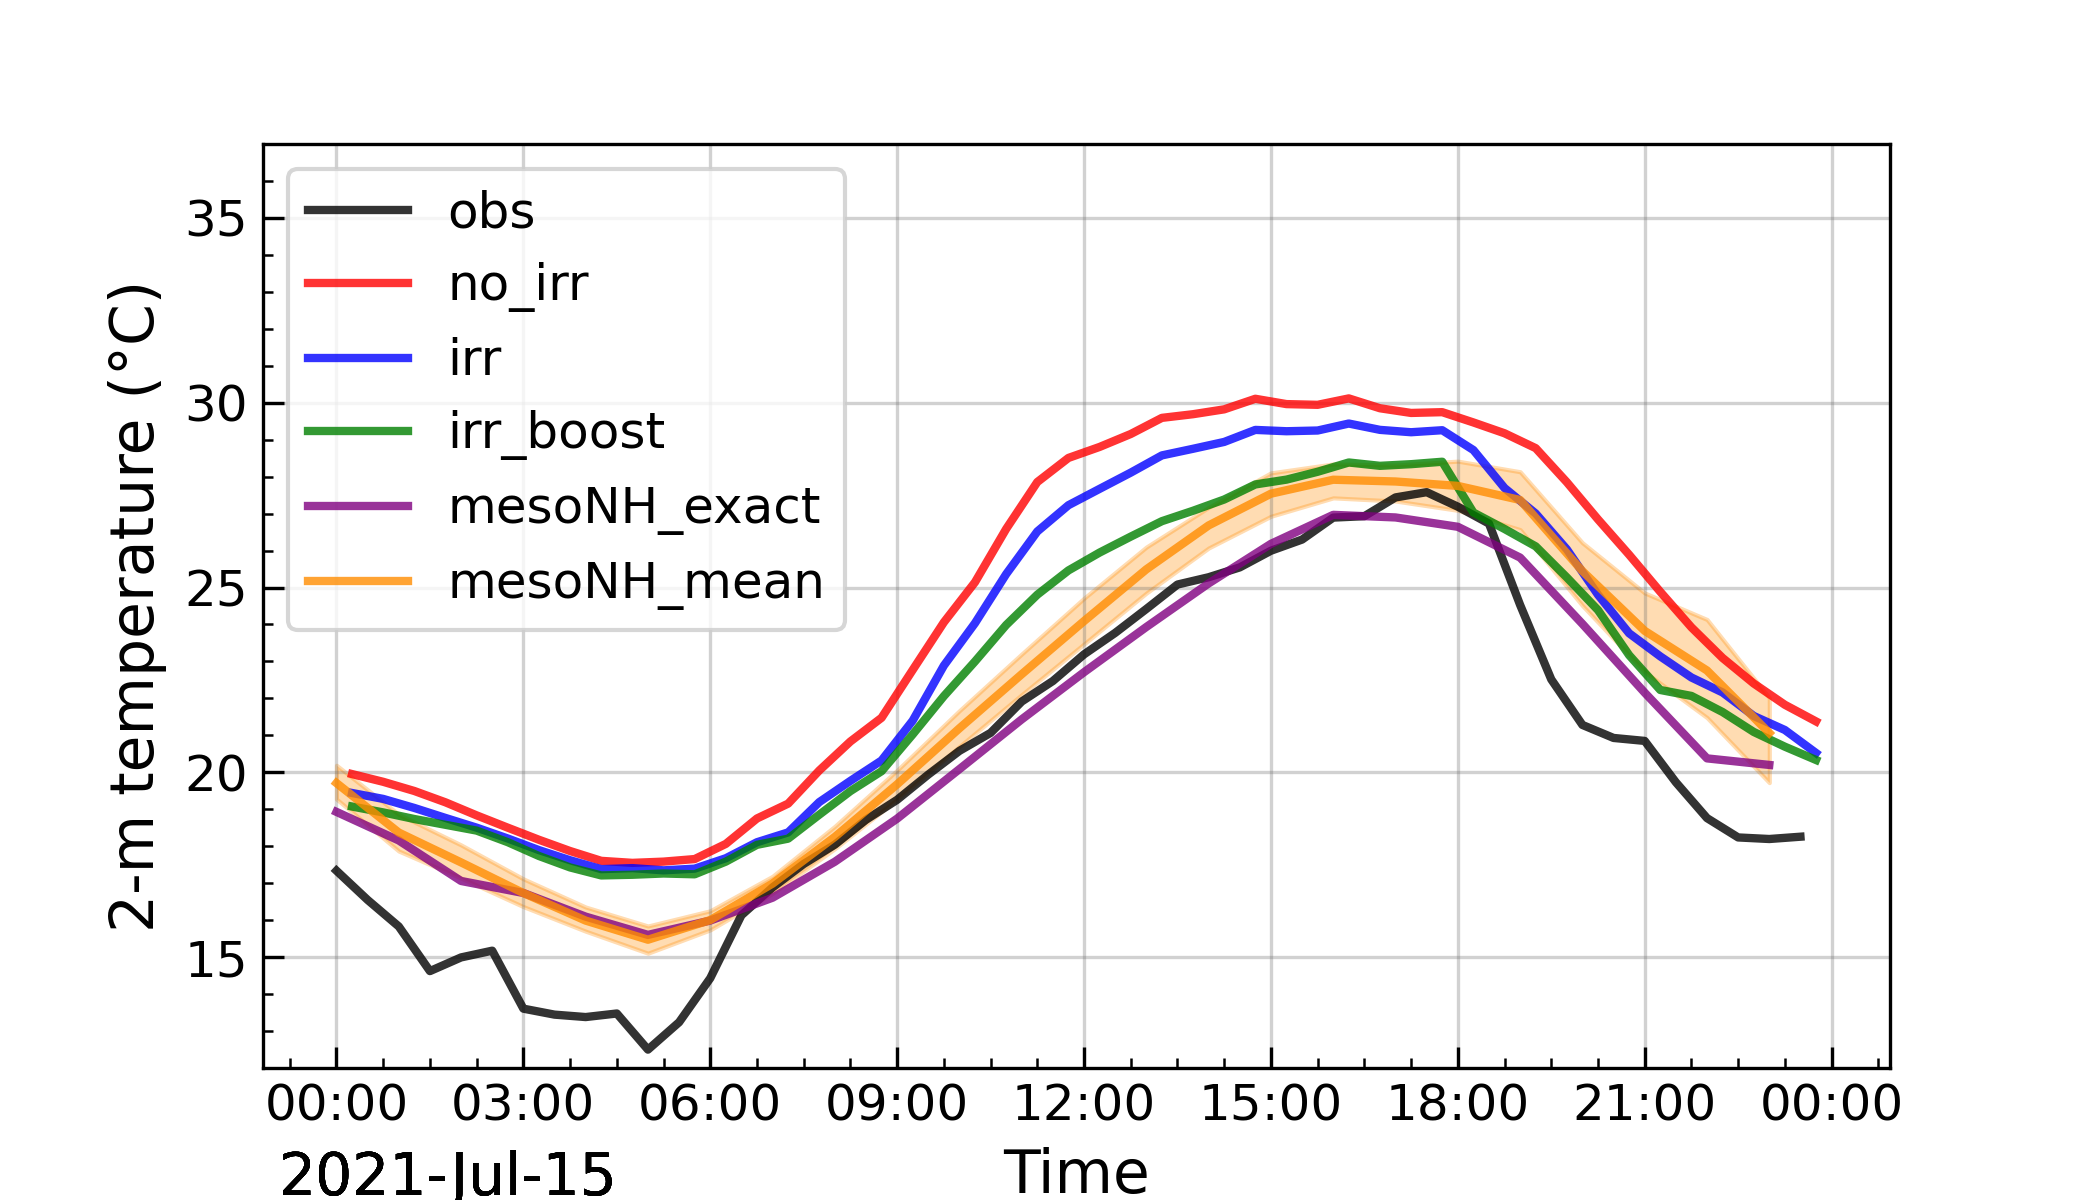
\includegraphics[width=\textwidth]{images/chap6/IOP_TS/TS_2021-07-15_cendrosa_t2m.png}
        \end{subfigure} &
        \begin{subfigure}[t]{0.5\textwidth}
            \caption{2-meter temperature\\(20 July - La Cendrosa)}
            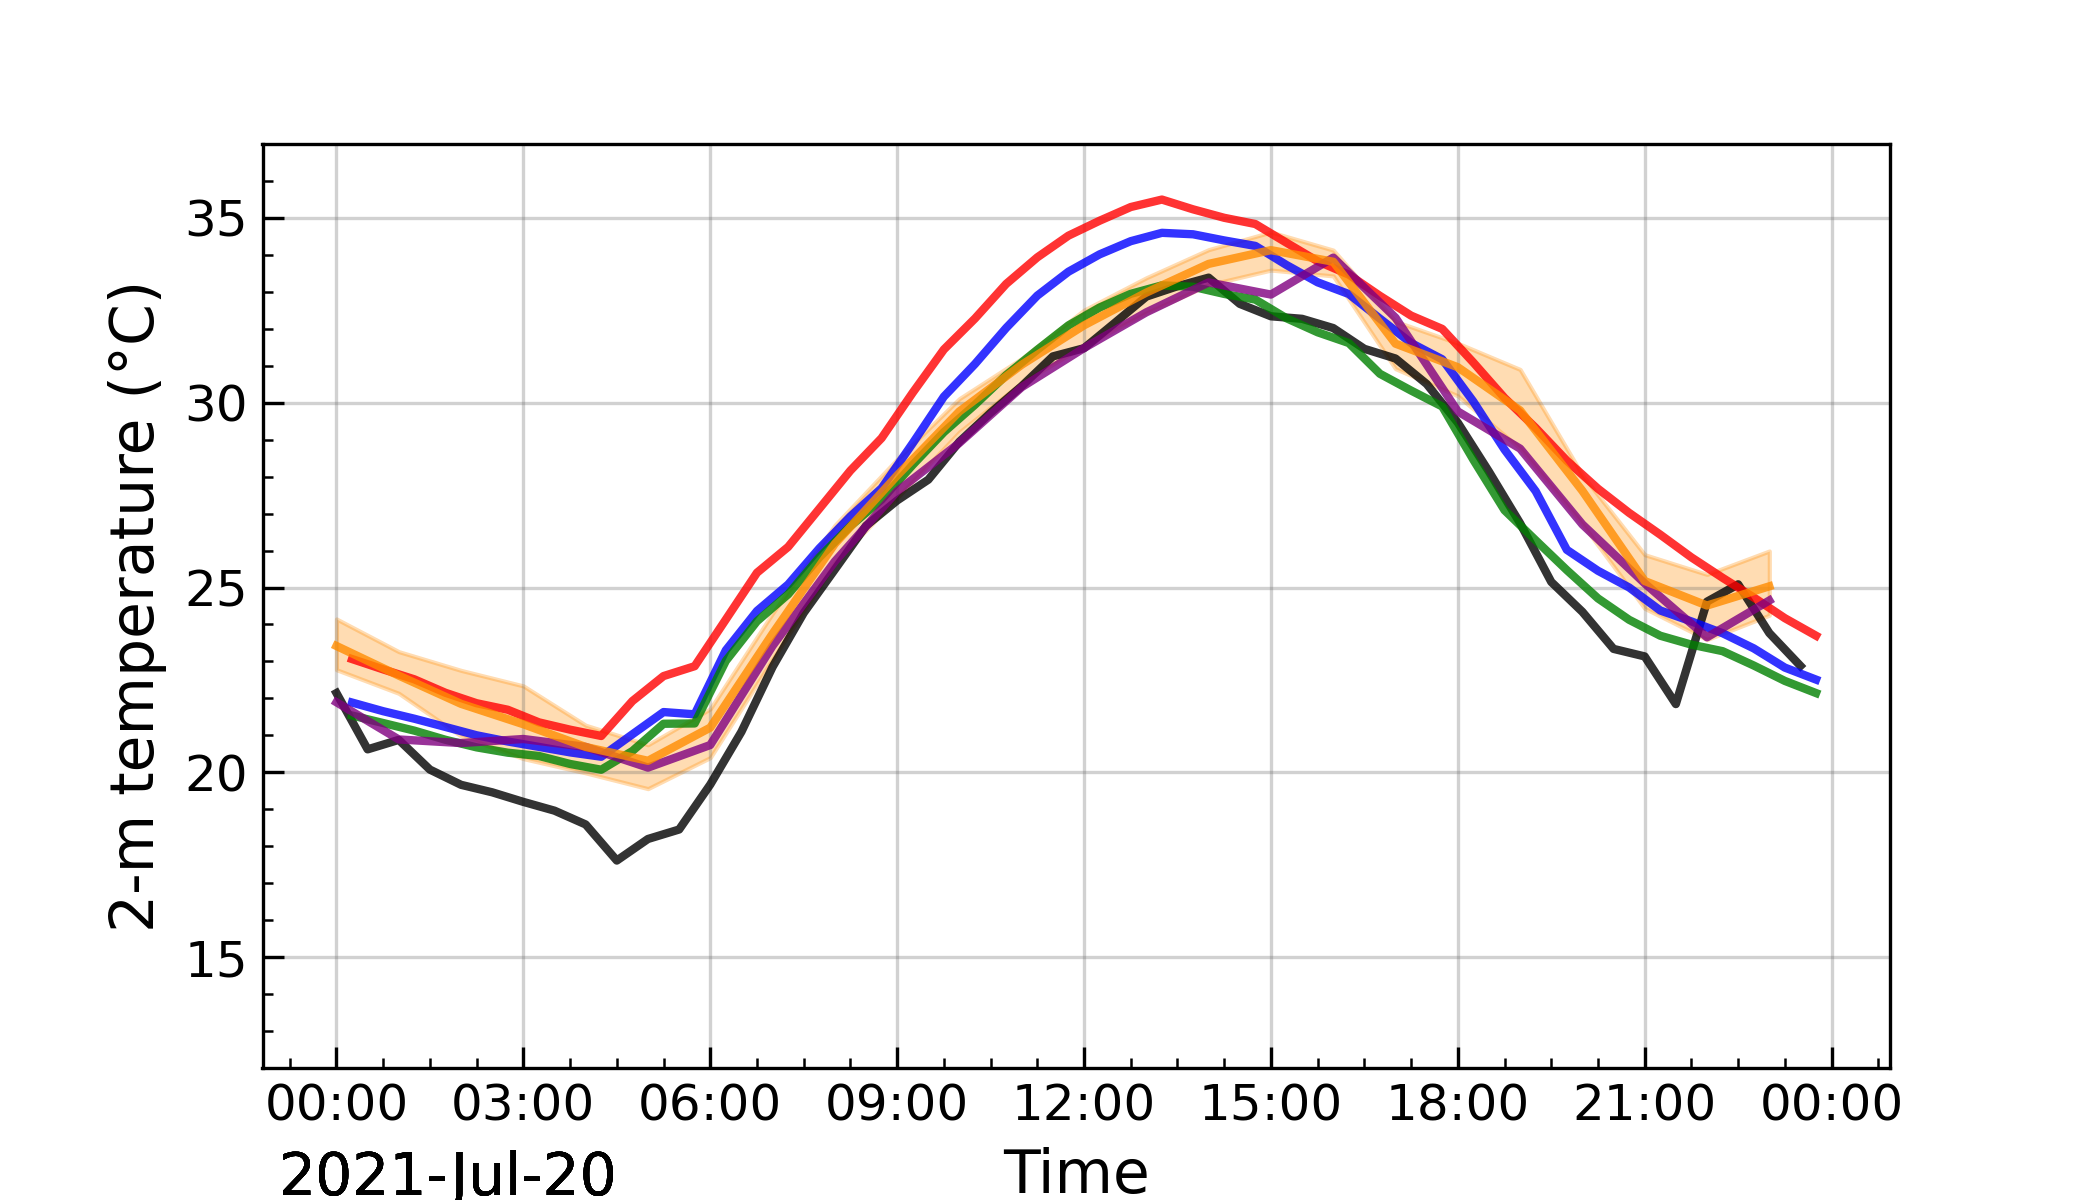
\includegraphics[width=\textwidth]{images/chap6/IOP_TS/TS_2021-07-20_cendrosa_t2m.png}
        \end{subfigure} \\
        \begin{subfigure}[t]{0.5\textwidth}
            \caption{2-meter specific humidity\\(15 July - La Cendrosa)}
            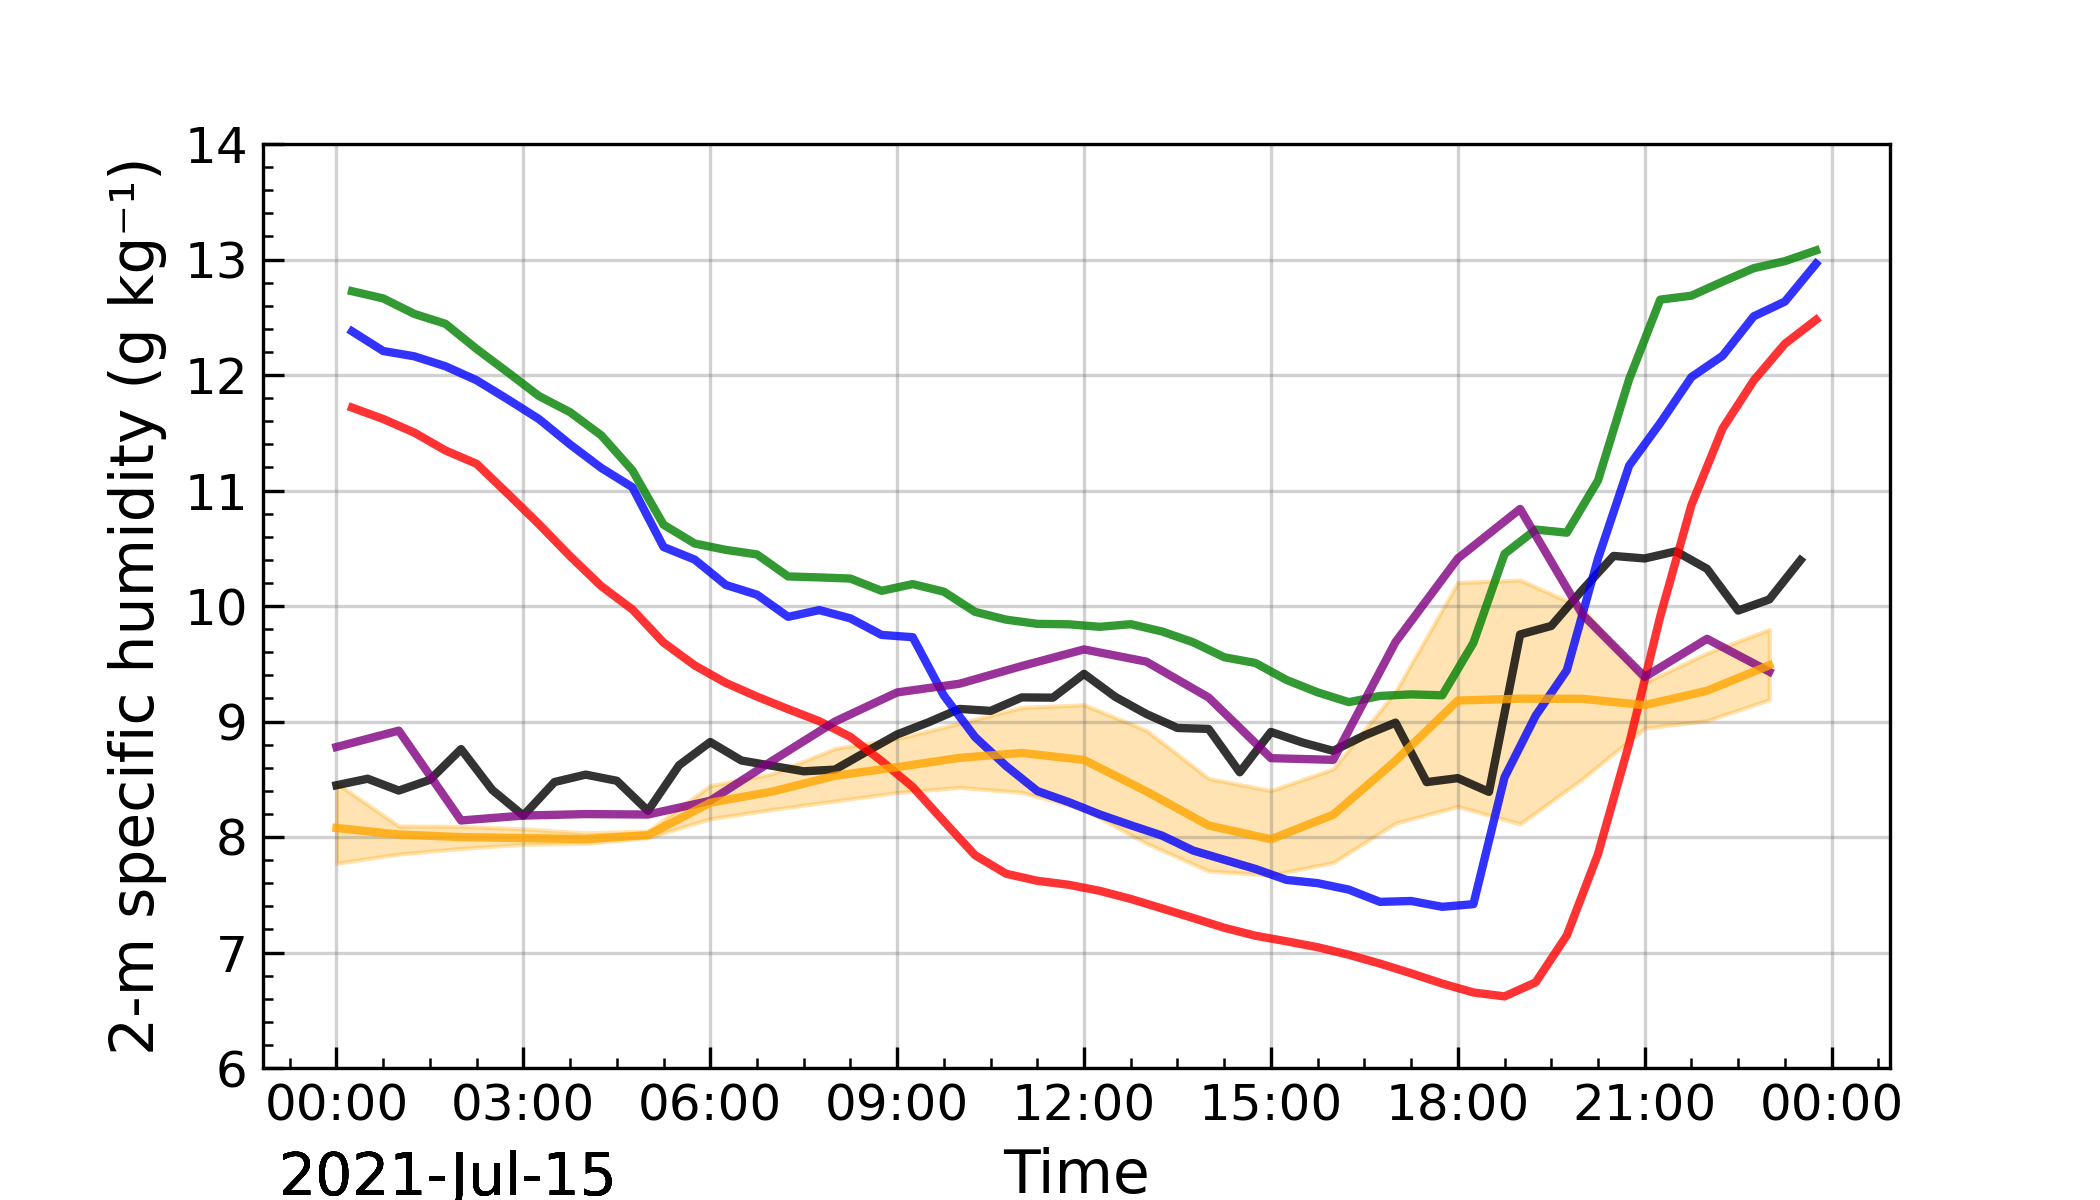
\includegraphics[width=\textwidth]{images/chap6/IOP_TS/TS_2021-07-15_cendrosa_q2m.png}
        \end{subfigure} &
        \begin{subfigure}[t]{0.5\textwidth}
            \caption{2-meter specific humidity\\(20 July - La Cendrosa)}
            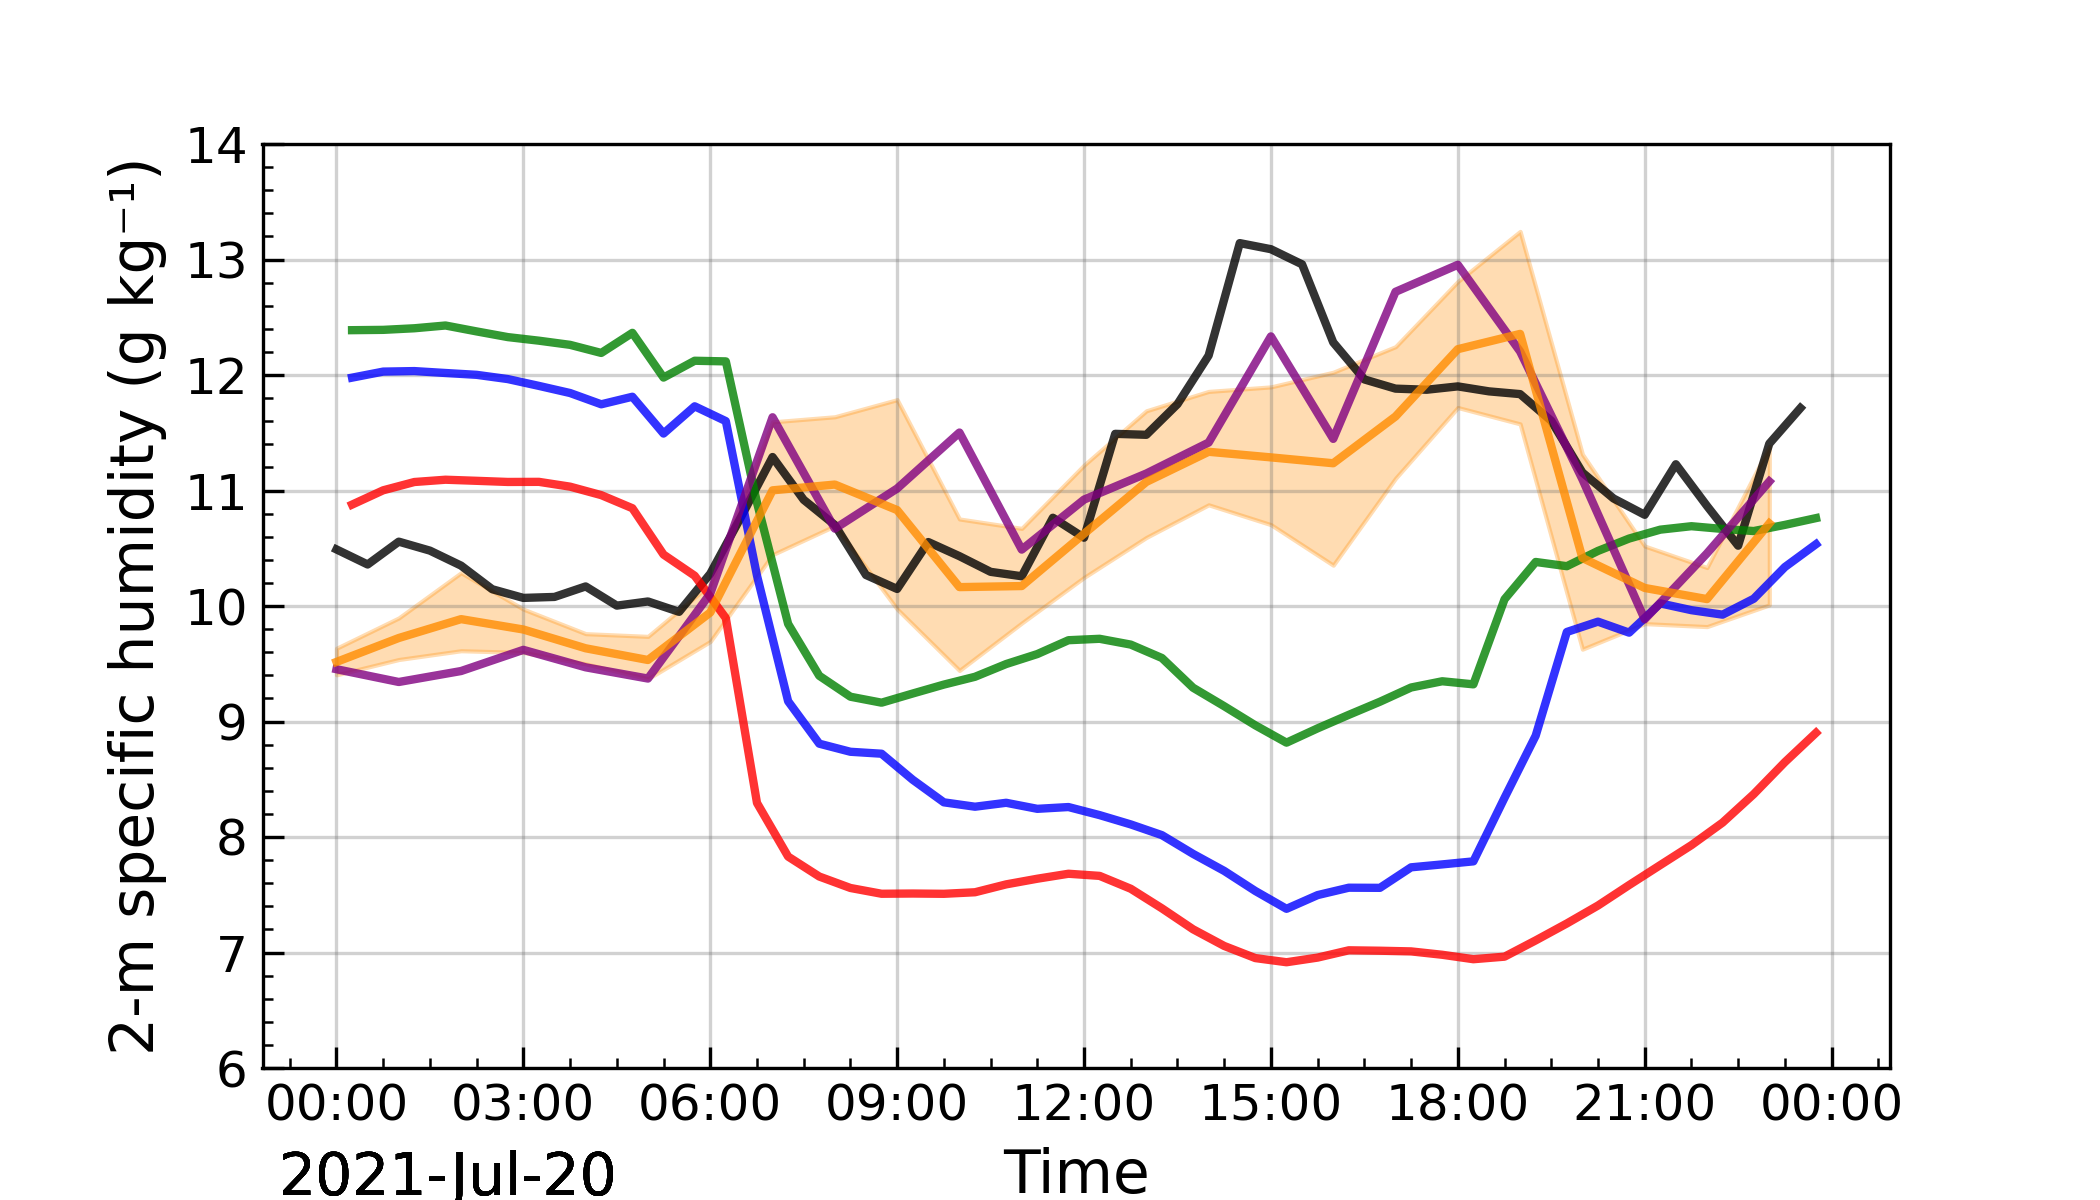
\includegraphics[width=\textwidth]{images/chap6/IOP_TS/TS_2021-07-20_cendrosa_q2m.png}
        \end{subfigure} \\

        %turb fluxes
        \begin{subfigure}[t]{0.5\textwidth}
            \caption{10-meter wind speed\\(15 July - La Cendrosa)}
            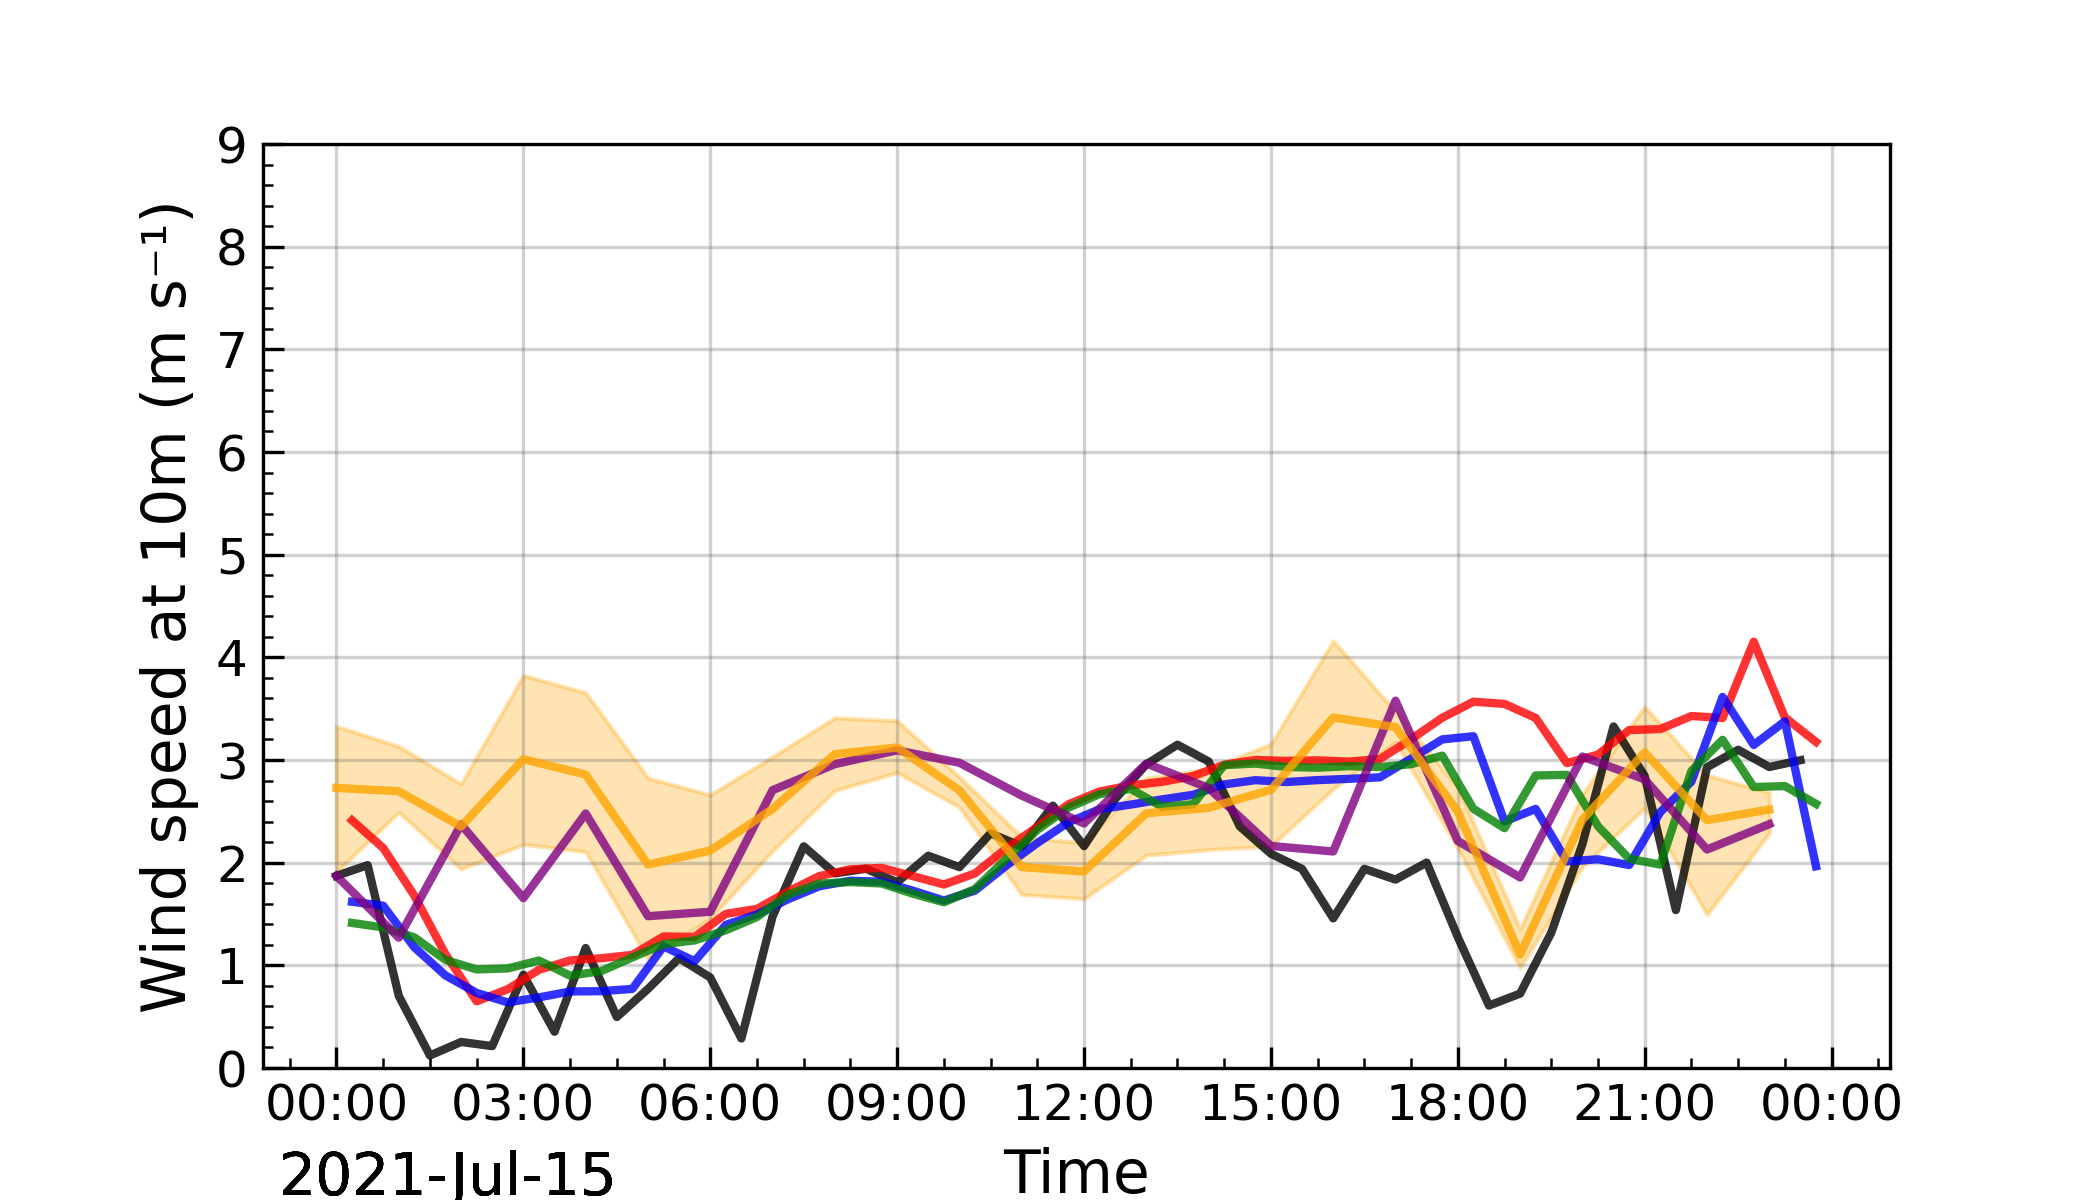
\includegraphics[width=\textwidth]{images/chap6/IOP_TS/TS_2021-07-15_cendrosa_wind_speed_10m.png}
        \end{subfigure} &
        \begin{subfigure}[t]{0.5\textwidth}
            \caption{10-meter wind speed\\(20 July - La Cendrosa)}
            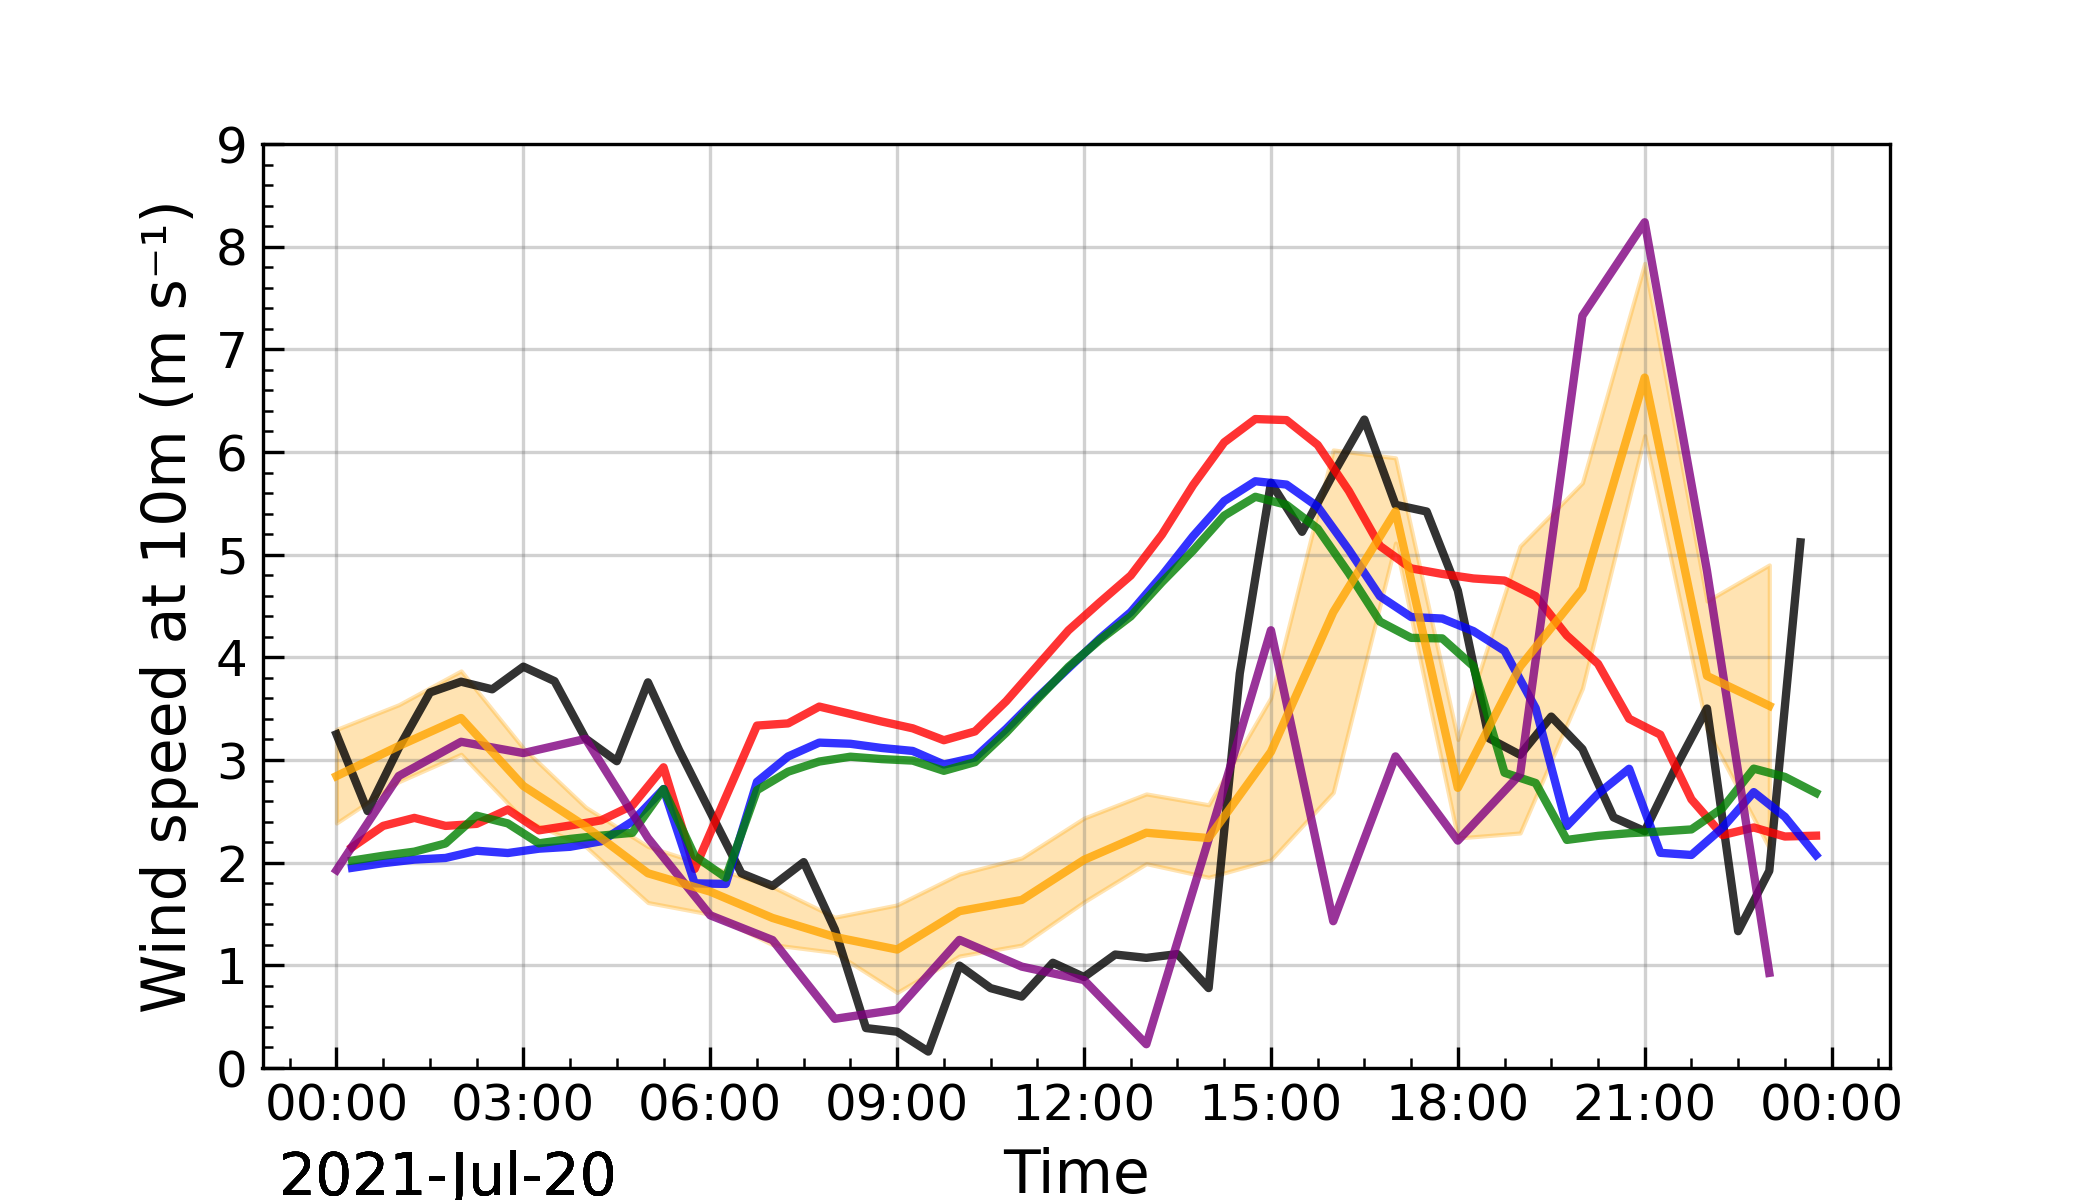
\includegraphics[width=\textwidth]{images/chap6/IOP_TS/TS_2021-07-20_cendrosa_wind_speed_10m.png}
        \end{subfigure} \\
        \begin{subfigure}[t]{0.5\textwidth}
            \caption{10-meter wind direction\\(15 July - La Cendrosa)}
            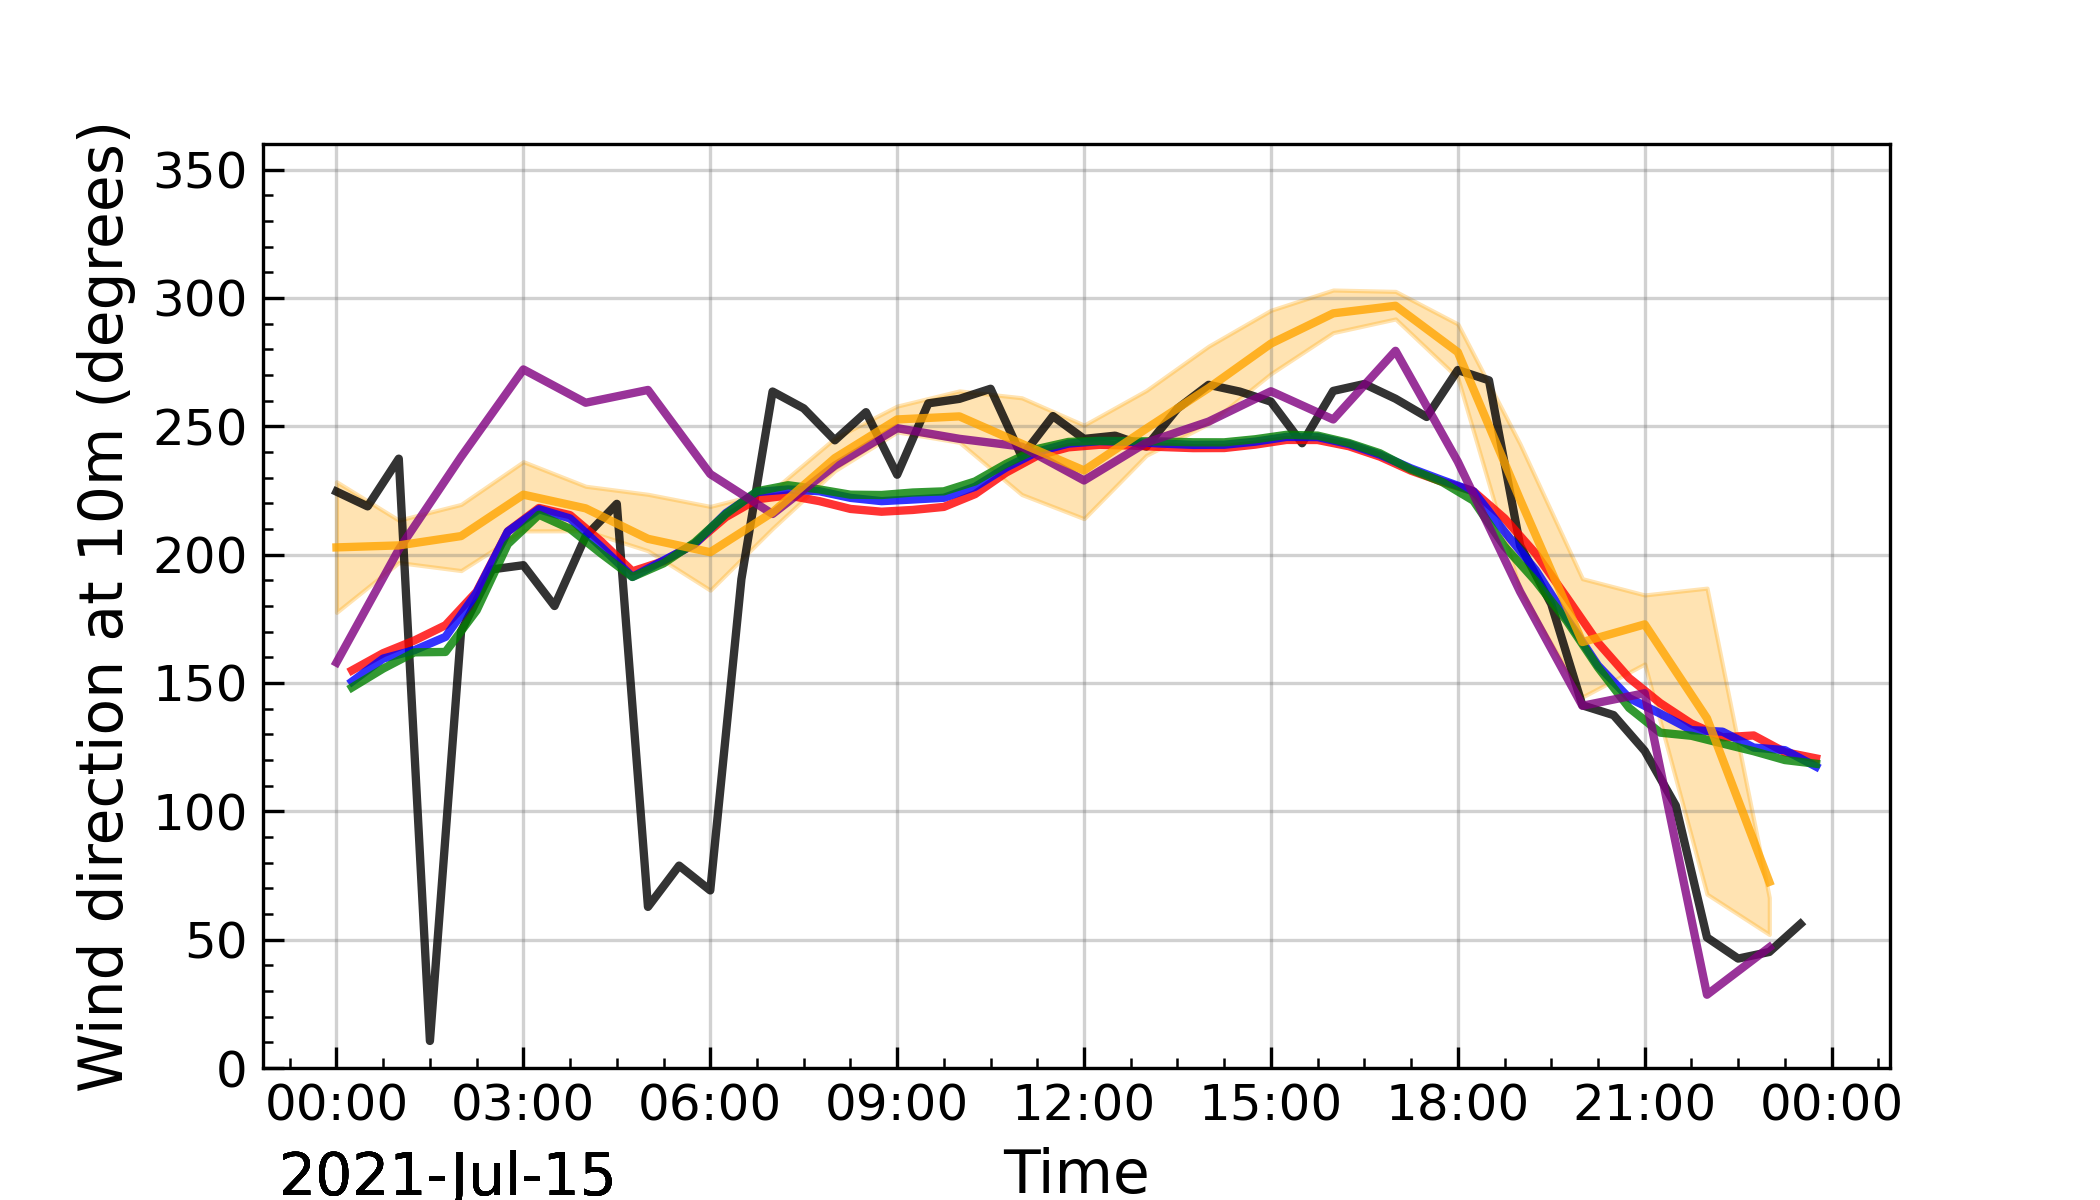
\includegraphics[width=\textwidth]{images/chap6/IOP_TS/TS_2021-07-15_cendrosa_wind_direction_10m.png}
        \end{subfigure} &
        \begin{subfigure}[t]{0.5\textwidth}
            \caption{10-meter wind direction\\(20 July - La Cendrosa)}
            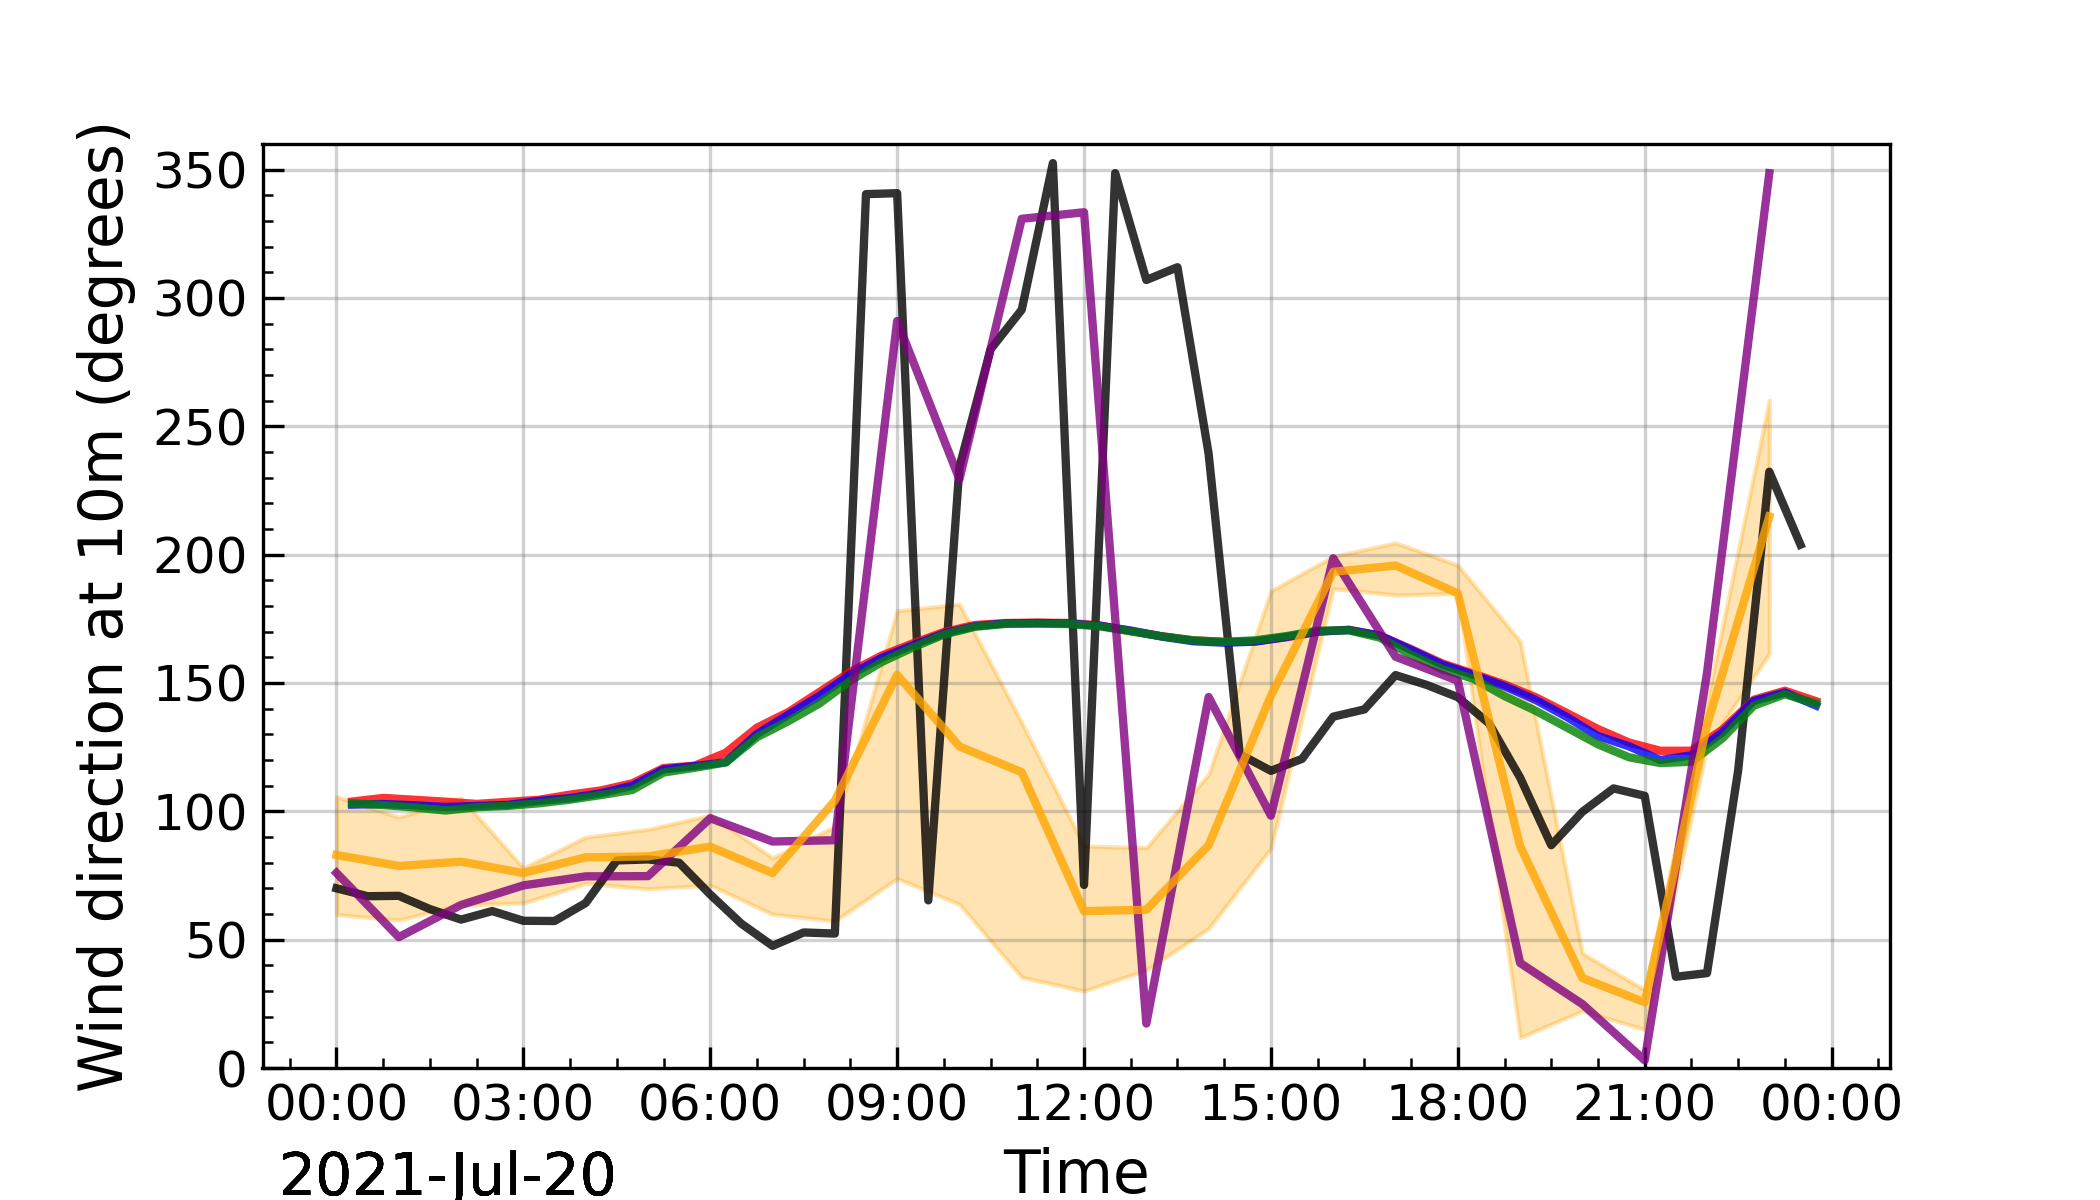
\includegraphics[width=\textwidth]{images/chap6/IOP_TS/TS_2021-07-20_cendrosa_wind_direction_10m.png}
        \end{subfigure} \\
    \end{tabular}
    \caption{Evolution of 2-m temperature (a-b), 2-m specific humidity (c-d), 10-m wind speed (e-f) and direction (g-h) at La Cendrosa on 15 and 20 July.}
    \label{fig:iop_days_TS_surfvars}
\end{figure}

%Fig : energy fluxes Cendrosa
\begin{figure}[hbtp]
    \centering
    \begin{tabular}{cc}
        %turb fluxes
        \begin{subfigure}[t]{0.5\textwidth}
            \caption{Latent heat flux\\(15 July - La Cendrosa)}
            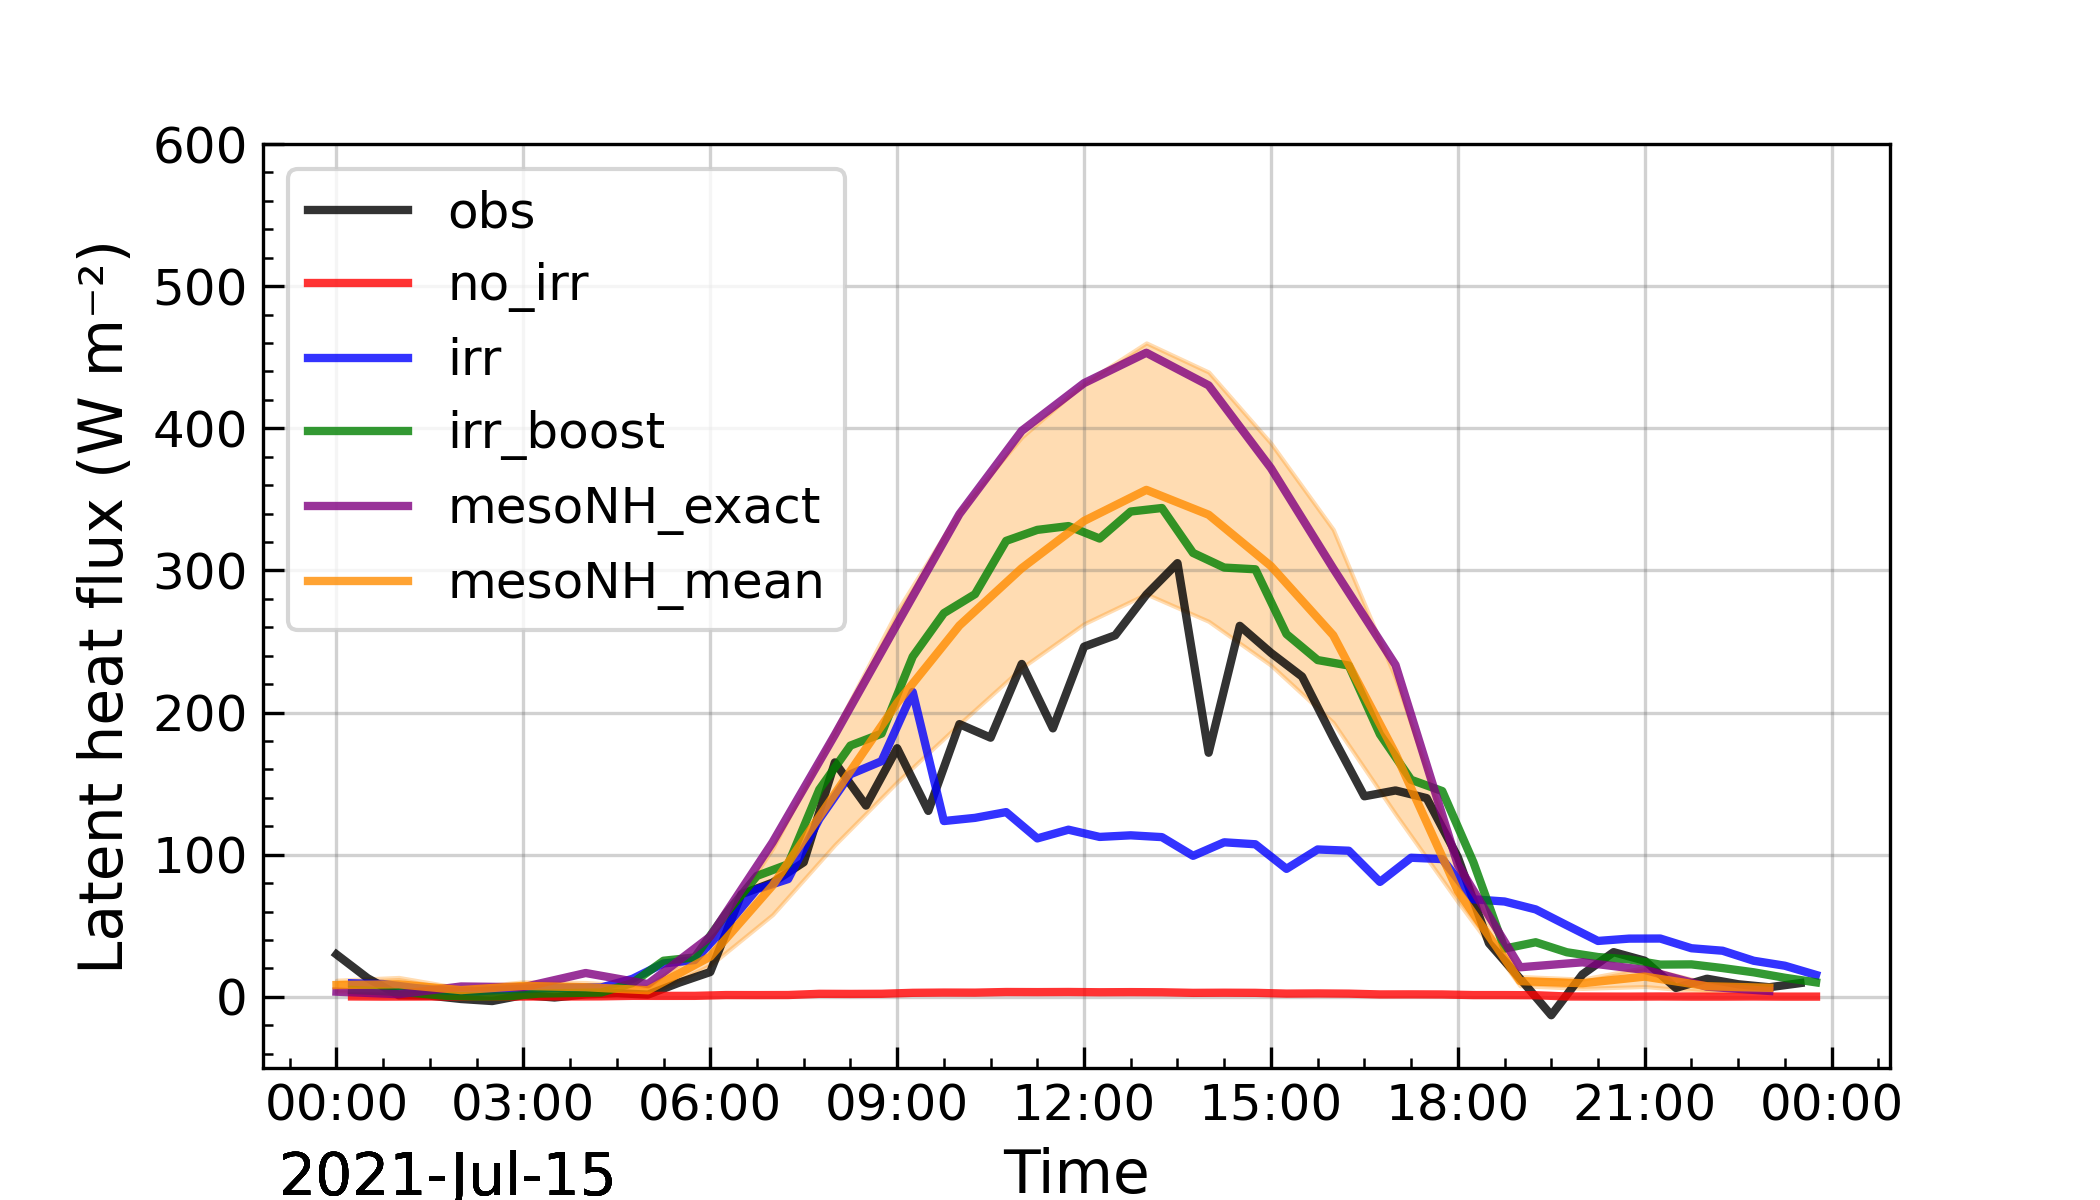
\includegraphics[width=\textwidth]{images/chap6/IOP_TS/TS_2021-07-15_cendrosa_flat.png}
        \end{subfigure} &
        \begin{subfigure}[t]{0.5\textwidth}
            \caption{Latent heat flux\\(20 July - La Cendrosa)}
            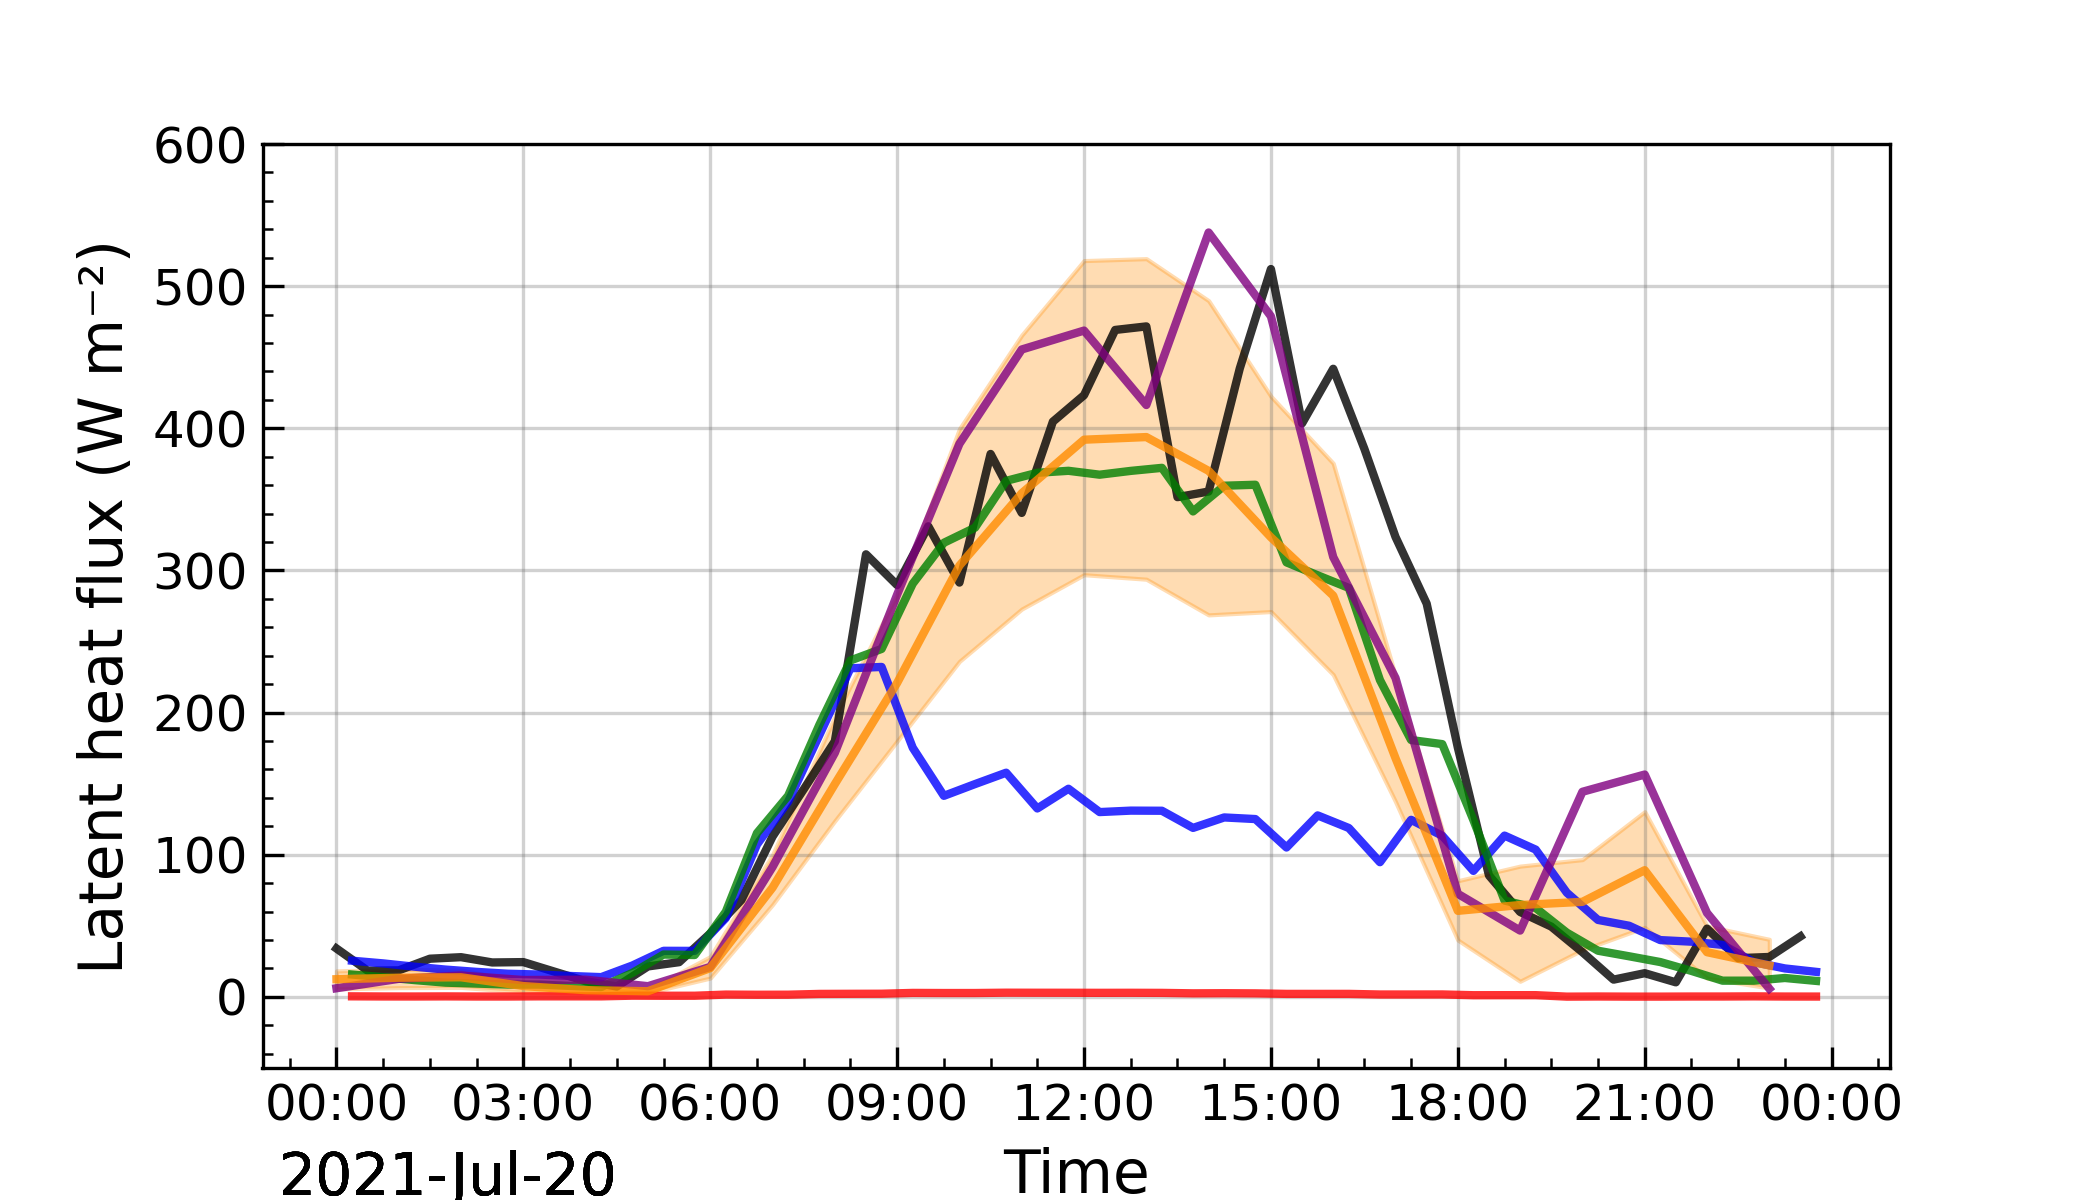
\includegraphics[width=\textwidth]{images/chap6/IOP_TS/TS_2021-07-20_cendrosa_flat.png}
        \end{subfigure} \\
        \begin{subfigure}[t]{0.5\textwidth}
            \caption{Sensible heat flux\\(15 July - La Cendrosa)}
            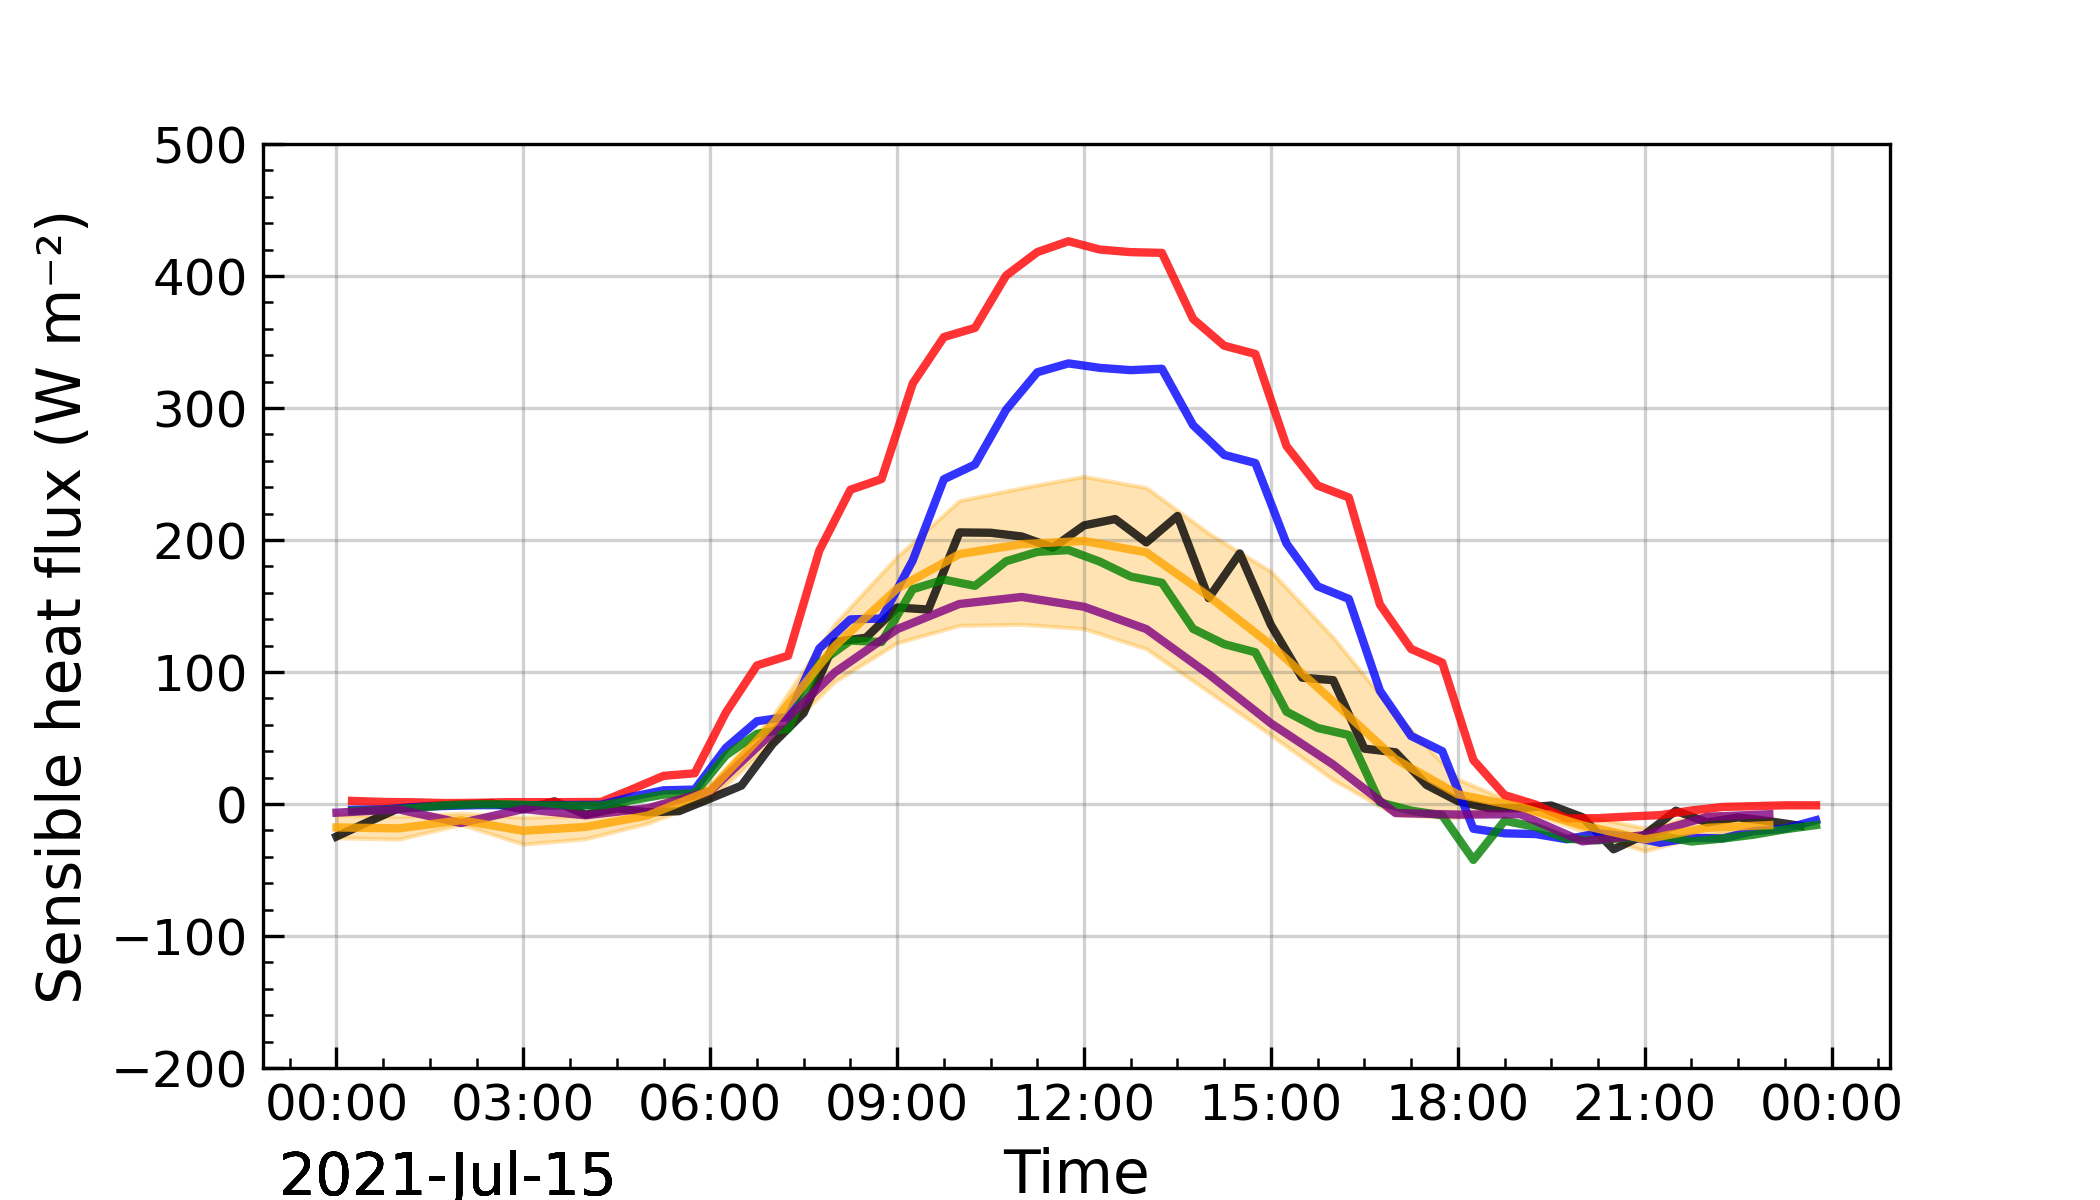
\includegraphics[width=\textwidth]{images/chap6/IOP_TS/TS_2021-07-15_cendrosa_sens.png}
        \end{subfigure} &
        \begin{subfigure}[t]{0.5\textwidth}
            \caption{Sensible heat flux\\(20 July - La Cendrosa)}
            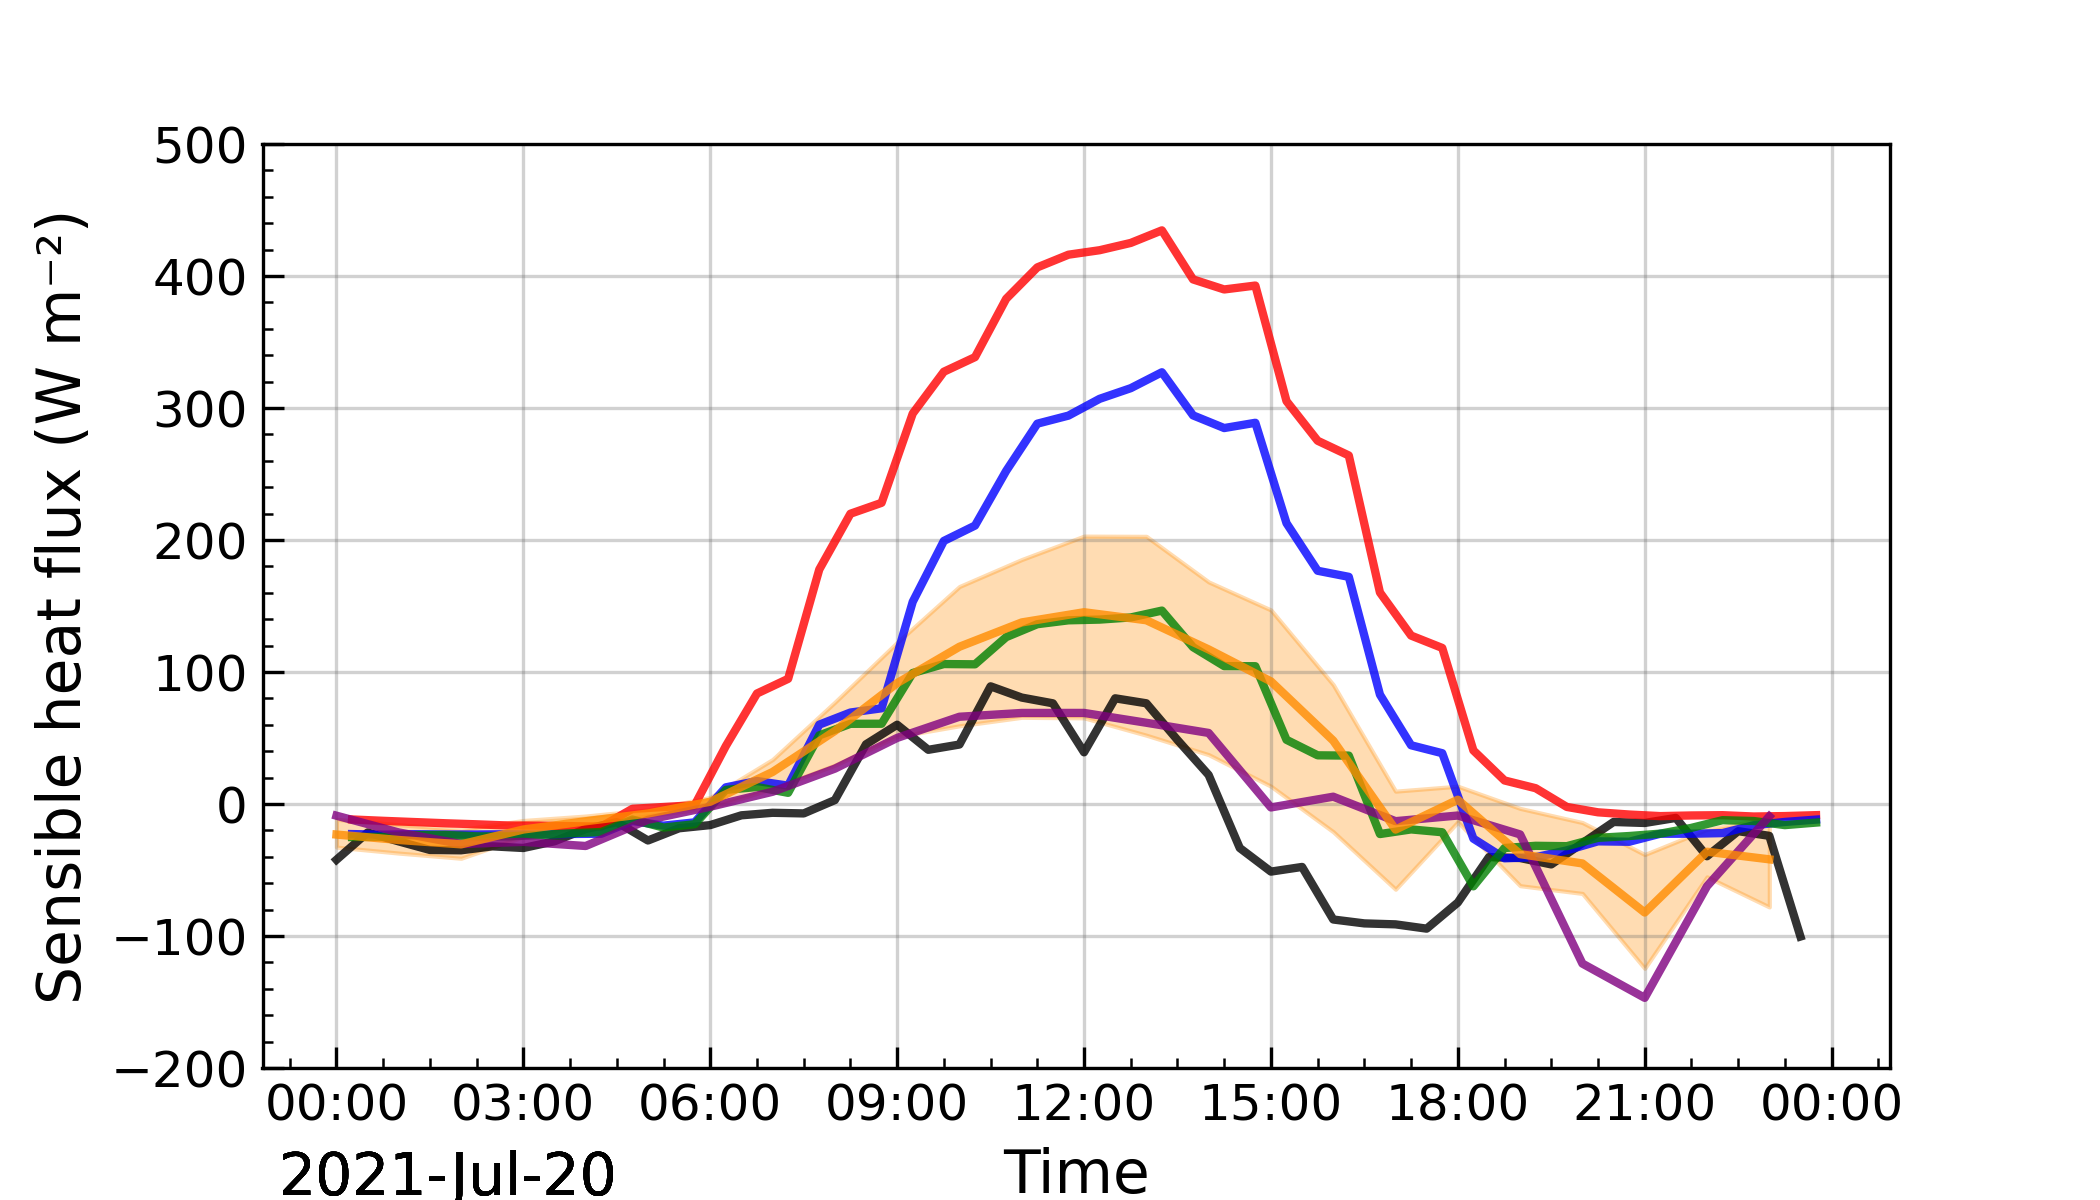
\includegraphics[width=\textwidth]{images/chap6/IOP_TS/TS_2021-07-20_cendrosa_sens.png}
        \end{subfigure} \\
        %rad fluxes
        \begin{subfigure}[t]{0.5\textwidth}
            \caption{Downward shortwave radiation \\(15 July - La Cendrosa)}
            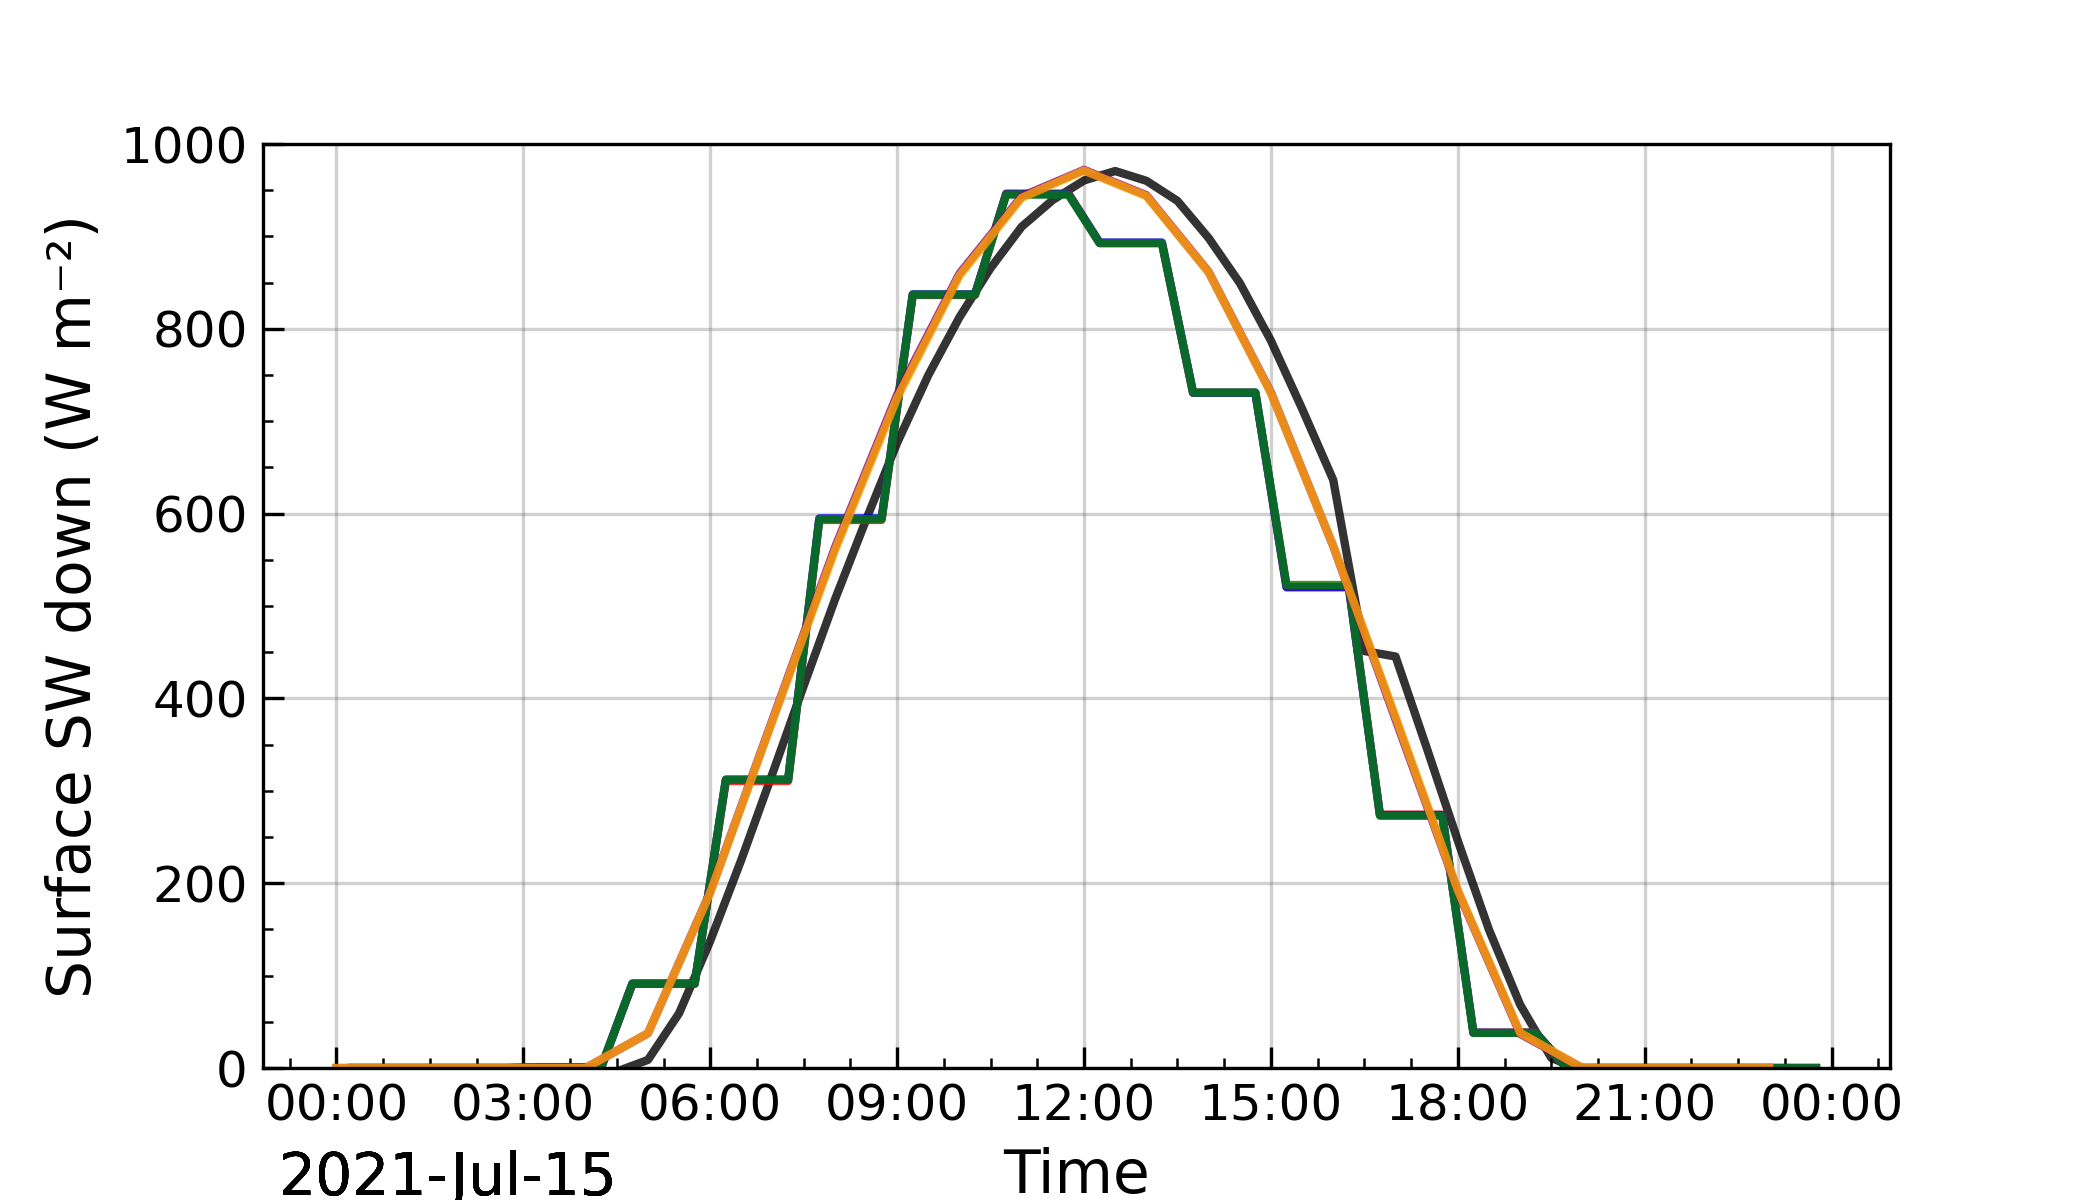
\includegraphics[width=\textwidth]{images/chap6/IOP_TS/TS_2021-07-15_cendrosa_SWdnSFC.png}
        \end{subfigure} &
        \begin{subfigure}[t]{0.5\textwidth}
            \caption{Downward shortwave radiation\\(20 July - La Cendrosa)}
            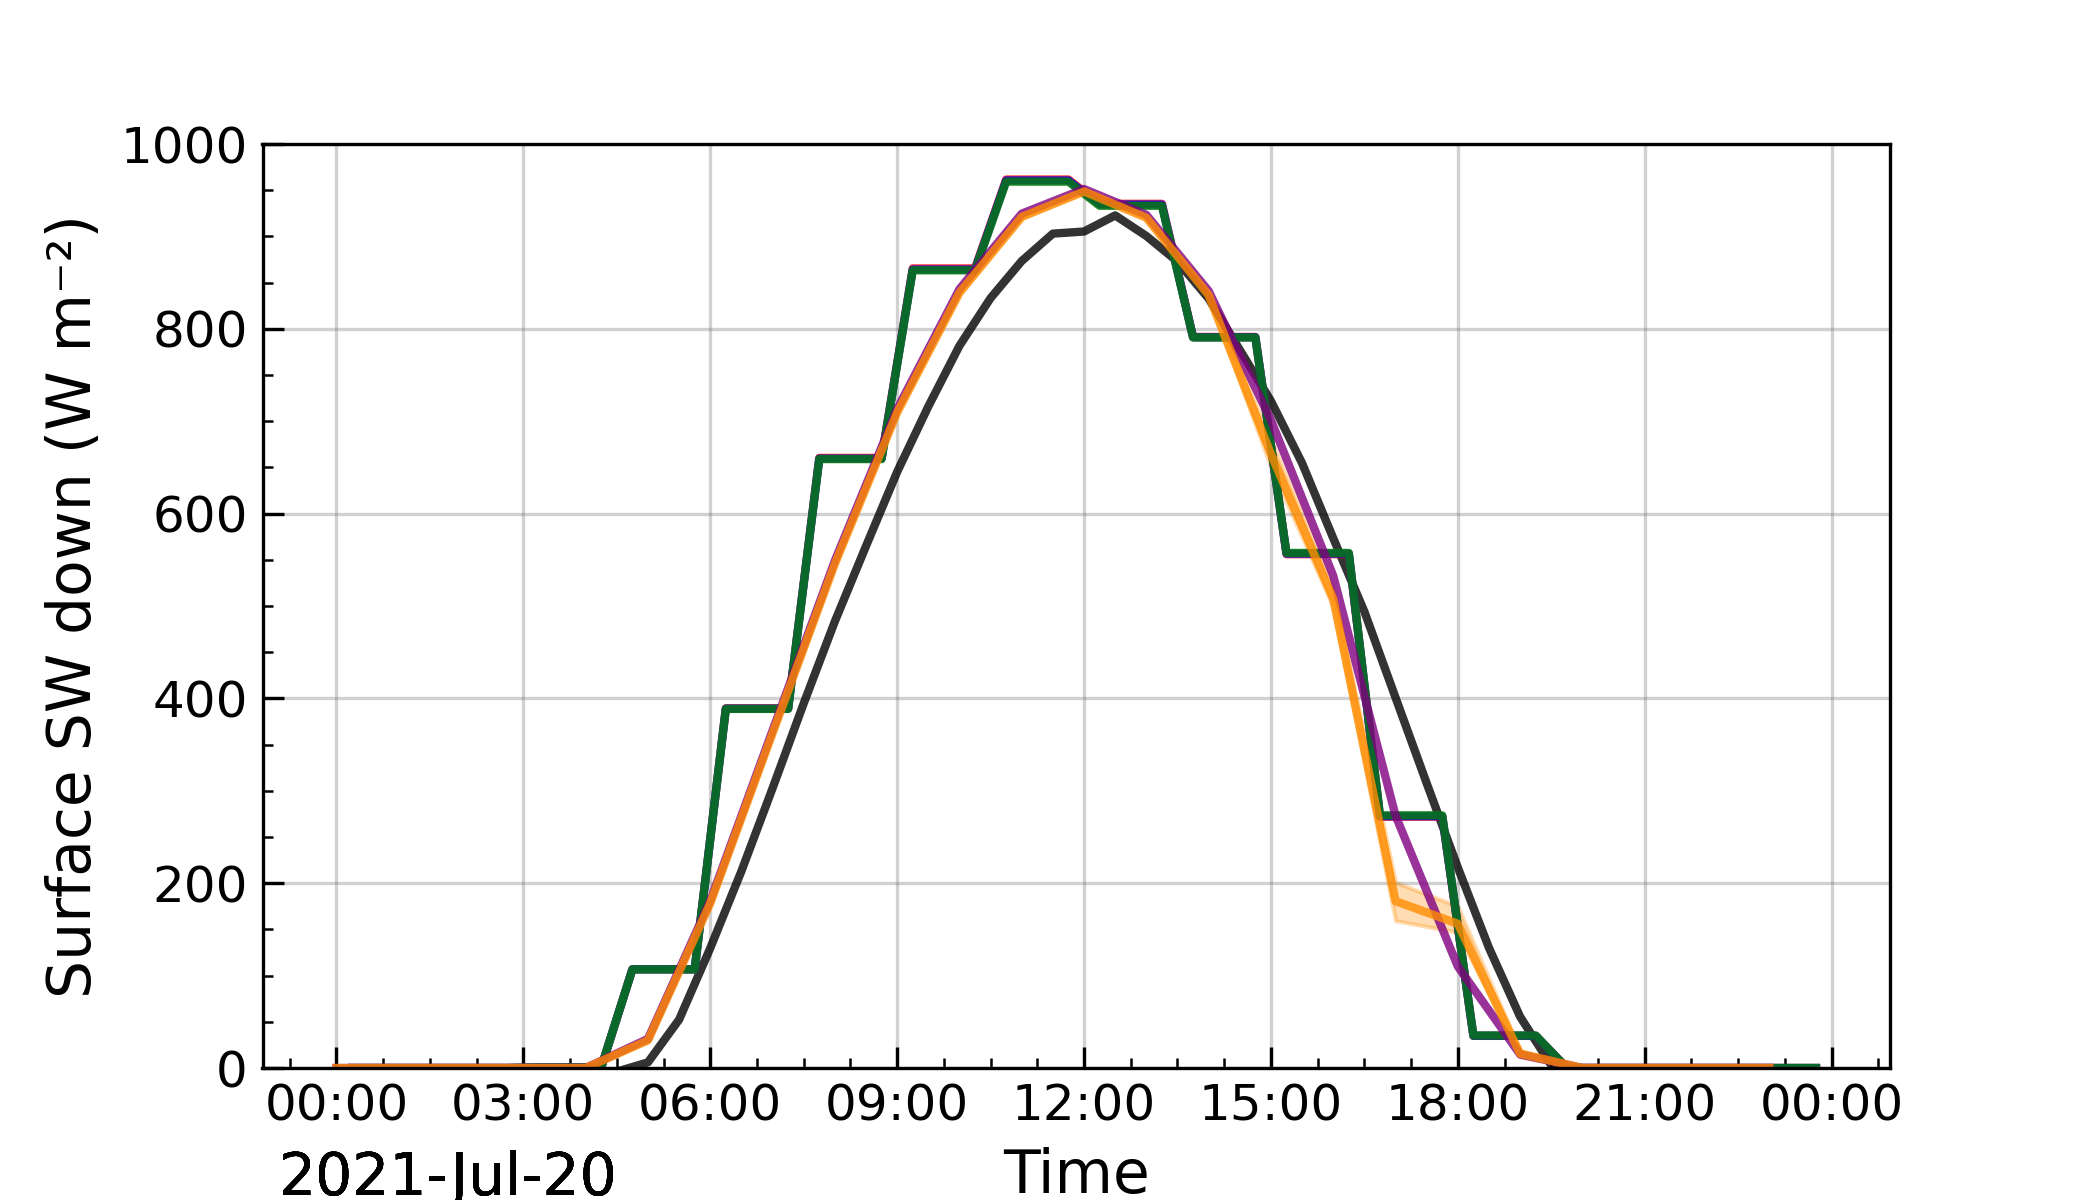
\includegraphics[width=\textwidth]{images/chap6/IOP_TS/TS_2021-07-20_cendrosa_SWdnSFC.png}
        \end{subfigure} \\
        \begin{subfigure}[t]{0.5\textwidth}
            \caption{Downward longwave radiation \\(15 July - La Cendrosa)}
            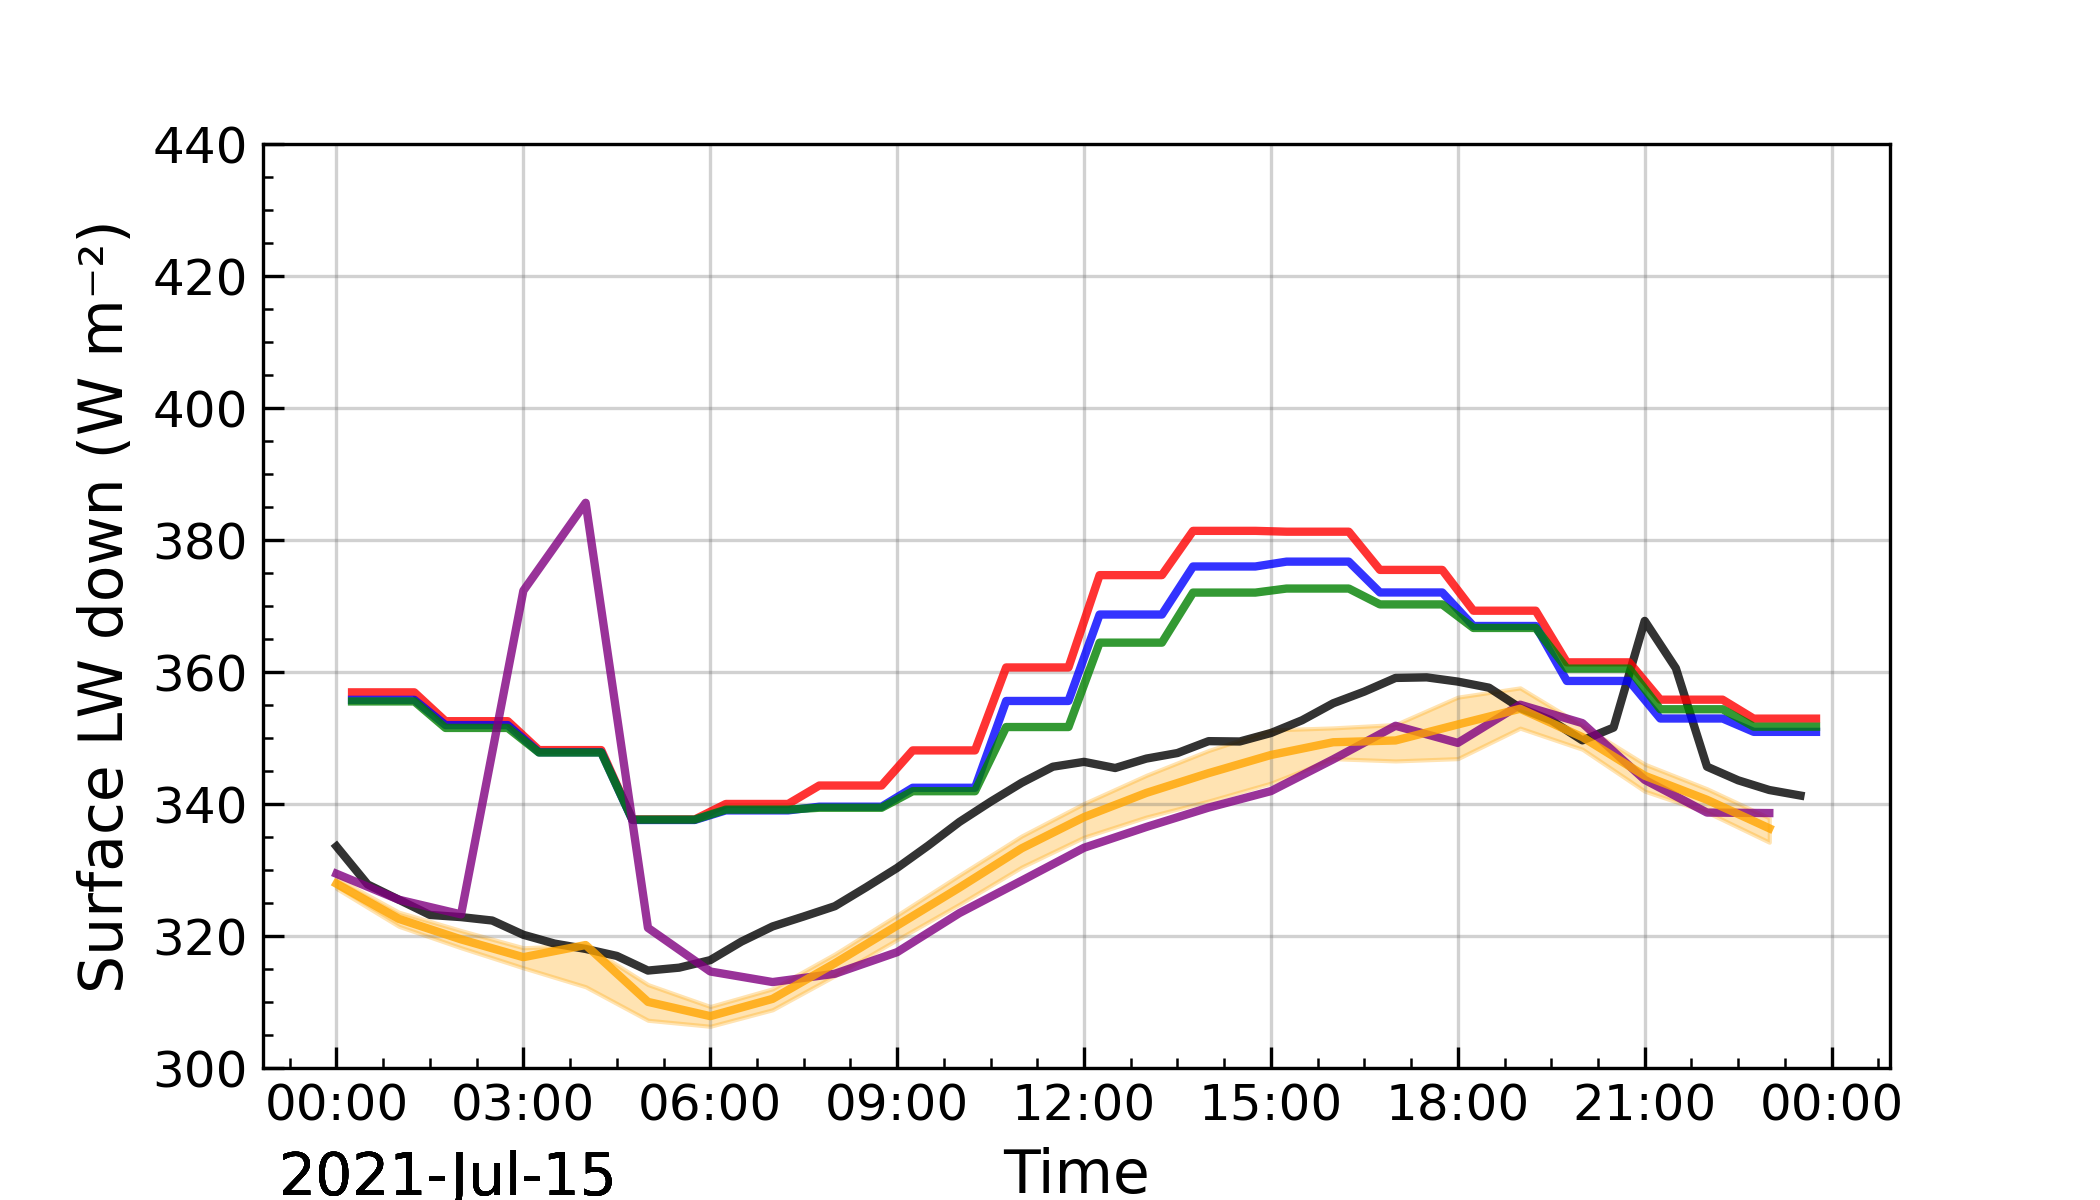
\includegraphics[width=\textwidth]{images/chap6/IOP_TS/TS_2021-07-15_cendrosa_LWdnSFC.png}
        \end{subfigure} &
        \begin{subfigure}[t]{0.5\textwidth}
            \caption{Downward longwave radiation\\(20 July - La Cendrosa)}
            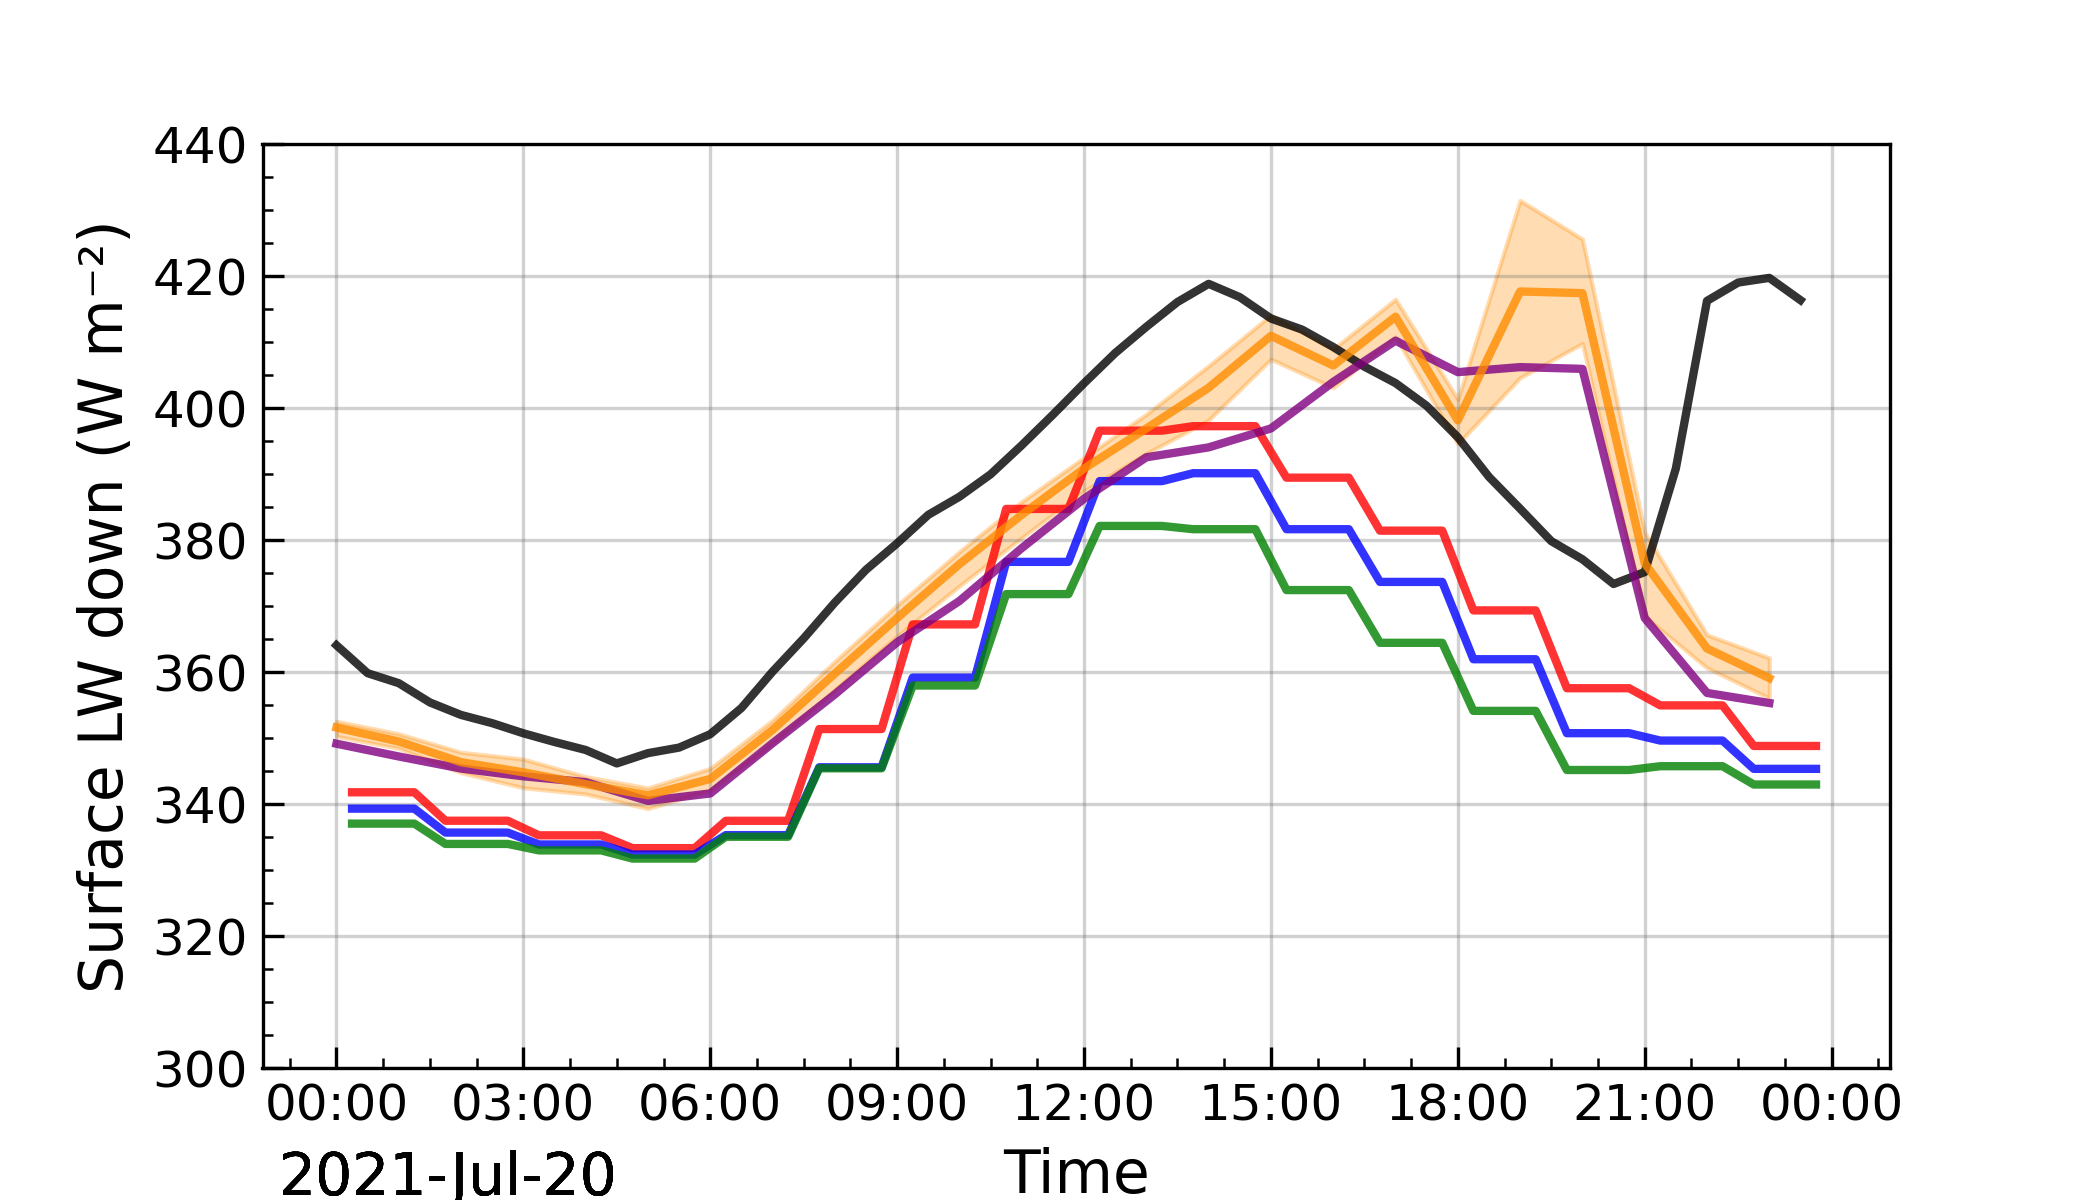
\includegraphics[width=\textwidth]{images/chap6/IOP_TS/TS_2021-07-20_cendrosa_LWdnSFC.png}
        \end{subfigure}
    \end{tabular}
    \caption{Evolution of surface latent (a-b) and sensible (c-d) heat fluxes, downward shortwave (e-f) and longwave (g-h) radiation at La Cendrosa on 15 and 20 July.}
    \label{fig:iop_days_TS_energy}
\end{figure}

\clearpage

\subsection{Impact of irrigation on vertical profiles at 12UTC}
\label{sec:vertical_profiles}

\subsubsection*{15 July 2021}
On 15 July at 12UTC, the surface warm bias seen in ICOLMDZOR seems to be present in all the ABL, where potential temperature is 5K higher than in observations for the \noirr simulation at La Cendrosa (Fig. \ref{fig:profiles_cendrosa_1507}a). 
At Els Plans (Fig. \ref{fig:profiles_cendrosa_1507}e), it is 3-4K higher, which suggests that the bias at La Cendrosa is not only related to irrigation and ET. 
The values of specific humidity in the ABL for the \noirr and \irr simulations are really close to the observations and \mesomean values, indicating that the warm bias is not associated to a dry bias, even in \noirr (Fig. \ref{fig:profiles_cendrosa_1507}b).
Above the ABL, the three ICOLMDZOR simulations converge, and keep exhibiting a warm bias, although smaller than in the ABL, as well as excessive specific humidity, confirming that large-scale advection is imperfectly represented.
At La Cendrosa, the warm bias is reduced by 1K in the \irrboost simulation as surface cooling propagates in the ABL. Specific humidity increases by 1 g \perkg, beyond the observed and \mesomean values, further suggesting that the atmosphere is excessively moist on that day.

%option:mention that above ABL, ICOLMDZOR is too moist ?
On both sites, the ABL height for \noirr and \irr is about 1600 m, which is higher than in observations (800 m at La Cendrosa, 900 at Els Plans). This difference can be attributed to the overestimated surface sensible heat flux in these simulations with little to no irrigation (Fig. \ref{fig:iop_days_TS_energy}c,  \ref{fig:iop_days_TS_energy_elsplans}c). 
In comparison, the ABL is clearly lowered in \irrboost, down to 1200 m, likely through the reduction of the sensible heat flux. This is a good improvement of the structure, but still about 250 m higher than the average ABL height seen in \mesomean, showing that over a grid cell, a good representation of the average surface fluxes does not fully translate into an equally good average ABL structure.
Among the possible causes of such discrepancies in vertical structure are the ABL parametrizations of LMDZ, the influence of subgrid heterogeneities, and variables which are mostly determined by the dynamics. The vertical profiles of wind show that the direction simulated by ICOLMDZOR is mostly correct (Fig. \ref{fig:profiles_cendrosa_1507}d, h), but that wind speed might be too low in most of the ABL on both sites, although is is really similar to \mesomean and \mesoexact (Fig. \ref{fig:profiles_cendrosa_1507}c, g). In theory, an underestimation of wind speed would be associated to a lack of mixing and does not seem to explain the discrepancies. The possible influence of heterogeneities will be discussed in Section \ref{sec:heterogeneities}.
%todo:demander à Etienne et/ou Fred leur avis

\subsubsection*{20 July 2021}

On 20 July at 12UTC, the \noirr simulation presents a warm bias of 2K in potential temperature and a dry bias of 1 to 1.5 g \perkg in the ABL, compared to observations at La Cendrosa (Fig. \ref{fig:profiles_cendrosa_2007}a, b). 
At Els Plans potential temperature is correct in the mixed layer, but there is an even larger dry bias of 2.5 g \perkg (Fig. \ref{fig:profiles_cendrosa_2007}e, f). It must be noted that this is not because ICOLMDZOR simulates a lower specific humidity (in \noirr it is similar on both sites) but rather because the observed values are higher in the rainfed site than in the irrigated site, suggesting a strong impact of non-local processes.
The activation of irrigation at La Cendrosa enables large improvements of the warm and dry biases in \irrboost. Potential temperature is decreased by at least 1K (more than half of the bias), and all the mixed layer benefits from the surface moistening, allowing specific humidity to match the radiosounding profile. 

The ABL height in \noirr is 1200 m at La Cendrosa whereas in the radiosounding, although it remains subject to interpretation, it is more likely around 1400 m, and in Meso-NH it is slightly above 1500 m.
Moreover, there appears to be an internal sublayer up to 500 m, cooler than the rest of the mixed layer, which is also visible in the Meso-NH simulation, where it is also moister. This type of process is unsurprisingly not captured by ICOLMDZOR, which explains why potential temperature in \irrboost matches observations better between 500 m and 900 m.
%option:internal BL ref from Bouzeid (when wind blow perpendicularly its expected) need to remember the proper ref
At Els Plans, the observed profile is easier to interpret with a clear inversion at 1500 m, which is located higher in \mesoexact (around 1650 m) and much lower in ICOLMDZOR simulations (around 850 m).
This cannot be attributed to differences in surface sensible heat flux, since it is higher in ICOLMDZOR simulations than observations (even for \irrboost at La Cendrosa, Fig. \ref{fig:iop_days_TS_energy}d).
Considering that the observed ABL is higher than on 15 July despite a lower surface sensible heat flux (Fig. \ref{fig:iop_days_TS_energy}c-d), the most likely explanation is that ABL development on that day was controlled by other processes, not accounted for in ICOLDMZOR.
In particular, the wind speed at La Cendrosa (Fig. \ref{fig:profiles_cendrosa_2007}c) is two to three times higher in ICOLMDZOR than the observed one in the first 500 m of the atmosphere (and this is the case throughout all morning). %option:link to appendix fig, ajouter mention de la direction (?)
It is similar at Els Plans until 11UTC, but at 12UTC (Fig. \ref{fig:profiles_cendrosa_2007}g), a strong southeasterly wind is observed up to 800 m, and although the direction is rather correct in ICOLMDZOR and Meso-NH, the rapid increase in wind speed is not captured.
In this context, the representation of ABL structure at La Cendrosa is not improved by irrigation since the height of the mixed layer is clearly reduced to 900 m in \irrboost, worsening the limitation identified in \noirr.

\subsubsection*{First conclusions on the impacts of irrigation in the ABL}

The main takeaway from this analysis of vertical profiles is that the impact of irrigation in \irrboost is not limited to surface turbulent fluxes or 2-meter temperature and specific humidity, but also impacts the atmospheric boundary layer.

This allows irrigation to improve the warm bias in the ABL on both days, reducing potential temperature by 1K, and leads to an increase in specific humidity of 1-1.5 g \perkg over La Cendrosa.
These impacts are similar for the two days when considered in absolute value, but their relevance compared to existing biases of ICOLMDZOR depends on the situation.
On 15 July, multiple elements suggest that the 5K bias is not only due to local processes, and it is not very surprising that the impact of irrigation through the surface energy budget is not sufficient to reduce most of the bias in the ABL. On 20 July however, the temperature bias in \noirr is mostly attributable to local processes and a lack of soil moisture at La Cendrosa , which is why it is largely reduced in \irrboost. 
A similar conclusion can be made regarding ABL height. On 15 July, where ABL height was too high in \noirr, irrigation lowers it by 400 m in \irrboost, making it much closer to the \mesomean value. On 20 July, it is lowered by 300 m at La Cendrosa, even though it was already lower than observations and Meso-NH on both sites.

In general, the impact of irrigation on wind speed and direction is quite negligible, except for wind speed around 1000 m above ground level at La Cendrosa on 20 July, where it follows the top of the boundary layer (which is lowered by irrigation).
The impacts on the Els Plans site are also imperceptible, apart from a small moistening of the ABL (0.5 g \perkg at most), visible on both days, which can be explained by advection of moister air from neighbouring irrigated grid cells.

To further investigate the mixing in the ABL and underestand what control its vertical extension on both days, the influence of subgrid heterogeneities was explored in more details.

%Fig : profiles 1507 12UTC
\begin{figure}[hbtp]
    \centering
    \makebox[\textwidth][c]{%
    \begin{tabular}{@{}cccc@{}}
        %cendrosa
        \begin{subfigure}[t]{0.382\textwidth}
            \caption{15 July - La Cendrosa}
            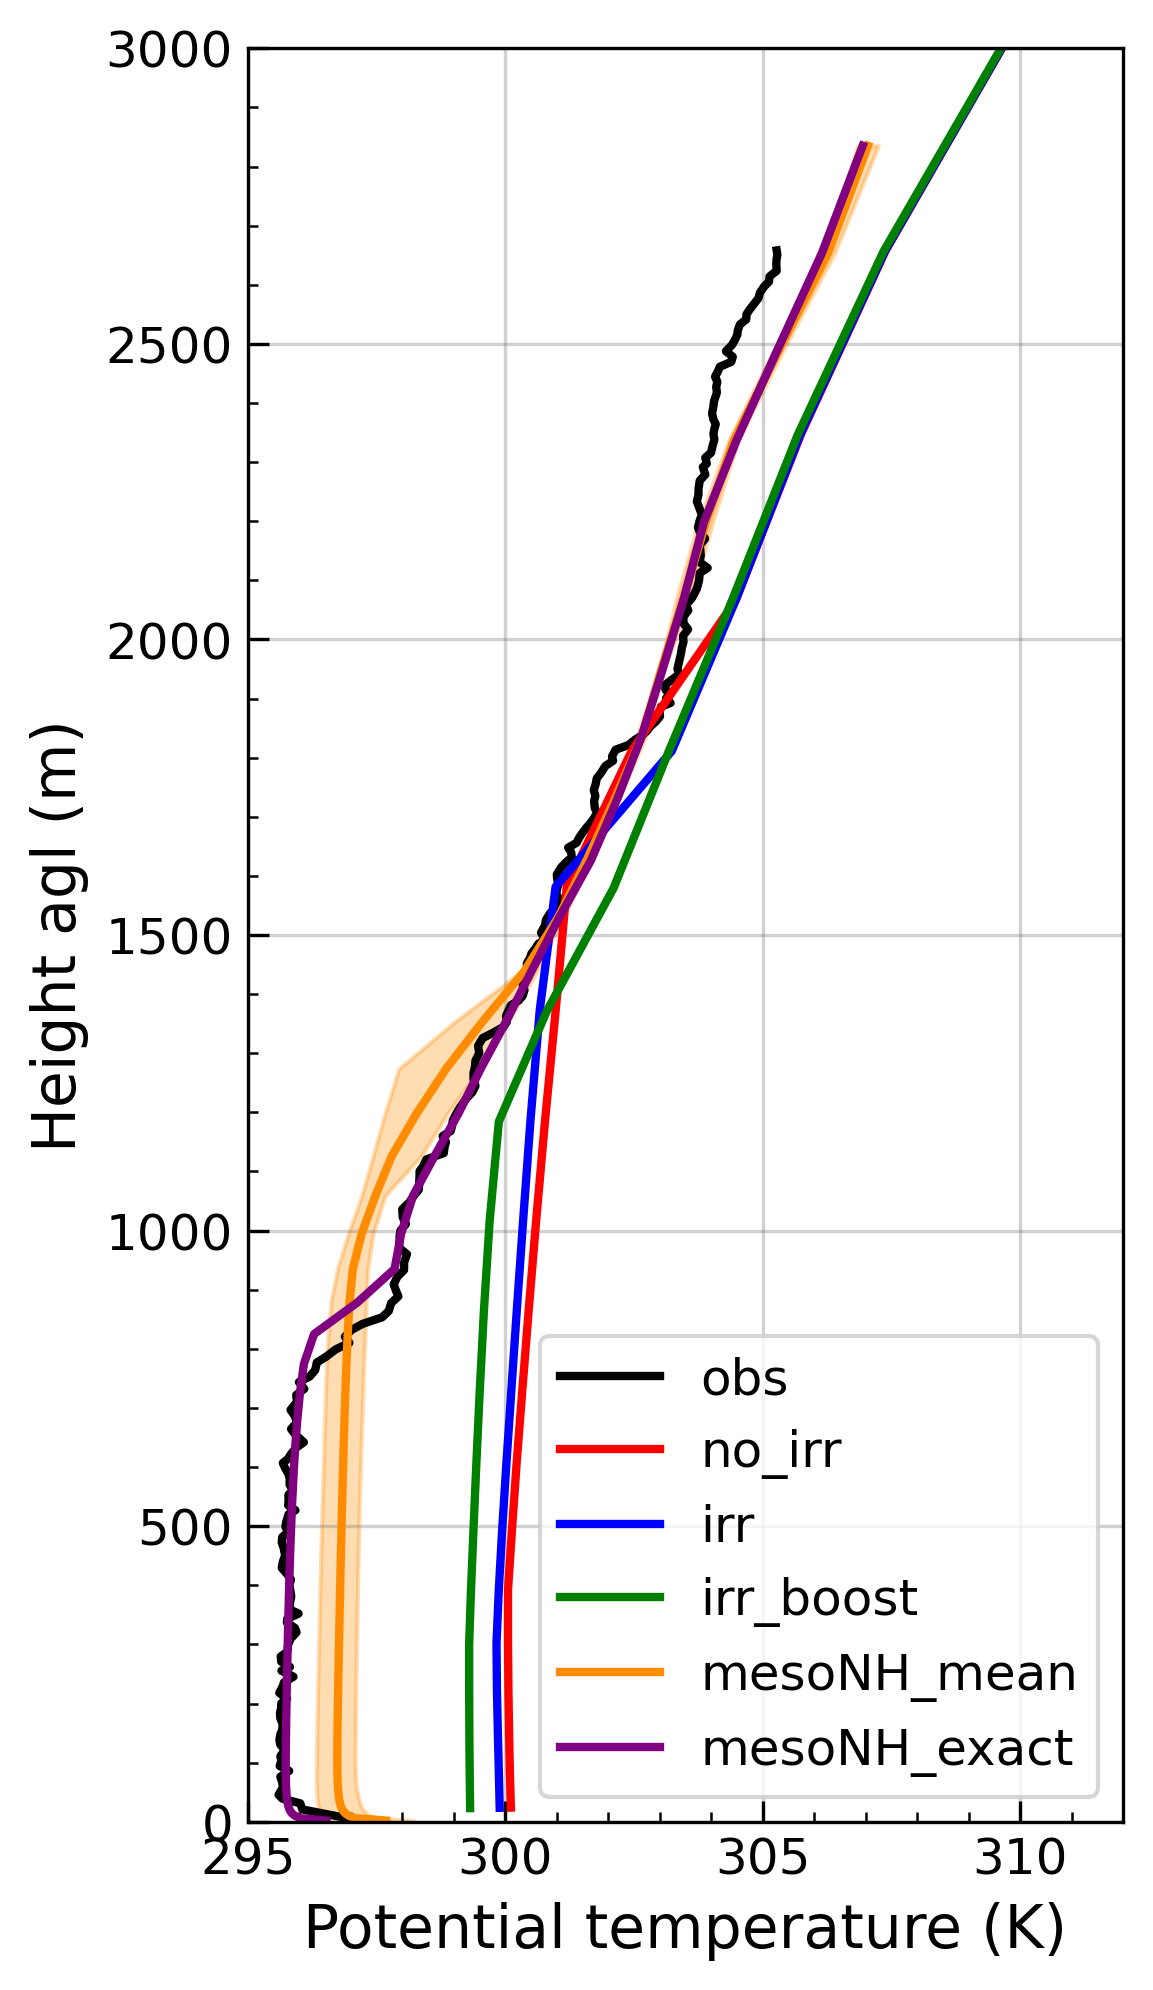
\includegraphics[width=\textwidth]{images/chap6/profiles/profile_cendrosa_theta_1507_.png}
        \end{subfigure} &
        \begin{subfigure}[t]{0.289\textwidth}
            \caption{15 July - La Cendrosa}
            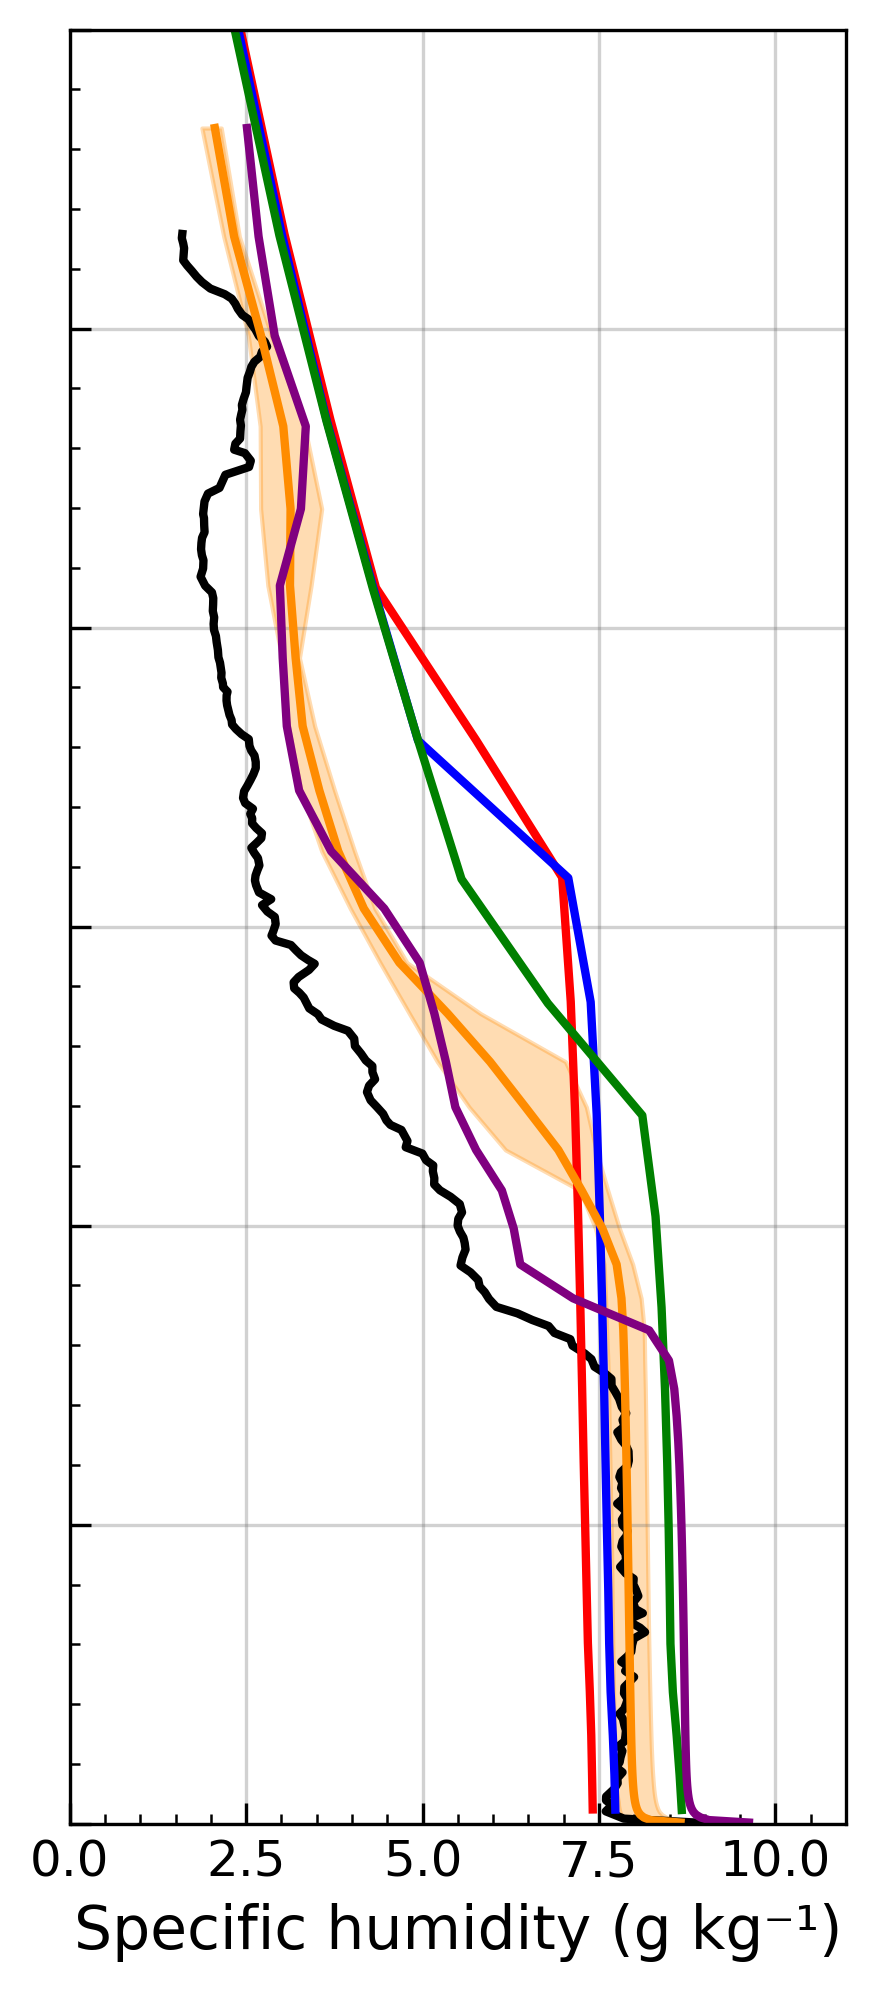
\includegraphics[width=\textwidth]{images/chap6/profiles/profile_cendrosa_ovap_1507_.png}
        \end{subfigure} &
        \begin{subfigure}[t]{0.283\textwidth}
            \caption{15 July - La Cendrosa}
            \includegraphics[width=\textwidth]{images/chap6/profiles/profile_cendrosa_wind_speed_1507_.png}
        \end{subfigure} &
        \begin{subfigure}[t]{0.283\textwidth}
            \caption{15 July - La Cendrosa}
            \includegraphics[width=\textwidth]{images/chap6/profiles/profile_cendrosa_wind_direction_1507_.png}
        \end{subfigure} \\
        %elsplans
        \begin{subfigure}[t]{0.382\textwidth}
            \caption{15 July - Els Plans}
            \includegraphics[width=\textwidth]{images/chap6/profiles/profile_elsplans_theta_1507_.png}
        \end{subfigure} &
        \begin{subfigure}[t]{0.289\textwidth}
            \caption{15 July - Els Plans}
            \includegraphics[width=\textwidth]{images/chap6/profiles/profile_elsplans_ovap_1507_.png}
        \end{subfigure} &
        \begin{subfigure}[t]{0.283\textwidth}
            \caption{15 July - Els Plans}
            \includegraphics[width=\textwidth]{images/chap6/profiles/profile_elsplans_wind_speed_1507_.png}
        \end{subfigure} &
        \begin{subfigure}[t]{0.283\textwidth}
            \caption{15 July - Els Plans}
            \includegraphics[width=\textwidth]{images/chap6/profiles/profile_elsplans_wind_direction_1507_.png}
        \end{subfigure} \\
    \end{tabular}
    }
    \caption{Vertical profiles of observed and simulated potential temperature (a,e), specific humidity (b,f), wind speed (c,g) and direction (d,h) at 12UTC on 15 July, at La Cendrosa (a-d) and Els Plans (e-h).}
    \label{fig:profiles_cendrosa_1507}
\end{figure}

%Fig : profiles 2007 12UTC
\begin{figure}[hbtp]
    \centering
    \makebox[\textwidth][c]{%
    \begin{tabular}{@{}cccc@{}}
        %cendrosa
        \begin{subfigure}[t]{0.382\textwidth}
            \caption{20 July - La Cendrosa}
            \includegraphics[width=\textwidth]{images/chap6/profiles/profile_cendrosa_theta_2007_.png}
        \end{subfigure} &
        \begin{subfigure}[t]{0.289\textwidth}
            \caption{20 July - La Cendrosa}
            \includegraphics[width=\textwidth]{images/chap6/profiles/profile_cendrosa_ovap_2007_.png}
        \end{subfigure} &
        \begin{subfigure}[t]{0.283\textwidth}
            \caption{20 July - La Cendrosa}
            \includegraphics[width=\textwidth]{images/chap6/profiles/profile_cendrosa_wind_speed_2007_.png}
        \end{subfigure} &
        \begin{subfigure}[t]{0.283\textwidth}
            \caption{20 July - La Cendrosa}
            \includegraphics[width=\textwidth]{images/chap6/profiles/profile_cendrosa_wind_direction_2007_.png}
        \end{subfigure} \\
        %elsplans
        \begin{subfigure}[t]{0.382\textwidth}
            \caption{20 July - Els Plans}
            \includegraphics[width=\textwidth]{images/chap6/profiles/profile_elsplans_theta_2007_.png}
        \end{subfigure} &
        \begin{subfigure}[t]{0.289\textwidth}
            \caption{20 July - Els Plans}
            \includegraphics[width=\textwidth]{images/chap6/profiles/profile_elsplans_ovap_2007_.png}
        \end{subfigure} &
        %winds
        \begin{subfigure}[t]{0.283\textwidth}
            \caption{20 July - Els Plans}
            \includegraphics[width=\textwidth]{images/chap6/profiles/profile_elsplans_wind_speed_2007_.png}
        \end{subfigure} &
        \begin{subfigure}[t]{0.283\textwidth}
            \caption{20 July - Els Plans}
            \includegraphics[width=\textwidth]{images/chap6/profiles/profile_elsplans_wind_direction_2007_.png}
        \end{subfigure} \\
    \end{tabular}
    }
    \caption{Vertical profiles of observed and simulated potential temperature (a,e), specific humidity (b,f), wind speed (c,g) and direction (d,h) at 12UTC on 20 July, at La Cendrosa (a-d) and Els Plans (e-h).}
    \label{fig:profiles_cendrosa_2007}
\end{figure}

\clearpage

\subsection{Importance of surface heterogeneities}
\label{sec:heterogeneities}

After noticing the biases in simulated boundary layer height at 12UTC in ICOLMDZOR (overestimation on 15 July and underestimation on 20 July), the influence of surface heterogeneities was investigated, in particular to underestand why representing similar average surface fluxes in \irrboost (compared to \mesomean) is not sufficient to obtain a similar ABL structure.
The objective of this analysis was to determine the dependencies of the \mesomean boundary layer to surface heterogeneities and compare them to the tiled parameter aggregation approach used in ICOLMDZOR, to identify major drivers of ABL development that are misrepresented by not accounting for subgrid heterogeneities. It is a way to assess whether computing one equivalent roughness and one average sensible heat flux for the whole grid cell can realistically propagate the impacts of irrigation in the ABL.

%questions
%does ABL height follow the surface flux heterogeneities in MesoNH ?
%do the driest grid cells in MesoNH have vertical profile similar to noirr, irr ?
%can the limitations of ICOLMDZOR ABL structure be explained by the lack of surface heterogeneity ? When it's too high on 15 July and when it's too low on 20 July ? 

%Fig : bins flux sens
\begin{figure}[hbtp]
    \centering
    \makebox[\textwidth][c]{%
    \begin{tabular}{cc}
        \begin{subfigure}[t]{0.48\textwidth}
            \caption{Sensible heat flux on 15 July at 12UTC}
            \includegraphics[width=\textwidth]{images/chap6/IOP_maps/mesoNH_sens_2021-07-15_12UTC.png}
        \end{subfigure}
        \begin{subfigure}[t]{0.48\textwidth}
            \caption{Sensible heat flux on 20 July at 12UTC}
            \includegraphics[width=\textwidth]{images/chap6/IOP_maps/mesoNH_sens_2021-07-20_12UTC.png} 
        \end{subfigure} \\
        \begin{subfigure}[t]{0.48\textwidth}
            \caption{15 July at 12UTC (La Cendrosa)}
            \includegraphics[width=\textwidth]{images/chap6/IOP_bins/bins_sens_2021-07-15T12:00:00_cendrosa.png}
        \end{subfigure}
        \begin{subfigure}[t]{0.48\textwidth}
            \caption{20 July at 12UTC (La Cendrosa)}
            \includegraphics[width=\textwidth]{images/chap6/IOP_bins/bins_sens_2021-07-20T12:00:00_cendrosa.png}
        \end{subfigure} \\
        \begin{subfigure}[t]{0.48\textwidth}
            \caption{15 July at 12UTC (Els Plans)}
            \includegraphics[width=\textwidth]{images/chap6/IOP_bins/bins_sens_2021-07-15T12:00:00_elsplans.png}
        \end{subfigure}
        \begin{subfigure}[t]{0.48\textwidth}
            \caption{20 July at 12UTC (Els Plans)}
            \includegraphics[width=\textwidth]{images/chap6/IOP_bins/bins_sens_2021-07-20T12:00:00_elsplans.png}
        \end{subfigure}
    \end{tabular}
    }
    \caption{Map of sensible heat flux simulated by Meso-NH at 12UTC on (a) 15 July and (b) 20 July. Corresponding distribution of surface sensible heat flux in \mesomean at La Cendrosa (c-d) and Els Plans (e-f) on both days. Colored crosses indicate the value in the simulations and observations.}
    \label{fig:sens_bins}
\end{figure}

The distribution of sensible heat flux of all the Meso-NH grid cells contributing to \mesomean is represented for the subsets of La Cendrosa and Els Plans on both days at 12UTC, in Fig. \ref{fig:sens_bins}.
It shows that at La Cendrosa (Fig. \ref{fig:sens_bins}a-b), the \mesomean average (orange cross) does not correspond to the majority of Meso-NH grid cells and hides a skewed distribution. This is easily explained since several Meso-NH grid cells fall outside of the irrigated zone, and therefore have a very different surface energy partitioning from the rest.
The ICOLMDZOR \noirr simulation has a sensible heat flux at 12UTC that corresponds to the most extreme values simulated in Meso-NH.
At Els Plans (Fig. \ref{fig:sens_bins}c-d), the distribution is more symetric, although the presence of some irrigated grid cells within the considered ensemble lead to a longer tail of data points with weak sensible heat flux.
On this rainfed site, the three ICOLMDZOR simulations are all very similar and clearly overestimate sensible heat flux on both days, falling outside of the Meso-NH distribution on 15 July, and in the very last bin on July 20.

The excessively high ABL simulated by ICOLMDZOR on 15 July can be attributed to an excessively high sensible heat flux in the \noirr and \irr simulation at La cendrosa, and in all simulations at Els Plans. However, in \irrboost at La Cendrosa, the sensible heat flux matches the average of \mesomean whereas the ABL is still higher. This suggests that the grid-cell mean value of sensible heat flux is not sufficient to describe the ABL structure, and that the ABL height in observations and in Meso-NH is influenced by neighbouring grid cells. In this case, it appears that the mean value of sensible heat flux is being increased by these few grid cells which are not irrigated, but that the ABL height is not impacted in the same way.

\hfill

To look into this, two additional vertical profiles from subsamples at each site are presented alongside the \mesomean profile in Fig. \ref{fig:profiles_theta_ovap_sensbins}. One is the average of grid cells with the lowest values of sensible heat flux at 12UTC (orange dotted line) and the other of the highest values (orange dashed line), respectively encompassing the first and last two bins in Fig. \ref{fig:sens_bins}a-b. 
% 15 July : < 150 and > 400
% 20 July : < 100 and > 375
%option:map of selected grid cells ?

At La Cendrosa on 15 July, it shows that the values of potential temperature and specific humidity are very similar for the two subsamples and the mean value, suggesting that mixing is efficient.
The mean boundary layer is very similar to the low surface sensible heat flux subsample which contains about 50\% of grid cells (Fig. \ref{fig:profiles_theta_ovap_sensbins}a-b). In particular, the inversion is at the same height, suggesting they are the major driver of ABL height in the area. The ABL is higher for the high sensible heat flux subsample, but still much lower than in \noirr and \irr, suggesting that its extent is limited by the neighbouring grid cells, or that the ABL in dry conditions is too high in ICOLMDZOR.

At Els Plans (Fig. \ref{fig:profiles_theta_ovap_sensbins}e-f), there are large differences in potential temperature (more than 2K) and specific humidity (1 g \perkg) between the two subsamples.
ABL structure for the small sensible heat flux subsample is very similar to the one seen at La Cendrosa, and also to the observed profile at Els Plans. For the high sensible heat flux subsample, the ABL is warmer and higher than at La Cendrosa. 
The two subsamples are therefore much more independent of each other at Els Plans than at La Cendrosa, and the observed profile could be interpreted as a combination of two distinct patches with an internal layer influenced by irrigated grid cells and a larger mixed layer corresponding to dry cells (with a second inversion around 1400 m in Fig. \ref{fig:profiles_theta_ovap_sensbins}e-f). 

The difference between the subsets for the two sites might be related to the structure of the heterogeneities, and to the influence of wind direction.
At La Cendrosa, the few non-irrigated grid cells are quite spread out, and surrounded by more irrigated grid cells to the west. At Els Plans, there is a much sharper delineation and the few irrigated grid cells are part of a continuous irrigated patch. 
This can explain why the irrigated grid cells which fall within the Els Plans subset are largely influenced by the other irrigated grid cells to their West. 
The local (south-)westerly low-level winds (Fig. \ref{fig:iop_days_winds}a, c, e, g) increase that influence since they tend to advect the boundary layer of the irrigated patch into the rainfed area, bringing cooler air and moisture.

\hfill

On July 20, the two subsamples are very close to the mean profile for potential temperature and specific humidity on both sites, appart from a cooler and moister 500-meter high sublayer which is only seen for the low sensible heat flux subsamples (Fig. \ref{fig:profiles_theta_ovap_sensbins}c-d). This sublayer, also visble in obserations at La Cendrosa, seems to be the main consequence of heterogeneities in surface fluxes, since the differences on the rest of the ABL structure are rather limited, even at Els Plans.
This type of internal sublayer is not expected to be captured by the LMDZ physics, where mixing is dominated by the EDMF scheme using an average thermal plume \citep{rio_thermal_2008}. 
However, the main limitation of ICOLMDZOR in representing the ABL structure for this day is not related to the presence of this internal boundary layer, but rather the large ABL height underestimation at Els Plans.
On this site, the observed profile is very well mixed with a clear inversion at 1500 m (and 1650 m in \mesoexact), but ICOLMDZOR simulates a 900 m ABL, although it overestimates the surface sensible heat flux.
The most likely driver of ABL development in Meso-NH comes from low-level winds (Fig. \ref{fig:iop_days_winds}b, d, f, h). A strong southeasterly wind  enters the Els Plans area and faces a light northerly wind with a clear front at the border between the irrigated and non-irrigated zones, that extends at least to 950 hPa.
The mixing induced by strong winds and the upward motions associated to the convergence of air are most likely the cause for the very high ABL on 20 July (higher than on 15 July despite lower sensible heat fluxes in both observations and Meso-NH). 
%option:mention that this front is present in previous hours as well ?
Above the front, higher altitude southeasterly winds seem to partly advect that well developed mixed layer into the irrigated zone, above the internal boundary layer, contributing to the more complex vertical profiles at La Cendrosa.
Some further investigation could help determine if the location of the front is mainly dictated by the difference in roughness or by pressure gradients between the two zones, but it seems clear that subgrid heterogeneities is surface sensible heat flux is not a first order driver of ABL development.
This explains why the irrigation parametrization could not improve the ABL structure over the area in the current state of the model, which does not account for the impact of the observed front on the ABL.

% Fig : profiles with sens bins min/max theta and ovap
\begin{figure}[hbtp]
    \centering
    \makebox[\textwidth][c]{%
    \begin{tabular}{@{}cccc@{}}
        %cendrosa
        %1507
        \begin{subfigure}[t]{0.382\textwidth}
            \caption{15 July - La Cendrosa}
            \includegraphics[width=\textwidth]{images/chap6/profiles/profile_cendrosa_theta_1507_sensbins.png}
        \end{subfigure} &
        \begin{subfigure}[t]{0.29\textwidth}
            \caption{15 July - La Cendrosa}
            \includegraphics[width=\textwidth]{images/chap6/profiles/profile_cendrosa_ovap_1507_sensbins.png}
        \end{subfigure} &
        %2007
        \begin{subfigure}[t]{0.285\textwidth}
            \caption{20 July - La Cendrosa}
            \includegraphics[width=\textwidth]{images/chap6/profiles/profile_cendrosa_theta_2007_sensbins.png}
        \end{subfigure} &
        \begin{subfigure}[t]{0.29\textwidth}
            \caption{20 July - La Cendrosa}
            \includegraphics[width=\textwidth]{images/chap6/profiles/profile_cendrosa_ovap_2007_sensbins.png}
        \end{subfigure} \\
        %elsplans
        %1507
        \begin{subfigure}[t]{0.382\textwidth}
            \caption{15 July - Els Plans}
            \includegraphics[width=\textwidth]{images/chap6/profiles/profile_elsplans_theta_1507_sensbins.png}
        \end{subfigure} &
        \begin{subfigure}[t]{0.29\textwidth}
            \caption{15 July - Els Plans}
            \includegraphics[width=\textwidth]{images/chap6/profiles/profile_elsplans_ovap_1507_sensbins.png}
        \end{subfigure} &
        %2007        
        \begin{subfigure}[t]{0.285\textwidth}
            \caption{20 July - Els Plans}
            \includegraphics[width=\textwidth]{images/chap6/profiles/profile_elsplans_theta_2007_sensbins.png}
        \end{subfigure} &
        \begin{subfigure}[t]{0.29\textwidth}
            \caption{20 July - Els Plans}
            \includegraphics[width=\textwidth]{images/chap6/profiles/profile_elsplans_ovap_2007_sensbins.png}
        \end{subfigure} \\
    \end{tabular}
    }
    \caption{Vertical profiles of potential temperature and specific humidity at 12UTC at La Cendrosa (a-d) and Els Plans (e-h), on 15 July and 20 July. Additional orange lines show the mean profile for the minimum (dotted) and maximum (dashed) sensible heat fux subsamples (first and last two bins on Fig. \ref{fig:sens_bins}).}
    \label{fig:profiles_theta_ovap_sensbins}
\end{figure}

%Fig : MesoNH winds Cendrosa
\begin{figure}[hbtp]
    \centering
    \begin{tabular}{cc}
        %10m
        \begin{subfigure}[t]{0.5\textwidth}
            \caption{15 July at 10 m}
            \includegraphics[width=\textwidth]{images/chap6/IOP_maps/mesoNH_wind_10m_2021-07-15T12:00:00.png}
        \end{subfigure} &
        \begin{subfigure}[t]{0.5\textwidth}
            \caption{20 July at 10 m}
            \includegraphics[width=\textwidth]{images/chap6/IOP_maps/mesoNH_wind_10m_2021-07-20T12:00:00.png}
        \end{subfigure} \\
        %950hPa
        \begin{subfigure}[t]{0.5\textwidth}
            \caption{15 July at 950 hPa}
            \includegraphics[width=\textwidth]{images/chap6/IOP_maps/mesoNH_wind_950_2021-07-15T12:00:00.png}
        \end{subfigure} &
        \begin{subfigure}[t]{0.5\textwidth}
            \caption{20 July at 950 hPa}
            \includegraphics[width=\textwidth]{images/chap6/IOP_maps/mesoNH_wind_950_2021-07-20T12:00:00.png}
        \end{subfigure} \\
        %900hPa
        \begin{subfigure}[t]{0.5\textwidth}
            \caption{15 July at 900 hPa}
            \includegraphics[width=\textwidth]{images/chap6/IOP_maps/mesoNH_wind_900_2021-07-15T12:00:00.png}
        \end{subfigure} &
        \begin{subfigure}[t]{0.5\textwidth}
            \caption{20 July at 900 hPa}
            \includegraphics[width=\textwidth]{images/chap6/IOP_maps/mesoNH_wind_900_2021-07-20T12:00:00.png}
        \end{subfigure} \\
        %850hPa
        \begin{subfigure}[t]{0.5\textwidth}
            \caption{15 July at 850 hPa}
            \includegraphics[width=\textwidth]{images/chap6/IOP_maps/mesoNH_wind_850_2021-07-15T12:00:00.png}
        \end{subfigure} &
        \begin{subfigure}[t]{0.5\textwidth}
            \caption{20 July at 850 hPa}
            \includegraphics[width=\textwidth]{images/chap6/IOP_maps/mesoNH_wind_850_2021-07-20T12:00:00.png}
        \end{subfigure} \\
    \end{tabular}
    \caption{Wind speed simulated by Meso-NH over the LIAISE observations sites at 12UTC on 15 and 20 July, at 10m (a-b), 950hPa (c-d), 900hPa (e-f), and 850hPa (g-h).}
    \label{fig:iop_days_winds}
\end{figure}

\clearpage

\section{Chapter conclusions}

This chapter used the simulation setup used in Chapters \ref{chap:monthly} to compare the ICOLMDZOR LAM to local observations from the LIAISE campaign and Meso-NH simulations at 2-kilometer resolution.
Two grid cells were selected for the LIAISE observation sites of La Cendrosa (irrigated alfalfa crops) and Els Plans (rainfed low vegetation), in the eastern Ebro basin.
The basic comparison of the \noirr and \irr simulations quickly identified a shortage of water that did not allow the irrigation scheme to sustain irrigation demand. This was already identified generally in Chapter \ref{chap:monthly} mostly for southern regions of the Iberian Peninsula, but also applied to the study area and period of the LIAISE campaign. It can partly be explained because actual irrigation relies on water adduction from the Pyrenees by the Canal d'Urgell, which is not represented in the model.
Due to this lack of water, the \irr simulation shows little differences with \noirr, since latent heat flux could only be partially increased during the day and did not follow the structure of the observed diurnal cycle.

The \irrboost simulation was therefore conducted as a sensitivity experiment, lifting the limits on available water for the month of July 2021.
At La Cendrosa, this enabled simulated irrigation to match irrigation demand, and latent heat flux to follow a complete diurnal cycle. On average over the LIAISE SOP \irrboost largely reduced the biases to observed values of turbulent fluxes, 2-meter temperature and humidity and slightly reduced the excessive wind speed. 
One limitation of these improvements not analyzed here, is that this increase in evapotranspiration in ORCHIDEE was mostly ($\sim$75\%) driven by bare soil evaporation rather than plant transpiration, which is not considered realistic, but has been identified in other LSM \citep{marti_implementation_2025}. %option: figure en Appendix ? 
This might be attributed to an insufficient development of vegetation, but also to the partitioning of ET between its components, which could be another direction to explore to improve surface-atmosphere interactions in irrigated areas.
%option:soil moisture data here....
Surface variables at Els Plans, however, as well as wind directions, were not affected by simulated irrigation, showing almost no non-local effects of irrigation, appart from a small moistening in the day.
This lack of dynamical response to irrigation was expected considering that the lifting of water supply limitations in \irrboost only applied to a few grid cells, including some areas that do not actually receive large irrigation. This setup was mostly designed for an exploration of local processes which seemed a reasonable objective considering the 25-kilometer resolution of ICOLMDZOR relative to the size of the main irrigated patch in the LIAISE study area (about 20 km). The Els Plans site was therefore mostly used to isolate the biases of the model that cannot be attributed to irrigation and help analyzing the situation at La Cendrosa.

In addition to the observations, ICOLMDZOR was also compared to the Meso-NH simulations, particularly by aggregating all the Meso-NH grid cells of each ICOLMDZOR grid cell into one average value (\mesomean). At La Cendrosa, this showed that even when the \irrboost simulation is not matching the observed values, it is very close \mesomean, especially for turbulent fluxes, but also on temperature and humidity during the day. 
The demonstrates that the tiled approach for irrigation and the parameter aggregation framework enables ORCHIDEE to properly represent average surface fluxes over the grid cell.

\hfill

The question of whether this good performance on surface variables was also observed in the boundary layer was investigated using vertical profiles of the atmosphere. Out of the seven IOP days on which radiosoundings were conducted on both sites, two were selected (15 and 20 July), each representative of a part of the SOP with different characteristics.

Vertical profiles confirmed that the effects of simulation irrigation in ICOLMDZOR extend into the entire ABL, with systematic cooling and moistening at La Cendrosa. There was no noticeble impact on winds, and at Els Plans, a small moistening was also visible, meaning that a portion of the additional atmospheric moisture provided by irrigation can be advected to a non-irrigated grid cell.
The two IOP days showed different limitations of ICOLMDZOR regarding the boundary layer: on 15 July specific humidity was correct but potential temperature was too high, whereas on 20 July, temperature was closer to expected values, but a dry bias was observed, and the ABL was much lower than observations and Meso-NH.
At La Cendrosa, \irrboost irrigation was only able to reduce a small part of the warm bias on 15 July, but led to an overestimated specific humidity, whereas on 20 July, it allowed the potential temperature and specific humidity to match observations much better, showing that its impact is much more relevant when biases are linked to local processes.

Regarding boundary layer structure however, it is mostly on 15 July that the impact of irrigation was positive, since it lowered the excessively high ABL. It was still not perfectly matching the observed profile however, and still presented a higher ABL than the \mesomean value. 
On 20 July, irrigation also contributed to a lower boundary layer but did not enable a better match with the expected profile. 
To better understand the limitations identified in these two IOP days, surface heterogeneities of fluxes were explored in more detail.

\hfill

Considering the choice of having no irrigation at all at Els Plans, this analysis of heterogeneity focused mostly on La Cendrosa, but, as for surface variables the Els Plans grid cell still served as a reference to understand the behaviour of the model and the ABL structure over the area.
It was shown that the \mesomean average value at La Cendrosa was due to a very skewed distribution with a large majority of irrigated grid cells. 
On 15 July, the subsample of non-irrigated grid cells seems to have a large impact on the mean sensible heat flux, but not to be major drivers of the mean ABL development. ICOLMDZOR does not account for this aspect in taking only the an average sensible heat flux, and this can partly explain why it is still simulating an excessively high ABL even with the appropriate surface fluxes.

On 20 July, the development of the ABL simulated by Meso-NH at Els Plans seems partly driven by a front of intense southeasterly wind that follows the delineation between the irrigated and non-irrigated area, which likely contributes to an intense mixing and elevation of the ABL to 1500 m. 
This also seems to explain the complex structure of the ABL seen at La Cendrosa, with a very high ABL that is partly advected from the rainfed area, and a cooler and moister sublayer over the irrigated grid cells. 
The LMDZ physics are not designed to represent such ABL sub-structures which depend more on heterogeneities of wind of surface fluxes, and can therefore not be greatly improved by irrigation.

More generally, the analysis of the two selected days confirmed that the influence of surface heterogeneities is strongly dependent their structure and on the local wind regime. 
In particular, the direction of the wind relative to the borders between patches of different surface conditions drives the influence of these patches on one another.
When the low-level wind is perpendicular to the border (as seen at Els Plans on both days or La Cendrosa on 20 July), the ABL is generally well mixed but can lead to the presence of internal sublayers \citep[as reviewed in][]{bou-zeid_persistent_2020}. When the wind is parallel to the border, different ABL structures coexist side by side and their development is largely conditioned by surface fluxes (as seen at Els Plans on 15 July on Fig. \ref{fig:profiles_theta_ovap_sensbins}e-f).
Out of the four situations examined here (2 grid cells on 2 distinct days), the assumptions associated to the use of a single atmospheric column for the grid cell seem to hold, but this is not the case when the wind is aligned with the border between irrigated and non-irrigated land.

\clearpage

